\setcounter{excounter}{1}
\setcounter{examplecounter}{1}
\chapter{Arrays, Collections, and Generics}
\label{chapter-arrays-collections} % Always give a unique label
% use \chaptermark{}
% to alter or adjust the chapter heading in the running head

\abstract*{Each chapter should be preceded by an abstract (no more than 200 words) that summarizes the content. The abstract will appear \textit{online} at \url{www.SpringerLink.com} and be available with unrestricted access. This allows unregistered users to read the abstract as a teaser for the complete chapter.
Please use the 'starred' version of the new \texttt{abstract} command for typesetting the text of the online abstracts (cf. source file of this chapter template \texttt{abstract}) and include them with the source files of your manuscript. Use the plain \texttt{abstract} command if the abstract is also to appear in the printed version of the book.}

\abstract{Each chapter should be preceded by an abstract (no more than 200 words) that summarizes the content. The abstract will appear \textit{online} at \url{www.SpringerLink.com} and be available with unrestricted access. This allows unregistered users to read the abstract as a teaser for the complete chapter. \newline\indent
Please use the 'starred' version of the new \texttt{abstract} command for typesetting the text of the online abstracts (cf. source file of this chapter template \texttt{abstract}) and include them with the source files of your manuscript. Use the plain \texttt{abstract} command if the abstract is also to appear in the printed version of the book.}

\section{Arrays}

Thus far, all data that we work with has been passed as method parameters. 
When we invoke a method, we have access to the arguments at that point in time. 
\emph{Arrays} allow us to store values, similar to how we use variables, but with the added benefit of storing multiple values in one location.

Arrays store \emph{elements} and \emph{indices} of some type. 
An element is just a value in an array. 
The \emph{index} of an element is its location in the array. 
Indices of an array are indexed from zero, much like strings. 
Thus, the first element of an array is at index zero, whereas the last element is located at the index $|A| - 1$, where $|A|$ denotes the number of elements, or \emph{cardinality}, of some array~$A$.

We store elements contiguously in arrays, where all are of the same type. 
This means that, if we declare an array of type \ttt{int}, we cannot store, for example, a \ttt{String} in that array. 
We can declare an array variable with preset values using \emph{initializer lists}\index{initializer lists}:

\begin{verbnobox}[\small]
int[] array = {5, 10, 15, 20, 100, 50};
\end{verbnobox}

To retrieve the size of an array, the number of elements it can store, we access the \emph{.length} field of the array, e.g., \ttt{array.length}. 
For our example array, we see that its size is six. 
Moreover, \ttt{array[0]} stores \ttt{5}, and \ttt{array[5]} stores \ttt{50}. 
Accessing a negative index or an index beyond the bounds of the length results in an \ttt{ArrayIndexOutOfBoundsException}. 
So, accessing \ttt{array[-1]} or \ttt{array[6]}, for instance, crashes the program. 
A common mistake is to access the index at the length of the array to retrieve the last element, which represents a misunderstanding of array indexing.

To declare an array of type~$T$, called~$A$, that stores~$N$ elements, we write the following:

\begin{verbnobox}[\small]
T[] A = new T[N];
\end{verbnobox}

We can store a value~$e$ at an arbitrary index~$i$ of array~$A$, in addition to accessing the value at some index.

\begin{verbnobox}[\small]
// Store "e" at index i of A.
A[i] = e;
// Print out the value at A[i].
System.out.println(A[i]);
\end{verbnobox}

\myexample{Let's declare an integer array~$A$ to store the integers from zero to one hundred in increments of ten.}
\begin{verbnobox}[\small]
int[] A = {0, 10, 20, 30, 40, 50, 60, 70, 80, 90, 100};
\end{verbnobox}

Initializer lists are verbose and require us to explicitly specify each individual constant. 
A better solution is to initialize the array to a size, and populate its elements using a loop.

\begin{verbnobox}[\small]
final int SIZE = 11;
int[] A = new int[SIZE];
for (int i = 0; i < A.length; i++) { A[i] = i * 10; }
\end{verbnobox}

We use~$i$ to iterate over the possible indices of our array. 
Before we explained that~$i$ is used out of standard loop convention, but we now say that~$i$, in general, stands for either ``iteration'' or ``index.'' 
We assign, to~$A$ at index $i$, the value of $i$ multiplied by ten. 
We can convert the array to a \ttt{String} using a utility method from the \ttt{Arrays} class (note the plural!); a ``string-ified'' array separates each element by commas and surrounds them with braces.

\begin{verbnobox}[\small]
String s1 = Arrays.toString(A);
s1 => {0, 10, 20, 30, 40, 50, 60, 70, 80, 90, 100}
\end{verbnobox}

\begin{figure}[tp]
%\begin{wrapfigure}[25]{r}[0.75in]{0.55\textwidth}
  \small
  \begin{tcolorbox}[title=Java Arrays]
    An \emph{array}\index{array} stores a fixed-size collection of elements of some type.
    \vspace{2ex}
    % \hrule
    % \vspace{2ex}
  \begin{description}
    \item [\ttt{$T[]\;A =$ new $T[n]$}] creates an array of type $T$, named $A$, that stores $n$ elements.
    \item [\ttt{$A[i]$}] retrieves the element at index $i^{\text{th}}$ of $A$. We refer to this as position $i + 1$.
    \item [\ttt{$A[i] = v$}] assigns $v$ to index $i$ of $A$.
    \item [\ttt{$A$.length}] returns the number of elements that the array can store.
    \item [\ttt{Arrays.equals}($A_1, A_2$)] returns whether or not the elements of $A_1$ are equal to the elements of $A_2$.
    \item [\ttt{Arrays.toString}$(A)$] returns a string representation of the elements in $A$, separated by commas and enclosed by brackets.
    \item [\ttt{Arrays.fill}$(A, v)$] populates $A$ with $v$ in every index.
    \item [\ttt{Arrays.copyOf}$(A, n)$] returns a new array $A'$ of the same type with the new size, padding with the necessary default elements or truncating.
    \item [\ttt{Arrays.sort}$(A)$] performs an in-place sort of $A$, meaning the contents of $A$ are modified.
  \end{description}
\end{tcolorbox}
  \caption{Useful Array Methods.}
  \label{fig:arrays}
\end{figure}

\myexample{Let's design a method that receives an array of \ttt{double} values and returns the sum of those elements.}

\begin{lstlisting}[language=MyJava]
import static Assertions.assertAll;
import static Assertions.assertEquals;

class SumOfDoubleArrayTester {

  @Test
  void testSumOfDoubleArray() {
    assertAll(
      () -> assertEquals(0.0, sumOfDoubles(new double[]{})),
      () -> assertEquals(100.0, sumOfDoubles(new double[]
                                             {25.0, 50.0, 25.0})));
  }
}
\end{lstlisting}

Our method uses a local variable to accumulate the ``running sum,'' so to speak, of the values seen so far in the passed array.

\begin{lstlisting}[language=MyJava]
class SumOfDoubleArray {

  /**
   * Computes the sum of the values in a double array.
   * @param arr - double [] array of double values.
   * @return sum of those values.
   */
  static double sumOfDoubles(double[] arr) {
    double sum = 0;
    for (int i = 0; i < arr.length; i++) { sum += arr[i]; }
    return sum;
  }
}
\end{lstlisting}

Even though our code works and the tests that we wrote pass without question, there is a bit of verbosity with our loop:~$i$'s purpose is solely for accessing an index into the array. 
In such circumstances, we may prefer using the enhanced \ttt{for} loop\index{enhanced \ttt{for} loop}, which abstracts away the index and provides an iteration construct for accessing elements sequentially.

%\enlargethispage{\baselineskip}
\begin{lstlisting}[language=MyJava]
class SumOfDoubleArray {

  static double sumOfDoubles(double arr) {
    double sum = 0;
    for (double e : arr) { sum += e; }
    return sum;
  }
}
\end{lstlisting}

Why might someone want to use the enhanced \ttt{for} loop over a standard \ttt{for}? 
When we only want to access the elements themselves and not care about their position, the enhanced counterpart is favored; not having to concern ourselves with indices completely removes the possibility of accessing an out-of-bounds index. 

\myexample{Let's design the \ttt{int countOccurrences(int[] A, int n)} method, which receives an integer~$n$ and returns the number of times it appears in an array of integers.}
Fortunately this requires exactly one traversal over~$A$ to count the occurrences of~$n$, with no complex cases to consider.

\begin{lstlisting}[language=MyJava]
import static Assertions.assertAll;
import static Assertions.assertEquals;

class CountOccurrencesTester {

  @Test
  void testCountOccurrences() {
    assertAll(
      () -> assertEquals(0, countOccurrences(new int[]{}, 5)),
      () -> assertEquals(3, countOccurrences(new int[]{5, 3, 5, 5}, 5)),
      () -> assertEquals(1, countOccurrences(new int[]{1, 2, 3, 4, 5}, 5)),
      () -> assertEquals(0, countOccurrences(new int[]{1, 2, 3, 4, 5}, 6)));
  }
}
\end{lstlisting}

\begin{lstlisting}[language=MyJava]
class CountOccurrences {

  /** 
   * Counts the number of occurrences of a value in an int array.
   * @param A - array of integers.
   * @param n - value to count.
   * @return number of occurrences of n in A.
   */
  static int countOccurrences(int[] A, int n) {
    int count = 0;
    for (int e : A) {
      if (e == n) { 
        count++; 
      }
    }
    return count;
  }
}
\end{lstlisting}

\myexample{Consider the \ttt{int[] wordLengths(String[] S)} method.}
Its purpose is, for every index~$i$ of the array~$S$, to store the length of the string at that index in the corresponding index of the returned array.
For example, if~$S$ contains the strings \ttt{"hello"}, \ttt{"world"}, and \ttt{"!"}, the returned array should contain the values~$5$,~$5$, and~$1$, respectively.
Solving the problem with either recursion or iteration is possible, but

\begin{lstlisting}[language=MyJava]
import static Assertions.assertAll;
import static Assertions.assertEquals;

class WordLengthsTester {

  @Test
  void testWordLengths() {
    assertAll(
      () -> assertEquals(new int[]{5, 5, 1}, wordLengths(new String[]
                      {"hello", "world", "!"})),
      () -> assertEquals(new int[]{0, 0, 0}, wordLengths(new String[]
                      {"", "", ""})),
      () -> assertEquals(new int[]{1, 2, 3}, wordLengths(new String[]
                      {"a", "ab", "abc"})));
  }
}
\end{lstlisting}

\begin{lstlisting}[language=MyJava]
class WordLengths {

  /**
   * Computes the lengths of the strings in an array.
   * @param S - array of strings.
   * @return array of lengths of the strings in S.
   */
  static int[] wordLengths(String[] S) {
    int[] lengths = new int[S.length];
    for (int i = 0; i < S.length; i++) {
      lengths[i] = S[i].length();
    }
    return lengths;
  }
}
\end{lstlisting}

\myexample{Let's design a method that returns the largest integer in an array of integers}. Its algorithm appears straightforward, but can be a little tricky to correctly design because of how we determine the ``largest integer.'' 
Some programmers may choose to declare a value \ttt{largest} and assign it, say,~$-1$, and then if we encounter a larger value, overwrite the existing value. 
Such an algorithm works well when the provided array contains only positive integers, but what if our array contains only negative numbers less than~$-1$? 
In that scenario, our algorithm would return~$-1$, which is not the largest integer in the array. 
To avoid this issue, we can initialize \ttt{largest} to the first element of the array, and then iterate over the remaining elements, updating \ttt{largest} if we encounter a larger value.
To simplify the implementation, we assume a precondition that the given array is non-empty.

\begin{lstlisting}[language=MyJava]
import static Assertions.assertAll;
import static Assertions.assertEquals;

class LargestIntTester {

  @Test
  void largestIntTester() {
    assertAll(
      assertEquals(4, largestInt(new int[]{4})), 
      assertEquals(13, largestInt(new int[]{12, 13, 10, 9})), 
      assertEquals(-5, largestInt(new int[]{-5, -7, -1932, -6, -6})), 
      assertEquals(9, largestInt(new int[]{9, 9, 9, 9, 9, 9, 9, 9})), 
      assertEquals(0, largestInt(new int[]{-321, -43, 0, -43, -321})), 
      assertEquals(0, largestInt(new int[]{-9, 0, -8, -7, -1234})));
  }
}
\end{lstlisting}

\begin{lstlisting}[language=MyJava]
class LargestInt {

  static int largestInt(int[] arr) {
    int max = arr[0];
    for (int i = 1; i < arr.length; i++) {
      if (arr[i] > max) { max = arr[i]; }
    }
    return max;
  }
}
\end{lstlisting}

A slightly more compact solution is to wrap the conditional inside a call to \ttt{Math.max}, since the logic is effectively identical: \ttt{max = Math.max(arr[i], max)}.

Java arrays are rather primitive compared to other more-complex data structures.\footnote{Do not conflate this use of the ``primitive'' term with its use in describing ``primitive datatypes.''} 
The \ttt{Arrays} class provides a few convenient methods for working with arrays, but for the most part, arrays serve as the backbone of other data structures. 
Arrays guarantee \emph{constant access}\index{constant access} times for elements. 
That is, if we know the index of an element~$e$, we retrieve or modify it using the aforementioned array bracket syntax. 

\myexample{Suppose we want to design a method that returns the index of an element~$e$ of an array of \ttt{String} values.} 
Doing so is not a challenge: check each element, one-by-one, until we find the desired element, or return~$-1$. 
Note the parallelism to the \ttt{String} class' \ttt{indexOf} method.
To get practice using both recursion and iteration, we will design two versions of this method: one that uses tail recursion and the other that uses a loop.\footnote{When recursing over an array, it is common to always have a parameter to represent the~$i^\text{th}$ index, which corresponds to the current element. Note that this can be accomplished through both standard and tail recursion.} 
The tail recursive method recurses over the accumulator, which serves as the current index to check.\footnote{We do \emph{not} use standard recursion for this particular problem because returning~$-1$ would result in an incorrect final value when unwinding the recursive calls.} 
If this value exceeds the bounds of the array, we return~$-1$. 
If~$S[i]$ is equal to~$k$, we return~$i$. 
Otherwise, we recurse and increment~$i$ by one. 
The tests for these two are both trivial to design.

\begin{lstlisting}[language=MyJava]
import static Assertions.assertAll;
import static Assertions.assertEquals;

class ArrayFinderTailRecursiveTester {

  @Test
  void testArrayFinderTailRecursive() {
    String[] arrS = new String[]{"Hello", "hi", "hiya", "howdy", "hello"};
    assertAll(
      () -> assertEquals(2, indexOfTR(arrS, "hiya")),
      () -> assertEquals(0, indexOfTR(arrS, "Hello")),
      () -> assertEquals(4, indexOfTR(arrS, "hello")),
      () -> assertEquals(-1, indexOfTR(arrS, "ahoy")));
  }
}
\end{lstlisting}

\begin{lstlisting}[language=MyJava]
class ArrayFinder {

  static int indexOfTR(String[] arrS, String k) {
    return indexOf(arrS, k, 0);
  }

  private static int indexOfTRHelper(String[] arrS, String k, int i) {
    if (i >= arrS.length) { return -1; } 
    else if (arrS[i].equals(k)) { return i; } 
    else { return indexOfHelper(arrS, k, i + 1); }
  } 
}
\end{lstlisting}

In converting the tail recursive solution to use iteration, we will use the translation pipeline. 
Our base case is when~$i$ equals or exceeds the length of the array, so the negated expression is our loop condition. 
Moreover, we place a conditional statement inside the loop, which returns whether~$S[i]$ equals~$k$ for that value of~$i$ and, if so, we return~$i$. 
We might also form a conjunction between the two conditions whose exit condition is when one of those conditions is falsified. 
Because we have two different atomic return values, though, we will use the former approach. 
The test cases for this method are identical to the tail recursive version.

\begin{lstlisting}[language=MyJava]
class ArrayFinder {

  static int indexOfLoop(String[] arrS, String k) {
    int i = 0;
    while (!(i >= arrS.length)) {
      if (arrS[i].equals(k)) { 
        return i; 
      }
    }
    return -1;
  }
}
\end{lstlisting}

The conventional solution to this problem, especially since we know the upper bound on the number of iterations, involves a \ttt{for} loop. 
A \ttt{for} loop, as we now know, localizes the accumulator variable. 
Moreover, we \emph{could} use the translation pipeline conditional expression, but it is idiomatic to loop while the index is less than the length of the array, and use an expression that describes this relationship.

\begin{lstlisting}[language=MyJava]
class ArrayFinder {
  
  static int indexOfLoop(String[] arrS, String k) {
    for (int i = 0; i < arrS.length; i++) {
      if (arrS[i].equals(k)) { 
        return i; 
      }
    }
    return -1;
  }
}
\end{lstlisting}

\myexample{Imagine that we are writing a multiple choice question exam score calculator.} Correct answers award three points, incorrect answers remove one point, and a \ttt{"?"} represents a guess, which neither awards nor removes points. 
Let's design a method that receives two \ttt{String} arrays representing the expected answers~$E$ and the actual answers~$A$, and returns the score as a percentage. 
We will assume that~$|E|=|A|$. 
Again, to gain practice with recursion and iteration, we'll design three versions of the \ttt{score} method.

First, we need to once again recognize that, because the method receives an array to recurse over, the method must receive a parameter representing the index-to-check. 
Though, we do not wish to expose to the caller how \ttt{score} works, so we can design a private helper method. 
Our base case occurs when~$i \geq |E|$, in which we return zero. 
Otherwise, we have a case analysis on the~$i^\text{th}$ actual answer: if it equals the~$i^\text{th}$ expected answer, we award three points. 
If it is equal to a question mark string, i.e., \ttt{"?"} then we award no points. 
Otherwise, the answer is incorrect, meaning we deduct one point. 
Because a negative score is non-sensical, our driver method returns the maximum of zero and the score to filter out negative values.

\begin{lstlisting}[language=MyJava]
import static Assertions.assertAll;
import static Assertions.assertEquals;

class McqScoreCalculatorTester {

  @Test
  void testScore() {    
    String[] E = new String[]{"A","C","D","A","B","B","D","C","C"};
    String[] A1 = new String[]{"A","C","D","C","B","B","C","C","C"};
    String[] A2 = new String[]{"A","C","D","A","B","B","D","C","C"};
    String[] A3 = new String[]{"A","C","?","C","?","B","?","C","C"};
    assertAll(
      () -> assertEquals(70.3, score(E, A1)),
      () -> assertEquals(100.0, score(E, A2)),
      () -> assertEquals(51.8, score(E, A3)));
  }
}
\end{lstlisting}

\begin{lstlisting}[language=MyJava]
class McqScoreCalculator {

  /**
   * Computes the score of a test.
   * @param E - expected test answers.
   * @param A - answers provided.
   * @return score of test, >= 0.
   */
  static double score(String[] E, String[] A) {
    int maxScore = E.length * 3;
    return Math.max(0, scoreHelper(E, A, 0)) / maxScore * 100;
  }

  /**
   * Recursively computes the score of an exam.
   * @param E - expected answers.
   * @param A - answers provided.
   * @param i - index-to-check.
   * @return score of test.
   */
  private static double scoreHelper(String[] E, String[] A, int i) {
    if (i >= A.length) { return 0; }
    else if (A[i].equals(E[i])) { return 3 + scoreHelper(E, A, i + 1); }
    else if (A[i].equals("?")) { return scoreHelper(E, A, i + 1); }
    else { return -1 + scoreHelper(E, A, i + 1); }
  }
}
\end{lstlisting}

The tail recursive solution is almost identical to the standard recursive variant. The essential difference is that we accumulate the score as a parameter in between recursive calls instead of summing the points when unwinding the calls. Aside from that, everything else remains the same. Our tests from \ttt{score} are likewise suitable for both the tail recursive and loop methods.

\begin{lstlisting}[language=MyJava]
class McqScoreCalculator {

 /**
  * Computes the score of a test.
  * @param E - expected test answers.
  * @param A - answers provided.
  * @return score of test, >= 0.
  */
  static double scoreTR(String[] E, String[] A) {
    return Math.max(0, scoreTRHelper(E, A, 0, 0)) / (E.length * 3) * 100;
  }
 
  /**
   * Recursively computes the score of an exam.
   * @param E - expected answers.
   * @param A - answers provided.
   * @param i - index-to-check.
   * @param s - currently-accumulated score.
   * @return score of test.
   */
  private static double scoreTRHelper(String[] E, String[] A, 
                                      int i, int s) {
    if (i >= E.length) { return s; }
    else if (A[i].equals(E[i])) { return scoreTRHelper(E, A, i+1, s+3); }
    else if (A[i].equals("?")) { return scoreTRHelper(E, A, i+1, s); }
    else { return scoreTRHelper(E, A, i + 1, s + -1); }
  }
}
\end{lstlisting}

Lastly, the loop variant is just a translation pipeline away. 
When traversing over arrays, though, it is much more colloquial to use a \ttt{for} loop, since the bounds are known a priori.

\begin{lstlisting}[language=MyJava]
class McqScoreCalculator {

 /**
  * Computes the score of a test.
  * @param E - expected test answers.
  * @param A - answers provided.
  * @return score of test, >= 0.
  */
  static double scoreLoop(String[] E, String[] A) {
    int score = 0;
    int i = 0;
    while (!(i >= A.length)) {
      if (A[i].equals(E[i])) { score += 3; } 
      else if (A[i].equals("?")) { score += 0; } 
      else { score += -1; }
      i++;
    }
    int maxScore = E.length * 3;
    return Math.max(0, score) / maxScore * 100;
  }
}
\end{lstlisting}

The key ideas with this example are twofold: first, a helper method does not always have to be tail recursive. 
Second, a standard recursive method can leverage a helper method when necessary.

We are on our way to understanding the full signature of the \ttt{main} method. 
Now that we have covered arrays, we know what the \ttt{String[] args} parameter represents, but \emph{why} it receives that array of strings remains a mystery. 
We can compile Java files using the terminal and the \ttt{javac} command. 
Moreover, when executing a Java file, we may pass to it \emph{terminal arguments}\index{terminal arguments}, which are values that the program might use to configure settings or process at runtime.

\myexample{Suppose we want to write a program, using the \ttt{main} method and terminal arguments, that evaluates an arithmatic operation on a collection of integers values, e.g., $5 + 3 + 17$.}
Additionally, we might want to let the user pass \emph{flags} to denote these different operations, such as \ttt{--add} for addition, \ttt{--sub} for subtraction, and so on. 
So the user is not confused, we might also provide a ``help'' option that is displayed either upon request or when incorrect arguments are supplied.

First, we must explain how terminal arguments work. 
Terminal arguments are specified after the executable (name) and are separated by spaces. 
For instance, if our program name is \ttt{calculator}, we might use \ttt{./calculator --add 5 4 17}. 
Thus, \ttt{args[0]} is \ttt{--add}, \ttt{args[1]} is \ttt{"5"}, \ttt{args[2]} is \ttt{"4"}, and \ttt{args[3]} is \ttt{"17"}. 
For simplification purposes, we will assume that the first argument is always the operation/help flag, and the remaining values are operands. 
This means that the program should output \ttt{26}. 
Let's design a method that parses the operation/help flag. 
Upon success, it returns \ttt{true} and upon failure, it returns \ttt{false}. 
This prevents the program from further interpreting bad terminal arguments, e.g., \ttt{./calculator --wrong 5 12}. 
We will also use \ttt{false} as an indication that the \ttt{help} menu was requested or prompted. 
Thus, to not duplicate code, we should design another method that displays the relevant program usage information.

%\enlargethispage{4\baselineskip}
\begin{lstlisting}[language=MyJava]
class Calculator {

  public static void main(String[] args) {
    if (parseCommand(argv[0])) {
      // Continue.
    }
    // Otherwise, stop.
  }

  static boolean parseCommand(String cmd) {
    if (cmd.equals("--add") || cmd.equals("--sub")) {
      return true;
    } else {
      displayHelp();
      return false;
    }
  }

  static void displayHelp() {
    System.out.println("usage: ./calculator --(help | add | sub) <n1> 
                        [n...]");
  }
}
\end{lstlisting}

Up next is the process of interpreting each valid operation, i.e., \ttt{--add} and \ttt{--sub}. 
The former will add each successive argument one-by-one while the latter subtracts them from left-to-right. 
Because we receive the terminal arguments as strings, we will need to convert their values from strings to double values using \ttt{Double.parseDouble}. 
For the time being, we will assume that these \emph{are}, in fact, double values, rather than working through the painstaking process of parsing a string for the existence of a proper \ttt{double} datatype value. 
We encourage the readers to implement this method themselves, along with the appropriate tests.

Note that in the code below, we utilize an \ttt{if/else if} combination without an accompanying \ttt{else}, which we would normally discourage. 
Because we exhaust the possibilities with \ttt{parseCommand}, however, we will allow its usage. 
The \ttt{parseAdd} and \ttt{parseSub} methods are trivial and we have shown an example of their implementation previously, so we will also omit these to preserve space and avoid unnecessary repetition.

\begin{lstlisting}[language=MyJava]
class Calculator {

  public static void main(String[] args) {
    if (parseCommand(args[0])) {
      String cmd = args[0];
      double[] operands = convertToDoubleArray(args);
      if (cmd.equals("--add")) {
        System.out.println(parseAdd(operands));
      } else if (cmd.equals("--sub")) {
        System.out.println(parseSub(operands));
      }
    }
  }
}
\end{lstlisting}

\myexample{Let's write a program that receives a list of integers through the terminal, as an ``argument array'' of sorts, and allow the user to pass flags to denote the operation to perform on the list.} 
Our program will support the following operations: \ttt{--sum}, \ttt{--product}, \ttt{--min}, and \ttt{--max} command. 
We will also provide a \ttt{--help} flag that displays the program usage information. 
This is a substantial project, but doing so allows us to practice using arrays and integrating more complex terminal arguments. 
As a measure of simplification, we will assume that the first~$n$ arguments are the numeric values, and the remaining arguments are the operation flags. 
Let's further assume that the user will not pass an invalid command. 
Lastly, we shall not consider any non-sensical in a given context, e.g., the minimum/maximum of no input values. 
The first terminal argument denotes the number of values to expect, so we will use it to initialize our array.

To start, let's see a few example runs of our program, containing a mixture of flags.

%\enlargethispage{4\baselineskip}
\begin{verbnobox}[\small]
./ArrayArguments 5 1 2 3 4 5 --sum --max
sum: 15.000000
max: 5.000000

./ArrayArguments 3 100 200 -100 --product --sum --min
sum: 200.000000
product: -2000000.000000
min: -100.000000

./ArrayArguments --help
usage: ./ArrayArguments <n> <n1> [n...] [--(sum | product | min | max)]
\end{verbnobox}

The ordering of the output is irrelevant, and depends on how we parse the input flags in the main method. 
To scan for a given flag, let's design a static method to return whether or not the flag exists in the arguments array.

\begin{lstlisting}[language=MyJava]
import static Assertions.assertAll;
import static Assertions.assertEquals;

class ArrayArgumentsTester {

  @Test
  void testScanForFlag() {
    String[] args = new String[]{"--sum", "--max", "--min"};
    assertAll(
      () -> assertEquals(true, isFlagPresent(args, "--sum")),
      () -> assertEquals(true, isFlagPresent(args, "--max")),
      () -> assertEquals(true, isFlagPresent(args, "--min")),
      () -> assertEquals(false, isFlagPresent(args, "--product")));
  }
}
\end{lstlisting}

\begin{lstlisting}[language=MyJava]
class ArrayArguments {

  /**
   * Returns whether or not a given flag exists in the arguments array.
   * @param args - array of arguments.
   * @param flag - flag to search for.
   * @return whether or not the flag exists.
   */
  static boolean isFlagPresent(String[] args, String flag) {
    for (String arg : args) {
      if (arg.equals(flag)) { return true; }
    }
    return false;
  }
}
\end{lstlisting}

The other ``operations'' methods, as well as their tests, are simple to create, and we will omit their implementation. 

Our main method first checks to see if the user entered the ``help'' command and, if so, presents the necessary information for running the program. 
Otherwise, we perform a case analysis on the terminal arguments, looking for the presence of the operation flags. 
For arbitrary reasons, we output the sum, then the product, then the minimum, and finally the maximum, in that order, despite the ordering of the flags. 
As an exercise, we encourage the readers to modify the program to instead output the values in the order of the presented flags. 
An important detail that some may miss is that we use a sequence of \ttt{if} statements rather than \ttt{if/else if} statements. 
This is because we want to allow the user to pass multiple flags, and we would unintentionally restrict them to exactly one flag with \ttt{if/else if} statements. 
Thus, we must check for the presence of each flag individually.

%\enlargethispage{-2\baselineskip}
\begin{lstlisting}[language=MyJava]
class ArrayArguments {

  public static void main(String[] args) {
    if (isFlagPresent(args, "--help")) {
      displayHelp();
    } else {
      int n = Integer.parseInt(args[0]);
      double[] values = new double[n];
      for (int i = 0; i < n; i++) { 
        values[i] = Double.parseDouble(args[i + 1]); 
      }
      if (isFlagPresent(args, "--sum")) { 
        System.out.printf("sum: %f\n", sum(values)); 
      }
      if (isFlagPresent(args, "--product")) { 
        System.out.printf("product: %f\n", product(values)); 
      }
      if (isFlagPresent(args, "--min")) { 
        System.out.printf("min: %f\n", min(values)); 
      }
      if (isFlagPresent(args, "--max")) { 
        System.out.printf("max: %f\n", max(values)); 
      }
    }
  }
}
\end{lstlisting}

\myexample{Arrays are not restricted to being only one dimensional.} 
In this problem, we will make use of a two-dimensional array, which might be thought of as a matrix or a grid. 
Namely, we'll design a method that returns the sum of the elements of a two-dimensional array of integers. 
Traversing over an~$n$-dimensional array generally involves nested loops. 
The order in which we traverse over the array can be significant. 
For example, the following code uses \emph{row-major}\index{row-major} ordering, since we iterate over the rows first, and then the columns, meaning that we visit the elements (of a $3\times{3}$ array) in the order
\[
  A_{0,0}, A_{0,1}, A_{0,2}, A_{1,0}, A_{1,1}, A_{1,2}, A_{2,0}, A_{2,1}, A_{2,2}
\] 
Conversely, \emph{column-major}\index{column-major} ordering would visit the elements in the order
\[
  A_{0,0}, A_{1,0}, A_{2,0}, A_{0,1}, A_{1,1}, A_{2,1}, A_{0,2}, A_{1,2}, A_{2,2}
\]
Multi-dimensional arrays are nothing more than arrays of arrays. 
As an example, we can declare a $3 \times 4$ two-dimensional array of integers (with three rows and four columns) as follows:

\begin{verbnobox}[\small]
int[][] A = {{1, 2, 3, 4}, {5, 6, 7, 8}, {9, 10, 11, 12}};
\end{verbnobox}

\begin{lstlisting}[language=MyJava]
import static Assertions.assertAll;
import static Assertions.assertEquals;

class SumOf2DArrayTester {

  @Test
  void testSumOf2DArray() {
    int[][] A = {{1, 2, 3, 4}, {5, 6, 7, 8}, {9, 10, 11, 12}};
    assertAll(
      () -> assertEquals(78, sumOf2DArray(A)),
      () -> assertEquals(0, sumOf2DArray(new int[][]{})),
      () -> assertEquals(1, sumOf2DArray(new int[][]{{1}})));
  }
}
\end{lstlisting}

We need to know both the number of rows and the number of columns to traverse over a two-dimensional array. 
To retrieve the number of rows, we refer to the array's length via \texttt{$A$.length}. 
To get the number of columns, again, because we know that~$A$ is an array of one-dimensional arrays, we use \ttt{$A[0]$.length}, or in general, \ttt{$A[i]$.length} for any~$i$ such that $0 \leq i< $ \ttt{$A$.length}.\footnote{This generalization applies because arrays in Java cannot be \emph{ragged}: where different rows/columns have differing sizes.} To access the element at row~$i$ and column~$j$, we use \ttt{$A[i][j]$}. 

\begin{lstlisting}[language=MyJava]
class SumOf2DArray {

  /**
   * Computes the sum of the values in a two-dimensional array.
   * @param arr - two-dimensional array of integers.
   * @return sum of those values.
   */
  static int sumOf2DArray(int[][] arr) {
    int sum = 0;
    for (int i = 0; i < arr.length; i++) {
      for (int j = 0; j < arr[i].length; j++) {
        sum += arr[i][j];
      }
    }
    return sum;
  }
}
\end{lstlisting}

\myexample{Let's solve a slightly harder problem using two-dimensional arrays.} 
Suppose that we want to design a method that returns the number of possible moves that a rook can take to go from the top-left of a (not-necessarily rectangular) board to the bottom-right, assuming that it cannot move left or up. 
The naive solution to this problem is to use a recursive method that changes its position by one in either direction, stopping once we hit the bottom-right of the board. 
Assuming the rook starts at~$(x, y)$ and the board is~$n \times m$, we can write the following method.

%\enlargethispage{5\baselineskip}
\begin{lstlisting}[language=MyJava]
import static Assertions.assertAll;
import static Assertions.assertEquals;

class RookPathTester {

  @Test
  void testRookPath() {
    assertAll(
      () -> assertEquals(2, rook(0, 0, 1, 1)),
      () -> assertEquals(6, rook(0, 0, 2, 2)),
      () -> assertEquals(10, rook(0, 0, 2, 3)),
      () -> assertEquals(70, rook(0, 0, 4, 4)));
  }
}
\end{lstlisting}

\begin{lstlisting}[language=MyJava]
class RookPath {

  /**
   * Computes the number of possible paths that a rook 
   * can take to go from the top-left of a board to the 
   * bottom-right, assuming that it cannot move left or up.
   * @param x - x-coordinate of the rook's starting position.
   * @param y - y-coordinate of the rook's starting position.
   * @param n - number of rows of the board.
   * @param m - number of columns of the board.
   * @return number of possible paths.
   */
  static int rook(int x, int y, int n, int m) {
    if (x == n || y == m) { 
      return 1; 
    } else { 
      return rook(x + 1, y, n, m) + rook(x, y + 1, n, m); 
    }
  }
}
\end{lstlisting}

Much like how the recursive definition of Fibonacci is horrendously slow, so is this implementation of the rook path problem. 
We need a faster algorithm, and indeed, we can take advantage of a two-dimensional array because of an emerging pattern. 
Notice that, in the bottom-right corner, there is only one possible solution. 
We can generalize this to say that there is only one solution for any position in the bottom row or the far-right column. 
From here, we can work our way up and to the left, filling in the number of possible solutions for each position. 

For example, the position $(n - 1, m - 1)$ has a value of two, since it can move either right or down. 
The position $(n - 2, m - 1)$ has a value of three, since it can move right, down, or down and then right. 
We continue this process until we reach the top-left corner, which contains the value of the number of possible paths from $(0, 0)$ to $(n, m)$.\footnote{Should we want to choose an arbitrary starting point, we can retrieve that index rather than $(0, 0)$ in the resulting two-dimensional array.} 
We can design a method that computes this value using a two-dimensional array. 
Composing the solution using this style is called \emph{dynamic programming}\index{dynamic programming}, which comes up often when attempting to optimize problems that have naive and outrageously recursive solutions.

To prevent our code from going out of bounds, we need to add one to the bounds of our input array. 
That is, if we want to compute the number of possible paths from $(0, 0)$ to $(n, m)$, we need to create an array of size $(n + 1) \times (m + 1)$, because the current value of the array at $(n, m)$ depends on the values of the array at $(n + 1, m)$ and $(n, m + 1)$.\footnote{When writing dynamic programming algorithms, it is commonplace to call the array \ttt{dp} out of convention.} 

Dynamic programming problems are often solved using two-dimensional arrays using the following three-step process: 

\begin{enumerate}
  \item For a problem size of~$n$ and~$m$, we first initialize a two-dimensional array of size~$(n + 1) \times (m + 1)$.
  \item Populate the array with the necessary base cases.
  \item Iterate over the array, filling in the values using a recurrence relation.
\end{enumerate}

\begin{lstlisting}[language=MyJava]
import static Assertions.assertAll;
import static Assertions.assertEquals;

class RookPathTester {

  @Test
  void testRookPathDp() {
    assertAll(
      () -> assertEquals(2, rookDp(0, 0, 1, 1)),
      () -> assertEquals(6, rookDp(0, 0, 2, 2)),
      () -> assertEquals(10, rookDp(0, 0, 2, 3)),
      () -> assertEquals(70, rookDp(0, 0, 4, 4)));
  }
}
\end{lstlisting}

%\enlargethispage{6\baselineskip}
\begin{lstlisting}[language=MyJava]
class RookPath {

  /**
   * Computes the number of possible paths that a rook 
   * can take to go from the (x, y) position of a board 
   * to the bottom-right, assuming that it cannot move left or up. 
   * This approach uses dynamic programming.
   * @param x - x-coordinate of the rook's starting position.
   * @param y - y-coordinate of the rook's starting position.
   * @param n - number of rows of the board.
   * @param m - number of columns of the board.
   * @return number of possible paths.
   */
  static int rookDp(int x, int y, int n, int m) {
    int[][] dp = new int[n + 1][m + 1];

    // Compose the initial bottom-row solutions.
    for (int i = 0; i < n + 1; i++) { dp[i][m] = 1; }

    // Compose the initial far-right solutions.
    for (int i = 0; i < m + 1; i++) { dp[n][i] = 1; }

    // Now do the dynamic programming algorithm.
    for (int i = n - 1; i >= 0; i--) {
      for (int j = m - 1; j >= 0; j--) {
        dp[i][j] = dp[i + 1][j] + dp[i][j + 1];
      }
    }
    return dp[x][y];
  }
}
\end{lstlisting}

\myexample{Let's solve another foundational dynamic programming problem, only this time we utilize only a one-dimensional array.}
Imagine that we're working at a lumber store that saws wood logs for manufacturing purposes. 
We sell and saw wood logs by the meter.
Different lengths of a log cost different amounts, and we want to maximize the profits made when sawing the logs. 
For example, consider the following table:

\begin{center}
\begin{tabular}{|c||c|c|c|c|c|c|c|c|c|}
  Length (meters) & 0 & 1 & 2 & 3 & 4 & 5 & 6 & 7 & 8\\
  \hline
  Cost (USD) & 0 & 1 & 4 & 6 & 7 & 12 & 18 & 25 & 30\\
\end{tabular}
\end{center}

Suppose our wood log is~$4$ meters long. 
There are, therefore, $2^(4-1)=2^3=8$ ways to saw the log:
$1|1|1|1$, $1|1|2$, $1|2|1$, $1|3$, $2|1|1$, $2|2$, $3|1$, and $4|0$. 
If we compute the prices of these sawings, we get $1+1+1+1=4$, $1+4+1=6$, $1+1+4=6$, $1+6=7$, $4+1+1=6$, $4+4=8$, $6+1=7$, and $7=7$. 
So, to maximize our profit, we want to saw the log into two pieces, each of which are~$2$ meters long.

The question is, how do we determine the maximum profit algorithmically? 
Decomposing the problem shows us that we first saw the log into size~$i$ meters, then try to maximize the profit made from sawing the rest of the log, which has size~$n - i$ meters. 
The relationship is recursive, and we can design a method to simulate it.
Namely, we try all possible sawings of size~$i$ using a loop, then recursively decompose the problem.

\begin{lstlisting}[language=MyJava]
import static Assertions.assertAll;
import static Assertions.assertEquals;

class LogSawTester {

  @Test
  void testLogSaw() {
    assertAll(
      () -> assertEquals(0, logSaw(new int[]{0}));
      () -> assertEquals(8, logSaw(new int[]{0,1,4,6,7,12,18,25,30})));
  }
}
\end{lstlisting}

\begin{lstlisting}[language=MyJava]
class LogSaw {
  
  /**
   * Performs a traditional recursive sawing of the given log.
   * Warning: this algorithm is outrageously slow!
   * @param P - array of saw prices from 0 to n.
   * @param n - length of log to saw in meters.
   * @return maximum profit of sawing log of length n.
   */
  static int logSaw(int[] P, int n) {
    if (n == 0) {
      return 0;
    } else {
      int r = 0;
      for (int i = 1; i <= n; i++) {
        r = Math.max(r, P[i] + logSaw(P, n - i));
      }
      return r;
    }
  }
}
\end{lstlisting}

While the recursive algorithm works, it is horribly inefficient; we saw the log at \emph{all} possible intervals, meaning there are several repeated computations. 
Similar to Fibonacci, \ttt{logSaw} is an exponential-time algorithm! 
We can certainly do better.

Like we said, we're repeatedly sawing at places whose maximal price has already been determined.
So, let's design another recursive method that passes along an array~$L$ of stored (maximal) sawings.
After trying all sawings from~$1$ to~$n$, we store the maximum saw price for length~$n$ in $L$ at index~$n$.
When recursing, if there is a non-zero element at index~$n$, we know that its value was computed earlier and can return it accordingly.

This variant is leaps and bounds better than the original algorithm, taking its runtime from exponential down to quadratic in the length of the given log. 
We consider the algorithm to be ``top-down memoized,'' because the solution recurses from~$n$ down to~$1$, and it stores partial solutions in an array (i.e., memoizing). 

\begin{lstlisting}[language=MyJava]
class LogSaw {
  // ... previous method not shown.

  /**
   * Performs a top-down sawing of the given log.
   * @param P - array of saw prices from 0 to n.
   * @param n - length of log to saw in meters.
   * @return maximum profit of sawing log of length n.
   */
  static int logSawTopDown(int[] P, int n) {
    int[] R = new int[P.length];
    return logSawTopDownHelper(P, R, n);
  }

  /**
   * Helper method for top-down log saw algorithm.
   * @param P - array of saw prices from 0 to n.
   * @param R - intermittient saw prices; memoized.
   * @param n - length of log in meters.
   * @return maximum profit for log of size n.
   */
   private static int logSawHelper(int[] P, int[] R, int n) {
    if (R[n] > 0) {
      return R[n];
    } else if (n == 0) {
      return n;
    } else {
      int pr = 0;
      for (int i = 1; i <= n; i++) {
        pr = Math.max(pr, P[i] + logSawHelper(P, R, n - i));
      }
      R[n] = pr;
      return pr;
    }
  }
}
\end{lstlisting}

Though, we still have to worry about recursive depth for sufficiently large values of~$n$. 
Let's take the algorithm one step further and convert it into a ``bottom-up'' iterative algorithm.
In essence, rather than making recursive calls, we use two loops and compose the solution to larger problems (i.e., larger values of~$n$) by saving (intermittient) solutions to smaller problems (i.e., smaller values of~$n$).
The tests for the top-down and bottom-up methods are the same as the standard recursive version.

\begin{lstlisting}[language=MyJava]
class LogSaw {
  // ... previous method not shown.

  /**
   * Performs a bottom-up sawing of the given log.
   * @param P - array of saw prices from 0 to n.
   * @param n - length of log to saw in meters.
   * @return maximum profit of sawing log of length n.
   */
  static int logSawBottomUp(int[] P, int n) {
    int[] r = new int[p.length];
    for (int i = 1; i <= n; i++) {
      int pr = 0;
      for (int j = 1; j <= i; j++) {
        pr = Math.max(pr, P[j] + R[i - j]);
      }
      R[i] = pr;
    }
    return R[n];
  }
}
\end{lstlisting}


\section{Collections}
\label{section:chapter-arrays-collections-collections}
In this section we will introduce the \emph{Java Collections API}. In doing so we will discuss three broad classifications of data structures provided by the API:

\begin{enumerate}
    \item Sequential-based
    \item Dictionary-based
    \item Set-based
\end{enumerate}

Our discussion will not be all-inclusive of every data structure in the API, but we present those that we feel are most valuable to readers.

\subsection{Sequential-Based Data Structures}
We categorize data structures that have an ordering over the natural numbers as \emph{sequential-based}. 
That is, each element has an index where it ``lives'' for its lifetime. 
Each index is, similar to standard arrays, numbered from zero to the size of the collection minus one. 
Let's now dive into these different sequential collections.

\subsubsection*{\ttt{ArrayList} Class}
Arrays are fixed-size data structures; once they are initialized, they cannot, themselves, be resized. 
A solution to this problem (i.e., the problem of non-resizable arrays) is to create a new array~$A'$ of the same type with a new size, and copy the elements from the old array into~$A'$. 
Doing so is not difficult, but cumbersome to repeatedly implement. 
Consider a situation in which the number of elements to store is unknown at compile-time. 
We, therefore, cannot use an array without repeated resizing. 
The correct and colloquial solution involves the \ttt{ArrayList} class.

First, however, let's see how we might go about implementing a \emph{dynamic array}, called a \emph{list}, using only methods. 
Suppose we want to store positive integers in this list. 
We also want to be able to add, set, and retrieve elements at a specified index. 
We will continue to work with arrays for the time being to demonstrate what roadblocks we encounter with this approach, and then to understand the power of the \ttt{ArrayList}.

We need to design a few methods: \ttt{makeList}, \ttt{addToList}, \ttt{getFromList}, and \ttt{setInList}. 
At the end of the day, we want the programmer who uses these methods to not worry about resizing the array themselves; the logic within handles the ``dirty work.''

To better relate the problem to the \ttt{ArrayList} class implementation, we will design two versions of the \ttt{makeList} method: one that receives an initial size and one that does not. 
Designing two methods of the same name that receive different parameter types/quantities is known as \emph{method overloading}\index{method overloading}, and we will see this further in our discussion on \emph{classes} in Chapter~\ref{chapter-classes}. 
The \ttt{makeList} method returns an array of integers instantiated to the given size, or a base size of ten elements in the method that does not receive a parameter. 
Inside of the \ttt{makeList} method that does not receive a parameter, we invoke \ttt{makeList(10)} so as to not repeat code logic.

%\enlargethispage{-3\baselineskip}
\begin{lstlisting}[language=MyJava]
class DIntArray {

  /**
   * Creates a ``dynamic array'' of the given size. Each free slot
   * is simulated with a value of -1.
   * @param size - initial size of the list.
   * @return integer array with size slots.
   */
  static int[] makeList(int size) {
    int[] array = new int[size];
    for (int i = 0; i < array.length; i++) {
      array[i] = -1;
    }
    return array;
  }

  /**
   * Creates a ``dynamic array'' with ten spaces.
   * @return integer array with ten slots.
   */
  static int[] makeList() {
    return makeList(10);
  }
}
\end{lstlisting}

We now want a method that adds a value to a given ``dynamic list,'' in this fashion. 
In particular, we know that indices whose elements are~$-1$ correspond to ``free/available'' slots for the next value to-be added. 
The thing is, there is more to consider than just replacing the first-found instance of~$-1$ with the desired value. 
We need to ensure that room exists for this new value, i.e., whether there is a~$-1$ (free slot) to begin with. 
As such, we should design a local helper method that returns a resized list with the values copied over from the old list; the only difference being a doubling in element capacity. 
Then, inside \ttt{addToList}, we check to see if we were able to properly insert~$v$ into the list and, if not, resize and make a recursive call to \ttt{addToList}.\footnote{We could use \ttt{Arrays.copyOf}, but it is important to understand \emph{how} the copying occurs.} 
Regarding performance and memory usage, this is a suboptimal solution, since we could simply add~$v$ to index~$|A|$ of the new array~$A'$, knowing that~$|A'| = |A|$.

%\enlargethispage{2\baselineskip}
\begin{lstlisting}[language=MyJava]
import static Assertions.assertAll;
import static Assertions.assertArrayEquals;

class DIntArrayTester {

  @Test
  void testAdd() {
    int[] arr1 = makeList(5);
    int[] arr2 = addToList(arr1, 20);
    int[] arr3 = addToList(arr2, 350);
    assertArrayEquals(new int[]{20, -1, -1, -1, -1}, arr2);
    assertArrayEquals(new int[]{20, 350, -1, -1, -1}, arr3);
  }
}
\end{lstlisting}

\begin{lstlisting}[language=MyJava]
class DIntArray {

  /**
   * Doubles the capacity of a list, returning a 
   * new list with the old elements copied over.
   * @param list - old dynamic list to resize.
   * @return a new resized dynamic list.
   */
  private static int[] resize(int[] list) {
    int[] newList = new int[list.length * 2];
    for (int i = 0; i < list.length; i++) {
      newList[i] = list[i];
    }
    return newList;
  }
}
\end{lstlisting}

\begin{lstlisting}[language=MyJava]
class DIntArray {

  /**
   * Adds a value to the next-available spot in the list.
   * We define next-available as the first -1 we find from the left.
   * @param list - list to add v into.
   * @param v - integer to insert.
   * @return new list with v added.
   */
  static int[] addToList(int[] list, int v) {
    boolean added = false;
    int[] newList = makeList(list.length);
    for (int i = 0; i < list.length; i++) {
      // If we haven't inserted the value yet and we found
      // a free slot, insert it and mark added as true.
      if (list[i] == -1 && !added) {
        newList[i] = v;
        added = true;
      } else {
        // Otherwise, just copy over the old value.
        newList[i] = list[i];
      }
    }
    if (!added) { return addToList(resize(newList), v); } 
    else { return newList; }
  }
}
\end{lstlisting}

We have two remaining methods to design: \ttt{getFromList} and \ttt{setInList}. 
The former retrieves an element at a given index and the latter replaces the element at a given index. 
Both methods receive an index~$i$ that must be in-bounds, where in-bounds refers to not only the bounds of the array, i.e., neither negative nor exceeding the length of the list, but also the logical indices. 
The \emph{logical indices}\index{logical index} of a list are the indices in which (real) elements exist. 
For our purposes, these indices are from zero up until and excluding the first instance of~$-1$. We will also design a helper method to retrieve the index of the first ``free'' slot of a list, i.e., the (index of the) first occurrence of~$-1$.

\begin{lstlisting}[language=MyJava]
class DIntArray {

  /**
   * Retrieves a value at a given index from the specified
   * dynamic list.
   * @param list - dynamic list. 
   * @param idx - index to retrieve. 
   * @return value at the given index.
   */
  static int getFromList(int[] list, int idx) {
    int upperBound = getFirstFreeSlot(list);
    if (idx < 0 || idx >= upperBound) {
      return -1;
    } else {
      return list[idx];
    }
  }

  /**
   * Finds the first ``free slot'' in a given dynamic list.
   * @param list - dynamic list.
   * @return index of first occurrence of -1, or -1 if it doesn't exist.
   */
  private static int getFirstFreeSlot(int[] list) {
    for (int i = 0; i < list.length; i++) {
      if (list[i] == -1) { return i; }
    }
    return -1;
  }
}
\end{lstlisting}

%\enlargethispage{2\baselineskip}
\begin{lstlisting}[language=MyJava]
class DIntArray {

  /**
   * Sets a value in a dynamic list. 
   * @param list - dynamic list.
   * @param idx - index to replace.
   * @param v - value to replace at the index.
   * @return new dynamic list with the replaced value.
   */
  static int[] setInList(int[] list, int idx, int v) {
    int upperBound = getFirstFreeSlot(list);
    if (idx < 0 || idx >= upperBound) {
      return -1;
    } else {
      // Copy over old elements.
      int[] newList = makeList(list.length);
      for (int i = 0; i < list.length; i++) {
        newList[i] = i == idx ? v : list[i];  
      }
      return newList;
    }
  }
}
\end{lstlisting}

It should be noted that our implementation is a \emph{persistent list}\index{persistent}\index{persistency}, which means that the (old) passed list, in and of itself, is not altered. 
Rather, we create a new list with each successive modification.

So, the problems of relying only on methods become clear: we have no way of keeping track of when/where the last \emph{logical element} is located. 
By assuming an input of only positive integers, we can say that the first occurrence of a~$-1$ marks the next-available spot to add a value. \emph{Sentinel indicators}\index{sentinel}\index{sentinel indicator} like these fall apart once we allow different kinds of inputs, e.g., negative numbers. 

The Java \ttt{ArrayList}\index{\ttt{ArrayList}} class is a dynamic list data structure, is our first look at a ``powerful'' data structure insofar as its capabilities are concerned. 
Additionally, it is the first class that we have seen to incorporate \emph{parameterized types}\index{parameterized types}\index{type parameterization}. 
With arrays, we specify the type upon declaration; the \ttt{ArrayList} class is \emph{generic}\index{generic} in the sense that it operates over any type, whether that is \ttt{Integer}, \ttt{String}, or anything else, making it an incredibly flexible data structure. 

What makes an \ttt{ArrayList} so convenient is the abstraction and encapsulation of the underlying data structure. 
Underneath lies a primitive array that is resized whenever necessary, similar to our resizing method. 
Thankfully, us as the programmers need not to worry about its implementation, but understanding it is key to grasping just what makes an improvement over our previous design of creating static methods that receive and return lists. 
First, like we said, our methods-based implementation of dynamic lists is restricted to one datatype, namely \ttt{int}, and also uses~$-1$ as a ``sentinel.'' 
Conversely, \ttt{ArrayList} stores a number that references the next-available spot, meaning we do not need to waste time traversing the list for each and every instance of adding or modifying elements. 
The \ttt{ArrayList} class also does not use an arbitrary sentinel value that cannot be used as an element.

\begin{figure}[tp]
%\begin{wrapfigure}[25]{r}[0.75in]{0.55\textwidth}
  \small
  \begin{tcolorbox}[title=Java Array Lists]
    An \emph{ArrayList}\index{ArrayList} is a dynamically-sized data structure for storing elements.
    \vspace{2ex}
    % \hrule
    % \vspace{2ex}
  \begin{description}
    \item [\ttt{List<$T$> $A=$ new ArrayList<>$()$}] creates an \ttt{ArrayList} of type $T$ named~$A$.
    \item [\ttt{$T$ $A$.get$(i)$}] retrieves the element at index $i^{\text{th}}$ of $A$. We refer to this as position $i + 1$. 
    \item [\ttt{void $A$.set$(i, v)$}] assigns $v$ to index $i$ of $A$.
    \item [\ttt{int $A$.size$()$}] returns the number of logical elements in the list, i.e., the logical size.
    \item [\ttt{boolean $A_1$.equals$(A_2)$}] returns whether or not the elements of $A_1$ are equal to the elements of $A_2$, using the \ttt{equals} method implementation of $A_1$.
    \item [\ttt{String $A$.toString$()$}] returns a string representation of the elements in $A$, separated by commas and enclosed by brackets.
    \item [\ttt{void Collections.sort$(A)$}] performs an in-place sort of $A$, meaning the contents of $A$ are modified.
  \end{description}
\end{tcolorbox}
  \caption{Useful \ttt{ArrayList}-based Methods.}
  \label{fig:arraylists}
\end{figure}

To declare an \ttt{ArrayList} called~$A$, we write the following, where~$T$ is a class representing the type of~$A$'s elements:

\begin{verbnobox}[\small]
List<T> A = new ArrayList<>();
\end{verbnobox}

This initializes a \ttt{List}~$A$, but instantiates it as a new \ttt{ArrayList}.\footnote{The reason behind this \emph{polymorphic} choice will become apparent in subsequent chapters.} 
Notice that we do not specify the capacity, like we would an array. 
Indeed, because lists are dynamic, there is no need to specify a default. 
Java defaults the starting size of a newly-declared \ttt{ArrayList} to ten elements, although this \emph{can} be changed by passing a size argument between the parentheses.

\begin{verbnobox}[\small]
List<T> A = new ArrayList<>(100);
\end{verbnobox}

You might be tempted to ask, ``Why might it be a good idea to provide a capacity of my own?'', which is a great question. 
Remember that resizing an array depends on the number of pre-existing elements. 
Thus, the fewer (number of) resizes there are, the better, hence why we double the array capacity in our functional list implementation. 
If we know that we might have a lot of elements to add to the list from the start, it is helpful to provide this as an argument to the \ttt{ArrayList}. 
On average, adding a value to the end of an \ttt{ArrayList} is a \emph{constant cost}\index{constant cost}, or occurs instantaneously, because we know exactly where the next free spot is located. 
We cannot forget the time needed to resize, however, so we declare that the \ttt{.add} method takes constant time with respect to \emph{amortized analysis}\index{amortized analysis}. 
In essence, sometimes we perform a resize-and-copy operation, but on average, we do not, meaning the considered cost is negligible.

Like arrays, modifying elements in-place and retrieval also has a constant cost; the underlying data structure is an array after all. 
We retrieve a value at a given index using \ttt{.get}, and we replace an existing value at a given index using \ttt{.set}.

\myexample{If we instantiate an \ttt{ArrayList} of integers~$\ttt{ls1}$, we can perform several operations to demonstrate our understanding.}

\begin{verbnobox}[\small]
List<Integer> ls1 = new ArrayList<>();
ls1.add(439);
ls1.add(311);
ls1.add(654);
ls1.add(523);
ls1.toString();  => {439, 311, 654, 523}
ls1.get(0);      => 439
ls1.set(1, 212);
ls1.add(677);
ls1.toString()   => {439, 212, 654, 523, 677}
\end{verbnobox}

Finally, we can remove an element, when given its index, using \ttt{.remove}. 
Be aware that removing elements is not as simple as adding one. 
Suppose that, from the previous example, we invoke $\ttt{ls1.remove}(2)$, which removes the value~$654$. 
The slot where~$654$ previously existed cannot be vacant, so the \ttt{ArrayList} class compensates by shifting all elements to the right of the removed element one index to the left.

\myexample{Consider a situation in which we have an \ttt{ArrayList} that contains $1,000,000$ arbitrary integers.} 
If we continuously remove elements from its front, each and every value is shifted down by one index. 
Propagating the act of shifting through all one million elements results in a hefty operational cost of $999,999 + 999,998 + \cdots + 3 + 2 + 1$ shifts. 
So, removing~$n$ elements from the front of an \ttt{ArrayList} is representable as an equation of time~$T$:

\[
T(n) = (n - 1) + (n - 2) + (n - 3) + \cdots + 3 + 2 + 1
\]

We can collapse this into an arithmetic series from~$1$ to~$n-1$:

\begin{align*}
T(n) &= \sum_{i=1}^{n-1}{i}\\
     &= n\cdot \left(\dfrac{1 + n - 1}{2}\right)\\
     &= n\cdot \left(\dfrac{n}{2}\right)\\
     &= \dfrac{n^2}{2}
\end{align*}

Therefore, to remove~$1,000,000$ elements from the front of an \ttt{ArrayList}, we need to perform roughly $1,000,000^2/{2}$ operations, which is an astronomical number, even for computers of today.
Removing elements from other indices, excluding the rear, will incur a (smaller) similar penalty due to shifts. 
As we will examine later in this chapter, there are better data structure choices when we need to consistently remove elements from the front of a list.

\myexample{We made a big deal about growing the underlying array when we run out of room to add new elements.} 
We could ask a similar question about what to do when we remove lots of elements from a substantially large list. 
For instance, if our list contains one million elements, and we then clear the list, it makes little sense (at first glance) to have allocated space for one million non-existent values.
Though, Java's implementation of \ttt{ArrayList} does \emph{not} decrease the size of the backing array, preferring performance over memory usage. 
The reasoning behind this design choice is as follows: suppose we have an \ttt{ArrayList} of~$500$ elements and we remove~$250$ elements. 
Is it a good idea to decrease the size of the list by a factor of two? 
If so, what happens when we add one more element, totaling to~$251$? 
We then have to grow the underlying array, again, wasting valuable time.

\myexample{Consider the following code. What does~$s$ contain after execution?}

\begin{verbnobox}[\small]
List<Integer> ls1 = new ArrayList<>();
ls1.add(10);
List<Integer> ls2 = ls1;
ls2.add(20);
ls1.add(30);
String s = ls1.toString() + " " + ls2.toString();
\end{verbnobox}

Should you be unaware of aliasing, you might say it resolves to \ttt{"[10, 30] [20]"}. 
\emph{Aliasing}\index{aliasing} is a form of object-sharing. 
When allocating any type of \emph{object}, whether that object is an array, an \ttt{ArrayList}, a \ttt{String}, or something else, we assign a reference \emph{to} that object in memory via the variable declaration. 
That is, in the preceding code, \ttt{ls1} references the location, in memory, of an \ttt{ArrayList}. 
Correspondingly, when we declare \ttt{ls2} and assign to it \ttt{ls1}, we are not copying over the values from \ttt{ls1} into \ttt{ls2}.
Rather, we are expressing that \ttt{ls2} references the same list as referenced by \ttt{ls1}. 
Therefore, by asserting that \ttt{ls2} as an alias of \ttt{ls1}, any modifications made to either is reflected when referencing the other. 
In this instance,~$s$ resolves to \ttt{"[10, 20, 30] [10, 20, 30]"}

\myexample{Consider two methods \ttt{void increment(int x)}, which increments an integer variable, and \ttt{void increment(ArrayList<Integer> ls, int idx)}, which increments the value at a given index in a list of integers.}

\begin{verbnobox}[\small]
static void incrementInt(int x) {
  x = x + 1;
}

static void incrementList(ArrayList<Integer> ls, int idx) {
  ls.set(idx, ls.get(idx) + 1);
}
\end{verbnobox}

If we pass a variable to the \ttt{incrementInt} method, we might expect the resulting value, outside of the method, to also be incremented. 
This is a misconception---in the following code segment, we observe that the primitive variable \ttt{y} remains unchanged outside of the method invocation. 
This happens because primitive values are \emph{passed by value}. 
Methods receive a copy of the variable value, which means that the original variable is not modified, and the change(s) made inside the scope of \ttt{incrementInt} are non-existent outside its scope. 
Compare this to what happens if we pass an \ttt{ArrayList<Integer>} to \ttt{incrementList}: we see that the change occurs both inside and outside the scope of the method body. 
Objects, e.g., \ttt{String}, \ttt{ArrayList}, arrays, and so forth, when supplied as arguments to methods, are passed by what we call \emph{pseudo-reference}.\footnote{The emphasis on calling this ``pseudo-reference'' is to provide an intuition for those readers who may know about true pass-by-reference, while satisfying those who want to angrily shout that Java is strictly pass-by-value.} 
Passing by pseudo-reference means to suggest that we are not truly passing the argument by reference, and this is correct. 
Objects in Java are still passed by value, but instead of creating a copy of the object, the method receives an object reference value, which points to the location in memory where the object is allocated. 
Therefore, any changes made to the value inside the method are reflected outside the method.

\begin{verbnobox}[\small]
int y = 5;
assertEquals(5, y);         // Assertion before increment.
incrementInt(y);
assertEquals(5, y);         // Assertion after increment.
\end{verbnobox}

\begin{verbnobox}[\small]
List<Integer> ls = new ArrayList<>();
ls.add(5);
assertEquals(5, ls.get(0)); // Assertion before increment.
incrementList(ls, 0);
assertEquals(6, ls.get(0)); // Assertion after increment.
\end{verbnobox}

\myexample{We have seen the repeated use of the \ttt{Integer} and \ttt{Double} classes when parameterizing the types for \ttt{ArrayList}, but what is the point?} 
Could we not instead opt for \ttt{int} and \ttt{double}, as we have traditionally? 
The answer is a resounding no; we must take advantage of the luxury that is Java \emph{autoboxing} and \emph{autounboxing} through the \emph{wrapper classes}. 
The classes \ttt{Integer}, \ttt{Double}, as well as \ttt{Short}, \ttt{Byte}, \ttt{Long}, \ttt{Character}, and \ttt{Boolean} are classes that encapsulate, or box, a corresponding primitive value. 
Parameterized types only work with class types; not primitives. 
So, for instance, if we want to work with an \ttt{ArrayList} of \ttt{int} elements, we are required to use the \ttt{Integer} wrapper class in our type declaration. 
We can certainly declare an \ttt{Integer} using the following overly-verbose syntax:

\begin{verbnobox}[\small]
Integer x = new Integer(42);
int y = x.getValue(); // y = 42.
\end{verbnobox}

We explicitly wrap the integer literal~$42$ in~$x$, which is of \ttt{Integer} type, then unwrap its value to be stored in~$y$. 
Manually wrapping and unwrapping primitives is tiresome and results in redundant code, hence why Java autoboxes and autounboxes values as necessary. 
For example, if we declare an \ttt{ArrayList} of \ttt{Integer} values, then add the primitive integer literal \ttt{42} to the list, Java autoboxes the literal into its \ttt{Integer} wrapper class. 
Going the other direction, if we want to iterate over the values in the list, we might use the enhanced-for loop. 
If Java did not natively support autounboxing, we instead have to use \ttt{Integer} in the loop variable declaration. 

\begin{verbnobox}[\small]
ArrayList<Integer> al = new ArrayList<>();
al.add(42);
for (int e : al) {
  ...
}
\end{verbnobox}

\myexample{Testing is always important when writing programs, as this text has emphasized from the first page.} 
Naively writing test cases for lists is cumbersome due to the repetition of \ttt{.add} method calls. 
As an alternative, Java has the convenient \ttt{List.of} method, which receives any number of arguments and stores them in an \emph{immutable list}.
Because the resulting list is immutable, its contents cannot be updated/added/removed. 
If we want the list to be mutable, we can pass it to a \ttt{new ArrayList<>(...)}, which is exemplified at the bottom of the following listing:

\begin{verbnobox}[\small]
// Old way:
List<Integer> ls1 = new ArrayList<>();
ls1.add(5);
ls1.add(40);
ls1.add(4);
ls1.add(42);

// New way:
List<Integer> ls2 = new ArrayList<>(List.of(5, 40, 4, 42));
\end{verbnobox}

Using \ttt{List.of} raises a question: does \ttt{List.of} only receive four integer arguments? 
What if I want to specify more than four arguments, or less than four? 
The answer to this excellent question is that \ttt{List.of} is a \emph{variadic-argument method}\index{variadic-argument method}. 
Variadic methods receive any number of arguments, which collapse into an iterable data structure.

\myexample{Suppose we want to design a variadic method that computes the average of some \ttt{double} values.} 
Without variadic-argument methods, we would need to explicitly wrap these values into a list or an array, then pass it to the method. 
With them, we invoke the method with however many values we wish.

\begin{lstlisting}[language=MyJava]
import static Assertions.assertAll;
import static Assertions.assertEquals;

class NumAverageTester {

  @Test
  void testNumAverage() {
    assertAll(
      () -> assertEquals(0, numAverage()),
      () -> assertEquals(5.66, numAverage(5, 2, 10)),
      () -> assertEquals(55.2, numAverage(10, 65, 77, 81, 43)));
  }
}
\end{lstlisting}

\begin{lstlisting}[language=MyJava]
class NumAverage {

  /**
   * Computes the average of a sequence of provided integers.
   * @param nums - variadic integers.
   * @return average if there is at least one number or zero otherwise.
   */
  static int numAverage(int ... nums) {
    double sum = 0;
    for (int e : nums) { sum += e; }
    return nums.length == 0 ? 0 : sum / nums.length;
  }
}
\end{lstlisting}

\myexample{If we want to, say, specify that a method receives at least two parameters, those being a \ttt{String} and an \ttt{int}, followed by zero or more \ttt{String} values, we may declare the first two parameters, then incorporate the variadic notation for the those remaining parameters.} 
Doing so ensures that we pass the required parameters, but any thereafter are optional but variadic nonetheless.

\begin{lstlisting}[language=MyJava]
class RequiredVariadicParameters {

  static int doSomething(String s, int v, String ... vals) { ... }
}
\end{lstlisting}

\subsubsection*{\ttt{LinkedList} Class}
\emph{Linked lists}\index{linked list} remove us from the shackles of array-based data structures in that, as their name implies, they are a series of \emph{nodes}\index{node}, or elements, linked together in a chain of sorts. 
These nodes need not be adjacent in memory (like the elements of arrays), but rather reference each other to find what comes next in the chain/list. 
For instance, if we create a linked list, it has a \emph{front}\index{head}/\emph{head} element that always references, or points, to the first element in the list (upon initialization, the head refers to nothing). 
If we add a new element, the head now points to this first element. 
Subsequent additions to the list continue growing the chain and links. 
Namely, element 1 points to element 2, element 2 to 3, and so on. 

Elements have an associated index and value, but linked lists are not constrained to a static size, even in the underlying implementation. 
So, we can add and remove links from the chain whenever we please with no shuffling of values around aside from links within the chain. 
Removing elements from the front of a linked list takes constant time, and scales linearly with the number of elements in the list rather than as a quadratic growth.

Of course, these advantages are not without their disadvantages. 
Reading and modifying elements are slower operations than their array counterparts since the elements are not contiguous blocks in memory. 
Recall that, with an \texttt{ArrayList}, because elements sequentially located in memory, we know the location of any arbitrary index in the array list as a multiplicative offset of the starting index and the ``byte-size'' of each element. 
Accordingly, each node is located at an unpredictable place in memory, meaning we lose the constant access time granted by array lists.
Adding and removing elements are ``faster'' in the sense that, as we stated, linked lists do not copy and resize buffers. 
Because of this, we need to iterate/traverse through the linked list each and every time we want to reference a provided index. 
The same goes for inserting elements into the list. 
Adding or removing elements from the front or rear of the list, on the other hand, are instant (constant time) operations, since we keep track of the first element of the list (and we can, similarly, keep track of the last!). 
Linked lists are also the backbone of many other data structures, as we will soon see.

\begin{figure}[tp]
  \small
  \begin{tcolorbox}[title=Java Linked Lists]
    A \emph{LinkedList} is a node-based data structure where each element contains a link to its successor (and potentially predecessor).
    \vspace{2ex}
    % \hrule
    % \vspace{2ex}
  \begin{description}
    \item [\ttt{List<$T$> $A=$ new LinkedList<>$()$}] creates a \ttt{LinkedList} of type $T$ named~$A$.
    \item [\ttt{$T$ $A$.get$(i)$}] retrieves the element at index $i^{\text{th}}$ of $A$. We refer to this as position $i + 1$. 
    \item [\ttt{void $A$.set$(i, v)$}] assigns $v$ to index $i$ of $A$.
    \item [\ttt{int $A$.size$()$}] returns the number of logical elements in the list, i.e., the logical size.
  \end{description}
\end{tcolorbox}
  \caption{Useful \ttt{LinkedList}-based Methods.}
  \label{fig:linkedlists}
\end{figure}

\subsubsection*{\ttt{Stack} Class}
\begin{figure}[tp]
%\begin{wrapfigure}[25]{r}[0.75in]{0.55\textwidth}
  \small
  \begin{tcolorbox}[title=Java Stacks]
    A \emph{Stack} is a last-in-first-out (LIFO) data structure where each element is linked to the element immediately below. 
    \vspace{2ex}
    % \hrule
    % \vspace{2ex}
  \begin{description}
    \item [\ttt{Stack<$T$> $S=$ new Stack<>$()$}] creates a \ttt{Stack} of type $T$, named $S$.
    \item [\ttt{$T$ $S$.peek$()$}] returns, but does not remove, the top element of $S$.
    \item [\ttt{$T$ $S$.pop$()$}] returns and removes the top element of $S$.
    \item [\ttt{void $S$.push$(e)$}] pushes $e$ to the top of $S$, making $e$ the element on the top of the stack.
    \item [\ttt{int $S$.size$()$}] returns the number of logical elements in the stack.
  \end{description}
\end{tcolorbox}
  \caption{Useful \ttt{Stack}-based Methods.}
  \label{fig:stacks}
\end{figure}

Imagine you are washing dishes, by hand, at the kitchen sink. 
The dishes are assorted in a single stack to your left. 
A dish cannot be removed from anywhere but the top of the stack, because displacement anywhere else will destroy the stack. 
Additionally, further imagine that people are, to your dismay, adding more dishes to the stack. 
Again, dishes cannot be added anywhere else but the top of the stack, otherwise it disrupts the stack.

The \emph{stack}\index{stack} data structure is as simple as it sounds---a collection of elements that operate on the principle of last-in-first-out, or LIFO\index{last-in-first-out}. 
In other words, the last thing that we enter is the first thing removed. 
Stack implementations contain at least the following operations: \textsc{pop}\index{pop} and \textsc{push}\index{push}, where the former removes the top-most element from the stack (if one exists), and the latter adds a new element to the top of the stack. 
There may also exist an operation to view, but not remove, the top-most element via \textsc{peek}\index{peek}. 

Stacks have the advantages of instant insertion and removal times, but are obviously not as flexible as an array or linked list. 
A practical example of a stack data structure would be to implement an ``undo'' function in a document-editing program---whenever an action is made, it is pushed to an event stack. 
An ``undo'' event resembles popping an action off this stack. 
We illustrate this concept in Figure~\ref{fig:stackundo}.

\begin{figure}[ht]
\begin{center}
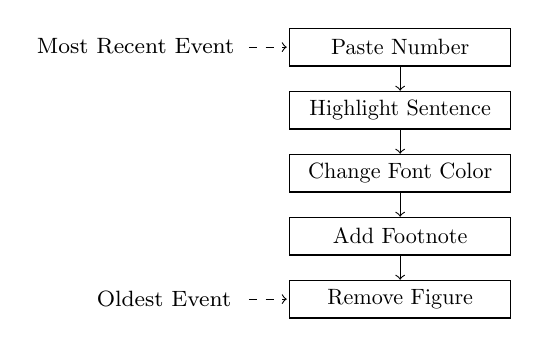
\begin{tikzpicture}[
  scale=.8,
  stacknode/.style={rectangle, draw, minimum width=1.5cm, minimum height=0.6cm, minimum width=3.5cm, text centered,scale=.8},
  dashedarrow/.style={->, dashed}
]

% Stack nodes
\node[stacknode] (top) at (0, 0) {Paste Number};
\node[stacknode] (node1) at (0, -1) {Highlight Sentence};
\node[stacknode] (node2) at (0, -2) {Change Font Color};
\node[stacknode] (node3) at (0, -3) {Add Footnote};
\node[stacknode] (bottom) at (0, -4) {Remove Figure};

% Arrows
\draw[->] (top.south) -- (node1.north);
\draw[->] (node1.south) -- (node2.north);
\draw[->] (node2.south) -- (node3.north);
\draw[->] (node3.south) -- (bottom.north);

% Line of text and dashed arrow
\draw[dashedarrow] (-2.4, 0) -- (-1.8, 0);
\node[align=center] at (-4.2, 0.025) {\footnotesize{}Most Recent Event};

\draw[dashedarrow] (-2.4, -4) -- (-1.8, -4);
\node[align=center] at (-3.75, -4) {\footnotesize{}Oldest Event};

\end{tikzpicture}
\end{center}
\caption{Example of ``Undo'' Event Stack in Text-Editing Program}
\label{fig:stackundo}
\end{figure}

\subsubsection*{\ttt{Queue} Interface}
Imagine you are in line at an amusement park for the most intense roller coaster in the world. 
Another, perhaps more generic term for a ``line'' is a \emph{queue}\index{queue}.
In this metaphor, riders enqueue the line at the back and board the roller coaster (and hence dequeue from the line) at the front. 

What we have described is a practical example of the queue data structure. 
In a queue, elements are enqueued, or inserted, onto the back of the queue, and are dequeued, or removed, from the front. 
Queues operate on the principle of first-in-first-out, or FIFO\index{first-in-first-out}. 
The implementation of a queue data structure may contain different names for their operations, but at their core should contain operations for inserting an element to the back of the queue (e.g., \textsc{enqueue}\index{enqueue}) and removing an element from the front of the queue (e.g., \textsc{dequeue}\index{dequeue}). 

Like the operations of a stack, \textsc{enqueue} and \textsc{dequeue} are also constant-time, since we store references to the front and rear elements of a queue. 
Queues, consequently, share similar drawbacks to stacks in that elements are not randomly accessible, i.e., we only know what exists at the front and rear of a queue instantaneously. 
Figure~\ref{fig:printerqueue} demonstrates the task queue of a printer, which has a sequence of files to print, one after another.

\begin{figure}[ht]
\begin{center}
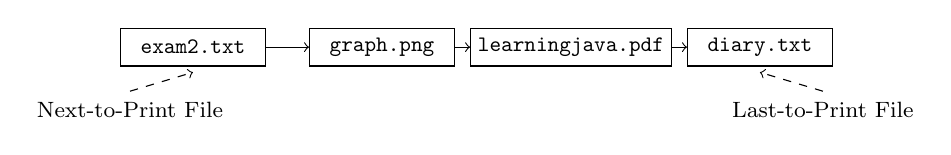
\begin{tikzpicture}[
    scale=.8,
  queuenode/.style={rectangle, draw, minimum width=1.5cm, minimum height=0.6cm, minimum width=2.3cm, text centered,scale=.8},
  dashedarrow/.style={->, dashed}
]

% Queue nodes
\node[queuenode] (front) at (0, 0) {\texttt{exam2.txt}};
\node[queuenode] (node1) at (3, 0) {\texttt{graph.png}};
\node[queuenode] (node2) at (6, 0) {\texttt{learningjava.pdf}};
\node[queuenode] (node3) at (9, 0) {\texttt{diary.txt}};

% Arrows
\draw[->] (front.east) -- (node1.west);
\draw[->] (node1.east) -- (node2.west);
\draw[->] (node2.east) -- (node3.west);

\draw[dashedarrow] (-1, -.7) -- (0, -.4);
\node[align=center] at (-1, -1) {\footnotesize{}Next-to-Print File};

\draw[dashedarrow] (10, -.7) -- (9, -.4);
\node[align=center] at (10, -1) {\footnotesize{}Last-to-Print File};

\end{tikzpicture}
\end{center}
\caption{Example of Printer Task Queue}
\label{fig:printerqueue}
\end{figure}

Unfortunately and inconveniently, there is no \ttt{Queue} class in Java. 
Instead, \texttt{Queue} is an \emph{interface}\index{interface} that other classes implement whose structure models the behavior of a queue. 
To create a first-in-first-out queue data structure, we initialize a variable to be a \texttt{Queue}, then instantiate it as a \texttt{LinkedList}. 
Thankfully, the \texttt{LinkedList} class contains all the relevant methods for operating a FIFO-based queue.

\begin{verbnobox}[\small]
Queue<Integer> q = new LinkedList<>();
\end{verbnobox}

Treating \texttt{q} as a queue rather than a linked list is easy thanks to the methods supplied by the \texttt{LinkedList}\index{\ttt{LinkedList}} implementation. 
Figure~\ref{fig:queues} shows some of these handy methods. 

\begin{figure}[tp]
  \small
  \begin{tcolorbox}[title=Java Queue]
    A \emph{Queue}\index{queue}\index{\ttt{Queue}} is a first-in-first-out (FIFO) sequential data structure where each element is linked to the element immediately after.
    \vspace{2ex}
  \begin{description}
    \item [\ttt{Queue<$T$> $Q=$ new LinkedList<>$()$}] creates a \ttt{Queue} of type $T$, named $Q$.
     \item [\ttt{void $Q$.addLast$(e)$}] adds $e$ to the end of $Q$, placing it at the end of the queue structure.
     \item [\ttt{$T$ $Q$.poll$()$}] returns and removes the element from the front of the queue.
     \item [\ttt{$T$ $Q$.peek$()$}] returns the front-most element in the queue.
    \item [\ttt{int $Q$.size$()$}] returns the number of logical elements in the queue.
  \end{description}
\end{tcolorbox}
  \caption{Useful \ttt{Queue}-based Methods.}
  \label{fig:queues}
\end{figure}

\subsubsection*{\ttt{PriorityQueue} Class}
\begin{figure}[tp]
  \small
  \begin{tcolorbox}[title=Java PriorityQueue]
    A \emph{Priority queue}\index{priority queue} is a rank/score-based data structure wherein the ordering of elements is determined by either their natural ordering or a \ttt{Comparator}.
    \vspace{2ex}
  \begin{description}
    \item [\ttt{PriorityQueue<$T$> $PQ=$ new PriorityQueue<>$(c)$}] creates a \ttt{PriorityQueue} of type $T$, named $PQ$, with a \ttt{Comparator} $c$ that is used to compare objects of type $T$ within the priority queue.
     \item [\ttt{void $PQ$.add$(e)$}] inserts $e$ into $PQ$, whose position in the priority queue depends on the currently-existing elements.
     \item [\ttt{$T$ $PQ$.poll$()$}] returns and removes the element with the highest priority.
     \item [\ttt{$T$ $PQ$.peek$()$}] returns the element with the highest priority.
    \item [\ttt{int $PQ$.size$()$}] returns the number of logical elements in the priority queue.
  \end{description}
\end{tcolorbox}
  \caption{Useful \ttt{PriorityQueue}-based Methods.}
  \label{fig:priorityqueues}
\end{figure}

\emph{Priority queues}\index{priority queues} are the final sequential data structure that we will discuss from the Collections API\@. 
Though, placing priority queues in this section feels a bit disingenuous because, while priority queues have an ordering in their underlying data structure, saying that elements correspond to an index is a misnomer. 
Priority queues, as the name suggests, rank items in the queue by a score called the \emph{priority}\index{priority}. 
Elements with the highest priority are at the ``front'' of the priority queue. 
Inserting elements into a priority queue potentially alters the positioning of preexisting elements.

Priority queues base priority on one of two contributing factors: either the \emph{natural ordering}\index{natural ordering} of elements, or a \emph{comparator object}\index{comparator object}. 
The natural ordering of elements is straightforward: natural ordering for numbers is their standard numeric ordering from least to greatest. 
For strings, the natural ordering is their lexicographical ordering. 
Natural ordering, however, are not as interesting as comparators, which we will now discuss.

A \emph{comparator}\index{comparator} is a way of comparing two arbitrary ``things.'' 
Whether these ``things'' are numbers (i.e., the wrapper classes), strings, or another kind of object, we can define custom ways of comparing \emph{any} non-primitive datatype.

\myexample{Let's design a \ttt{Comparator}\index{\ttt{Comparator}} for prioritizing strings that start with the lowercase letter \ttt{\q{p}\q{}}}.
Comparators are constructed like all other objects via \ttt{new}, but something interesting about their implementation is that we must specify \emph{how} to compare two objects. 
Therefore, when we create a new instance of \ttt{Comparator}, we must also override its \ttt{compare} method. 
The \ttt{compare} method's signature varies based on the parameterized type provided to the comparator, but since we want to compare strings, we should declare it as follows:

\begin{lstlisting}[language=MyJava]
import java.util.Comparator;
import java.util.PriorityQueue;

class PriorityQueueByP {

  /**
   * Returns a priority queue that prioritizes strings 
   * that start with `p'.
   * @return priority queue instance.
   */
  static PriorityQueue<String> priorityByP() {
    Comparator<String> c = new Comparator<>(
      @Override
      public int compare(String s1, String s2) { 
        // TODO.
      }
    );
  }
}
\end{lstlisting}

We now must describe how we want to compare~\ttt{s1} and~\ttt{s2} to achieve our goal.
Strangely enough, if we want to say that~\ttt{s1} has a higher priority than~\ttt{s2}, we must return a negative value, similar to the natural ordering of strings (this idea extends to any type we wish to compare, however). 
Fortunately, this is not as strange once we understand \emph{why} the negative value is required. 
A value of~$-1$ comes prior to~$1$ when placing numbers in ascending order. 
Consequently, when comparing an arbitrary value~$t_1$ against~$t_2$, to say that~$t_1$ comes before~$t_2$, we return a negative integer. Conversely, to say that~$t_1$ comes after~$t_2$, we return a positive number.

Let's perform a case analysis on the input strings. 
If both provided strings are non-empty, we retrieve their first character. 
If both start with \ttt{'p'}, then their ordering depends on a standard lexicographical comparison of the rest of the strings. 
If the first character of~$s_1$ is \ttt{'p'}, however, we return~$-1$ to designate that~$s_1$ has a higher priority than~$s_2$. 
Conversely, if~$s_2$ starts with \ttt{'p'}, then we return~$1$ to designate the opposite. 
If neither start with~$p$, then again we perform a lexicographical comparison on the entire strings. 
Algorithm~\ref{alg:pseudocodepriority} displays the pseudocode for the comparator, but as we will see, we can translate this, verbatim, into Java syntax. 
The last line of \ttt{priorityByP} instantiates a new \ttt{PriorityQueue}\index{\ttt{PriorityQueue}} whose constructor receives the \ttt{Comparator}\index{\ttt{Comparator}} that we just designed. 

\begin{algorithm}[H]
\begin{algorithmic}
\Procedure{Compare}{$s_1$, $s_2$}
    \If {$s_1$ \textbf{and} $s_2$ are non-empty}
        \State $c_1 \gets \textbf{First}(s_1)$
        \State $c_2 \gets \textbf{First}(s_2)$
        \If {$c_1$ is `p' \textbf{and} $c_2$ is `p'}
            \State $xs_1 \gets s_1$\emph{.substring(1)}
            \State $xs_2 \gets s_2$\emph{.substring(1)}
            \State \Return $xs_1$\emph{.compareTo}$(xs_2)$
        \ElsIf {$c_1$ is `p'}
            \State \Return $-1$
        \ElsIf {$c_2$ is `p'}
            \State \Return $1$
        \Else
            \State \Return $s_1$\emph{.compareTo}$(s_2)$
        \EndIf
    \Else
        \State \Return $s_1$\emph{.compareTo}$(s_2)$
    \EndIf
\EndProcedure
\end{algorithmic}
\caption{Pseudocode for Comparing Two Strings For `p' Priority}
\label{alg:pseudocodepriority}
\end{algorithm}

\begin{lstlisting}[language=MyJava]
import java.util.Comparator;
import java.util.PriorityQueue;

class PriorityQueueByP {

  static PriorityQueue<String> priorityByP() {
    Comparator<String> c = new Comparator<>() {
      @Override
      public int compare(String s1, String s2) {
        if (!s1.isEmpty() && !s2.isEmpty()) {
          char c1 = s1.charAt(0);
          char c2 = s2.charAt(0);
          if (c1 == 'p' && c2 == 'p') {
            return s1.substring(1).compareTo(s2.substring(1));
          } else if (c1 == 'p') {
            return -1;
          } else if (c2 == 'p') {
            return 1;
          } else {
            return s1.compareTo(s2);
          }
        } else {
          return s1.compareTo(s2);
        }
      }
    };
    return new PriorityQueue<String>(c);
  }
}
\end{lstlisting}

Let us add a few elements to a priority queue with our custom comparator to exemplify the idea. To add elements, we use \ttt{.add}, and to remove the element with the highest priority, we invoke \ttt{.poll}.

\begin{lstlisting}[language=MyJava]
import java.util.Comparator;
import java.util.PriorityQueue;

class PriorityQueueByP {

  static PriorityQueue<String> priorityByP() { /* Code hidden. */ }

  public static void main(String[] args) {
    PriorityQueue<String> pq1 = priorityByP();
    // Add a few values.
    pq1.add("pool"); pq1.add("peek"); pq1.add("hello"); pq1.add("barks");
    pq1.add("park"); pq1.add("pecking"); pq1.add("shrub");

    // Poll each from the queue and print them out.
    while (!pq1.isEmpty()) { System.out.println(pq1.poll()); }
  }
}
\end{lstlisting}

The output is as follows:

\begin{verbnobox}[\small]
park
pecking
peek
pool
barks
hello
shrub
\end{verbnobox}

With the provided comparator, \ttt{park} has the highest priority because it starts with \ttt{'p'} and has a substring that comes before the rest of those strings starting with \ttt{'p'}. 
The strings \ttt{pecking}, \ttt{peek}, and \ttt{pool} come next for similar reasons. 
Finally, none of the strings \ttt{barks}, \ttt{hello}, and \ttt{shrub} start with \ttt{'p'}, so we compare based on the strings themselves. 
The underlying implementation of \emph{how} the priority queue works and enforces ordering is beyond the scope of this textbook. 
Such details are reserved for a textbook or course on advanced data structures, which follows the course designed for the audience of this text.

\subsection{Set-Based Data Structures}
\emph{Sets} are unordered collections of non-duplicate elements. 
Does this definition sound familiar? 
It should; it perfectly mirrors the mathematical definition of a set. 
Java has a few nuances to its definition of sets that we will now see. 
We consider these data structures \emph{set-based} since they all rely on the ``no-duplicate'' philosophy.

\subsubsection*{\ttt{Set} Interface}
A \emph{Set}\index{set}\index{\ttt{Set}} in Java is an interface rather than a class. 
This is because Java has a hierarchy for differing implementations of sets. 
We will discuss three such implementations: \emph{HashSet}, \emph{TreeSet}, and \emph{LinkedHashSet}. 
While all three disallow duplicate elements, the latter two impose an ordering on their elements, which goes against the standard mathematical definition, but for practical reasons.

\subsubsection*{\ttt{HashSet} Class}
In the implementation of a \ttt{HashSet}\index{hash set}\index{\ttt{HashSet}}, the existence of objects in the set is determined by the \ttt{hashCode()} method of the objects, which computes their hash codes. 
These hash codes are used to decide in which `bucket' within the hash table an object should be placed. 
It's important, though, to note that hash codes are not used for comparing the equality of the content of objects. 
Unlike the \ttt{==} operator, which checks if two references point to the same object in memory, the respective \ttt{equals()} method is used to compare the actual content of the objects. 
When adding an object to a \ttt{HashSet}, if the hash code of the object matches the hash code of any existing object in the corresponding bucket, the \ttt{equals()} method is then used to check for actual content equality to ensure that no duplicate objects (in terms of content) are added to the set. 
In other words, two objects that are equal in terms of \ttt{equals()} must have the same hashcode, but the converse is not necessarily true. 
Anything more than these details goes beyond the scope of this textbook, but we will provide a small synopsis of hashable data structures.

A hashable data structure is most often designed as a hash table, which is similar to an array, where elements are stored. 
Hashable data structures are known for their fast lookup times, thanks to a \emph{hash function}\index{hash function}: a mathematical function used to compute the location to store a value in a hash table. 
Consider a hash function~$H(v)$, whose range is the set of integers~$[0, n)$, where~$n$ is the number of elements of the hash table. 
Running~$v$ (which is an arbitrary argument) through the hash function~$H$ returns an index of the hash table. 
Evaluating~$H$ is, in optimal conditions, a constant-time algorithm, hence determining value existence in a hash table also runs in constant-time. 
This begs the question of what happens if there exists an output of~$H$ such that~$H(v') = H(v)$, but $v' \neq v$. 
In subsequent computer science courses, students learn how to resolve \emph{hash collisions}\index{hash collisions} through techniques such as linear and quadratic probling, as well as chaining.\footnote{In Chapter~\ref{chapter-classes}, we will implement a simple hash table that uses chaining to resolve hash collisions.}
%The previous paragraph briefly discussed this through the `buckets' analogy and \ttt{equals}, but we will ignore such complexities and use hashable data structures at face value.  

Use hashsets when you do not care about element ordering or ``position'' in the set, and want to ensure no duplicates exist.
\begin{figure}[tp]
  \small
  \begin{tcolorbox}[title=Java Sets]
    A \emph{Set}\index{set}\index{\ttt{Set}} is a data structure of non-duplicate elements, with \ttt{HashSet} being the most common implementation/usage of sets.
    \vspace{2ex}
  \begin{description}
    \item [\ttt{Set<$T$> $S=$ new HashSet<>$()$}] creates a \ttt{HashSet} of type $T$, named $S$.
     \item [\ttt{boolean $S$.contains$(e)$}] returns whether or not $e$ is in the set $S$.
     \item [\ttt{boolean $S$.add$(e)$}] adds $e$ to the set $S$ only if it is not present. If $e$ is not in $S$, it returns \ttt{false}; otherwise, it returns \ttt{true}.
     \item [\ttt{boolean $S$.remove$(e)$}] removes $e$ from the set $S$ only if it is present. If $e$ is not in $S$, it returns \ttt{false}; otherwise, it returns \ttt{true}.
    \item [\ttt{int $S$.size$()$}] returns the number of logical elements in the set.
  \end{description}
\end{tcolorbox}
  \caption{Useful \ttt{Sets}-based Methods.}
  \label{fig:hashsets}
\end{figure}

\subsubsection*{\ttt{TreeSet} Class}
A \emph{TreeSet}\index{tree set}\index{\ttt{TreeSet}} is a set with determined order, either by the natural ordering of the elements or one defined by a \ttt{Comparator}, similar to a priority queue. 
All methods in a \ttt{Set} are, definitionally, implemented by a \ttt{TreeSet}.

\subsubsection*{\ttt{LinkedHashSet} Class}
A \emph{LinkedHashSet}\index{linked hash set}\index{\ttt{LinkedHashSet}} is a set with an ordering based on the insertion order of the elements. 
All methods in a \ttt{Set} are, definitionally, implemented by a \ttt{LinkedHashSet}.

\myexample{The canonical usage of a set is to remove duplicates from a list.} 
Indeed, let's design the \ttt{removeDuplicatesList} method that receives a list of integers and returns a new list without any duplicates. 
We will add a postcondition requirement that the output order of the integers must match the input order. 
To solve this problem, we will create an auxiliary linked hash set data structure, add all elements from the list into the set, then add those values from the set to a new list. 
When adding a value into a set, if it already exists, it is not re-added.

%\enlargethispage{4\baselineskip}
\begin{lstlisting}[language=MyJava]
import static Assertions.assertAll;
import static Assertions.assertEquals;

import java.util.List;

class RemoveDuplicatesListTester {

  @Test
  void testRemoveDuplicatesList() {
    assertAll(
      () -> assertEquals(List.of(), 
              removeDuplicatesList(List.of())),
      () -> assertEquals(List.of(1, 2, 3, 4), 
              removeDuplicatesList(List.of(1, 1, 2, 2, 3, 3, 4, 4))),
      () -> assertEquals(List.of(3, 1, 4), 
              removeDuplicatesList(List.of(3, 1, 1, 3, 4, 4, 3, 4))));
  }
}
\end{lstlisting}

\begin{lstlisting}[language=MyJava]
import java.util.List;
import java.util.ArrayList;
import java.util.Set;
import java.util.LinkedHashSet;

class RemoveDuplicatesList {

  /**
   * Removes duplicates from a list of integers.
   * @param ls - list of integers.
   * @return new list without duplicates.
   */
  static List<Integer> removeDuplicatesList(List<Integer> ls) {
    List<Integer> newLs = new ArrayList<>();
    Set<Integer> set = new LinkedHashSet<>();
    for (int x : ls) { set.add(x); }
    for (int x : s) { newLs.add(x); }
    return newLs;
  }
}
\end{lstlisting}

\myexample{Suppose we want to find all common elements shared between two linked lists of elements, which are unordered.} 
Let's design the \ttt{commonValues} method that, when given two linked lists of integers, returns a sorted-ordered list of the values that occur in both lists. 
We should not count values twice, e.g., if \ttt{2} occurs twice in the first list, then the resulting output list should only contain one occurrence of \ttt{2}. 
Let's take advantage of a tree set to store the common values in order, and then add those values to a new linked list.

%\enlargethispage{2\baselineskip}
\begin{lstlisting}[language=MyJava]
import static Assertions.assertAll;
import static Assertions.assertEquals;

import java.util.List;
import java.util.LinkedList;
import java.util.Set;
import java.util.TreeSet;

class CommonValuesTester {

  @Test
  void testCommonValues() {
    assertAll(
      () -> assertEquals(List.of(), 
                         commonValues(List.of(),
                                      List.of(5, 4, 3, 2, 1))),
      () -> assertEquals(List.of(), 
                         commonValues(List.of(10, 20, 30, 40, 50),
                                      List.of(5, 4, 3, 2, 1))),
      () -> assertEquals(List.of(1, 3, 4), 
                         commonValues(List.of(2, 4, 1, 3, 5, 6),
                                      List.of(1, 4, 3, 10, 20))),
      () -> assertEquals(List.of(-2, 0, 2), 
                         commonValues(List.of(2, -2, 0, 0, -2, 2),
                                      List.of(-2, 2, 0))));
  }
}
\end{lstlisting}

\begin{lstlisting}[language=MyJava]
import java.util.List;
import java.util.LinkedList;
import java.util.Set;
import java.util.TreeSet;

class CommonValuesTester {

  /**
   * Finds all common values between two linked lists of integers.
   * @param ls1 - first linked list.
   * @param ls2 - second linked list.
   * @return list of (distinct) common values.
   */
  static List<Integer> commonValues(LinkedList<Integer> ls1, 
                                    LinkedList<Integer> ls2) {
    Set<Integer> set = new TreeSet<>();
    for (int x : ls1) {
      if (ls2.contains(x)) { 
        set.add(x); 
      }
    }
    List<Integer> newLs = new LinkedList<>();
    newLs.addAll(set);
    return newLs;
  }
}
\end{lstlisting}

\myexample{We are given an array of numbers from~$1$ to~$n$, where one number is missing and one is duplicated. 
Let's design the \ttt{findDupMissing} method that returns an array of two elements: the first of which is the missing number and the second of which is the duplicate value. 
It makes sense to use a \ttt{TreeSet} since, that way, we can store the numbers in order and find out which one is omitted through one traversal, and find the only duplicate.}


\begin{lstlisting}[language=MyJava]
import static Assertions.assertAll;
import static Assertions.assertArrayEquals;

class FindDupMissingTester {

  @Test
  void testFindDupMissing() {
    assertAll(
      () -> assertArrayEquals(new int[]{2, 3}, 
              findDupMissing(new int[]{1, 3, 3, 4})),
      () -> assertArrayEquals(new int[]{5, 1}, 
              findDupMissing(new int[]{8, 1, 4, 1, 3, 2, 6, 7})),
      () -> assertArrayEquals(new int[]{6, 7}, 
              findDupMissing(new int[]{3, 2, 7, 7, 4, 5, 1})));
  }
}
\end{lstlisting}

%\enlargethispage{-1\baselineskip}
\begin{lstlisting}[language=MyJava]
import java.util.Set;
import java.util.TreeSet;

class FindDupMissing {

  /**
   * Finds a duplicate number and a missing number from 
   * an array of numbers within a specific interval.
   * @param A - array of integers where each number is in [1, n],
   *            with one missing and one duplicate.
   * @return two-element array where [0] is the missing number
   *         and [1] is the duplicate number.
   */
  static int[] findDupMissing(int[] A) {
    Set<Integer> set = new TreeSet<>();
    int[] res = new int[2];
    // Add the values to the set and find the duplicate one.
    for (int x : A) {
      if (set.contains(x)) { res[1] = x; } 
      else { set.add(x); }
    }

    // Now find the missing number.
    int prev = 0;
    for (int x : set) {
      if (x != prev + 1) {
        res[0] = prev + 1;
        break;
      } else {
        prev = x;
      }
    }
    return res;
  }
}
\end{lstlisting}

\subsection{Dictionary-Based Data Structures}
Dictionaries map elements from one type~$K$ to elements of another type~$V$. The types~$K$ and~$V$ do not necessarily need to be distinct. 

\subsubsection*{\ttt{Map} Interface}
Java has an interface called \ttt{Map}\index{map}\index{\ttt{Map}} rather than a class because, like sets, there is a hierarchy for differing implementations of maps. 
We will discuss three: \emph{HashMap}, \emph{TreeMap}, and \emph{LinkedHashMap}.
Maps contain keys and values; the keys are mapped to values in the map. 
A key/value pairing is called an \emph{entry}\index{entry}, or an \emph{association}\index{association}.
Maps cannot contain duplicate keys, because it would be ambiguous to have two identical keys mapping to different values.

\subsubsection*{\ttt{HashMap} Class}
\emph{HashMaps}\index{hash map}\index{\ttt{HashMap}} base existence of keys in the map by their hashcode and a hash table, identical to a hash set. 
For a greater detail of how hashable data structures work, please refer to the previous subsection.

\begin{figure}[tp]
  \small
  \begin{tcolorbox}[title=Java Maps]
    A \emph{Map}\index{map} is a dictionary-based data structure wherein we map \emph{keys} to \emph{values}, with \ttt{HashMap} being the most common implementation/usage of maps.
    \vspace{2ex}
  \begin{description}
    \item [\ttt{Map<$K, V$> $M=$ new HashMap<>()}] creates a \ttt{HashMap} named $M$ whose keys are of type $K$ and whose values are of type $V$. Namely, the keys map to the values.
     \item [\ttt{$M$.containsKey$(k)$}] returns whether or not $k$ is a key in the map $M$.
     \item [\ttt{void $M$.put$(k, v)$}] maps the key $k$ to the value $v$ in $M$.
     \item [\ttt{$V$ $M$.get$(k)$}] returns the value associated with $k$ in $M$, or \ttt{null} if $k$ has no association.
     \item [\ttt{$V$ $M$.getOrDefault($k$, $x$)}] returns the value associated with $k$ in $M$, or $x$ if $k$ does not have an association.
    \item [\ttt{int $M$.size$()$}] returns the number of logical elements in the set.
    \item [\ttt{Set<$K$> keySet$()$}] returns a set of the keys in the map.
  \end{description}
\end{tcolorbox}
  \caption{Useful \ttt{Map}-based Methods.}
  \label{fig:hashmap}
\end{figure}

\subsubsection*{\ttt{TreeMap} Class}
A \emph{TreeMap}\index{tree map}\index{\ttt{TreeMap}} is a map with a determined order, either by a natural ordering of the keys or that defined by a comparator. 
All methods in \texttt{Map} are, definitionally, implemented by a \texttt{TreeMap}.

\subsubsection*{\ttt{LinkedHashMap} Class}
A \emph{LinkedHashMap}\index{linked hash map}\index{\ttt{LinkedHashMap}} is a map with an ordering based on the insertion order of the key/value pairs. 
All methods in a \ttt{Map} are, definitionally, implemented by a \ttt{LinkedHashMap}.

\myexample{Perhaps one of the most common use cases for a dictionary-based data structure is to compute the frequency, or count, of some values.} 
Suppose we want to design the \ttt{mode} method that, when given a list of integers, returns the mode(s), i.e., the most-frequent value(s). 
We can use a map to keep track of the numbers seen so far, which are the keys, and their respective frequencies being the values. 
Because a list of numbers may have multiple modes, we will need to use a three-step algorithm:

%\enlargethispage{4\baselineskip}
\begin{enumerate}
  \item Compute the frequencies of each number.
  \item Find the highest frequency.
  \item Find all numbers that match this frequency.
\end{enumerate}

Traversing over a map is straightforward: we obtain a \emph{key set}\index{key set}, which is a set of the keys in a map, and each corresponding value is retrieved via one call to the \ttt{.get} method.

\begin{lstlisting}[language=MyJava]
import static Assertions.assertAll;
import static Assertions.assertEquals;

import java.util.List;
import java.util.Set;

class ComputeModeTester {

  @Test
  void testMode() {
    assertAll(
      () -> assertEquals(Set.of(), mode(List.of())),  
      () -> assertEquals(Set.of(3), mode(List.of(4, 5, 2, 3, 3, 4, 3))),
      () -> assertEquals(Set.of(2, 3), mode(List.of(2, 3, 2, 3, 3, 2))),
      () -> assertEquals(Set.of(2), mode(List.of(2, 2, 2, 2, 2, 2, 2))));
  }
}
\end{lstlisting}

%\enlargethispage{5\baselineskip}
\begin{lstlisting}[language=MyJava]
import java.util.HashMap;
import java.util.HashSet;
import java.util.List;
import java.util.Map;
import java.util.Set;

class ComputeMode {

  /**
   * Computes the mode of a list of numbers, which is the most-frequent
   * value, or values.
   * @param ls - list of numbers.
   * @return set of mode values, if they exist.
   */
  static Set<Integer> mode(List<Integer> ls) {
    if (ls.isEmpty()) { return new HashSet<>(); } 
    else {
      // First, compute the frequencies.
      Map<Integer, Integer> frequencies = new HashMap<>();
      for (int v : ls) {
        if (!frequencies.containsKey(v)) {
          frequencies.put(v, 1);
        } else {
          frequencies.put(v, frequencies.get(v) + 1);
        }
      } 

      // Find the highest frequency.
      int highestFreq = -1;
      for (int k : frequencies.keySet()) {
        highestFreq = Math.max(highestFreq, frequencies.get(k));
      }

      // Now, find the values that match that frequency.
      return frequencies.keySet()
                        .stream()
                        .filter(k -> frequencies.get(k) == highestFreq)
                        .collect(Collectors.toSet());
    }
  }
}
\end{lstlisting}

\myexample{Let's design the \ttt{sharesFirstChar} method that, when given an array of strings, returns a \ttt{Map<Character, Set<String>{>}} such that each alphabetized character maps to a set of alphabetized strings that start with that character.} 
We will further assume a case-insensitive mapping. 
Consider the following input and output example:

\begin{verbnobox}[\small]
sharesFirstChar(["she", "sells", "sea", "shells", "by", "the", "sea"])
  => [<'b' : {"by"}>, 
      <'s' : {"sea", "sells", "she", "shells"}>
      <'t' : {"the"}>]
\end{verbnobox}

Because we want both the sets and maps to be alphabetized, the use of a \ttt{TreeSet} and \ttt{TreeMap} is appropriate. 
So, we will first traverse over the input list and instantiate a map whose keys are the first letters of each word, and whose value is a new instance of a \ttt{TreeSet}. 
We then populate the sets via a second traversal over the list.

\begin{lstlisting}[language=MyJava]
import static Assertions.assertAll;
import static Assertions.assertEquals;

import java.util.List;
import java.util.Map;
import java.util.Set;
import java.util.TreeMap;

class ShareFirstCharacterTester {
  
  @Test
  void testShareFirstChar() {
    Map<Character, Set<String>> exp1 = new TreeMap<>();
    assertEquals(exp1, shareFirstChar(List.of()));

    Map<Character, Set<String>> exp2 = new TreeMap<>();
    exp2.put('b', new TreeSet<>());
    exp2.put('s', new TreeSet<>());
    exp2.put('t', new TreeSet<>());
    exp2.get('s').addAll(Set.of("she", "sells", "sea", "shells"));
    exp2.get('t').addAll(Set.of("the"));
    exp2.get('b').addAll(Set.of("by"));
    assertEquals(exp2, 
                 shareFirstChar(List.of("she", "sells", "sea", "shells", 
                                        "by", "the", "sea")));
  }
}
\end{lstlisting}

%\enlargethispage{4\baselineskip}
\begin{lstlisting}[language=MyJava]
import java.util.HashMap;
import java.util.List;
import java.util.Map;
import java.util.Set;
import java.util.TreeSet;

class ShareFirstCharacter {

  /**
   * Returns a map whose keys are the first characters of the strings
   * and whose values are sets of strings that start with that character.
   * @param ls - list of strings.
   * @return map of sets of strings.
   */
  static Map<Character, Set<String>> shareFirstChar(List<String> ls) {
    Map<Character, Set<String>> M = new HashMap<>();
    // Populate the map with the initial TreeSets.
    for (String s : ls) {
      char lc = Character.toLowerCase(s.charAt(0));
      if (!M.containsKey(lc)) {
        M.put(lc, new TreeSet<>());
      }
    }

    // Add the strings to each set.
    for (String s : ls) {
      M.get(Character.toLowerCase(s.charAt(0))).add(s);
    }
    return M;
  }
}
\end{lstlisting}

\myexample{Let's design the \ttt{firstUniqueDigit} method that, when given a string, returns the first non-repeated digit.} 
If there is no non-repeated digit, then return the empty string. 
Because we care about the insertion order, we should use a \ttt{LinkedHashMap} whose keys are characters in the string and whose values are frequency counts. 
The idea is to count the frequency of each (digit) character, then traverse over the linked map and find the first key whose (value) frequency is one. 
Because we now understand how to combine \ttt{get} and \ttt{put} to insert and increment frequency counts, we will instead opt to use \ttt{getOrDefault}, which removes the need for the conditional.\footnote{This problem is similar to one created by \ttt{frew@mclean.com} on \ttt{codingbat.com}. Thanks!}


\begin{lstlisting}[language=MyJava]
import static Assertions.assertAll;
import static Assertions.assertEquals;

class FirstUniqueDigitTester {

  @Test
  void testFirstUniqueDigit() {
    assertAll(
      () -> assertEquals("3", firstUniqueDigit("1211312121")),
      () -> assertEquals("2", firstUniqueDigit("0099828776")),
      () -> assertEquals("", firstUniqueDigit("11223344")));
  }
}
\end{lstlisting}

%\enlargethispage{2\baselineskip}
\begin{lstlisting}[language=MyJava]
import java.util.HashMap;
import java.util.Map;

class FirstUniqueDigit {

  /**
   * Returns the first unique digit in a string, as a string. 
   * If there is no unique digit, then the empty string is returned.
   * @param s - string.
   * @return first unique digit as a string.
   */
  static String firstUniqueDigit(String s) {
    Map<Character, Integer> M = new LinkedHashMap<>();
    // Count the frequency of each digit
    for (int i = 0; i < s.length(); i++) {
      String c = s.substring(i, i + 1);
      if (Character.isDigit(c.charAt(0))) {
        M.put(c.charAt(0), M.getOrDefault(c.charAt(0), 0) + 1);
      }
    }

    // Find the first unique letter.
    for (char c : M.keySet()) {
      if (M.get(c) == 1) {
        return String.valueOf(c);
      }
    }
    return "";
  }
}
\end{lstlisting}

\myexample{One final example that we will consider is the \ttt{nthMostFrequentChar} method that, when given a string~$s$ and an integer~$n$, returns the~$n^\text{th}$ most frequent character in the string, or \ttt{null} if there is no such character.} 
If there are multiple characters that share the same position, we return the first one in terms of lexicographical ordering.

For example, consider the string \ttt{"abbabdcaadaababcdcc"} and~$n=3$. 
The most frequent characters are \ttt{\q{}a\q{}, \q{}b\q{}, \q{}c\q{}}, in that order.
So, the third most frequent character is \ttt{\q{}c\q{}}.

Another example is the string \ttt{"aabbcc"} and~$n=2$. 
The most frequent characters are \ttt{\q{}a\q{}, \q{}b\q{}, \q{}c\q{}}, in that order, but all three characters share a frequency of two, meaning they are all equally frequent. 
In this case, we return the empty string.

A third example is the string \ttt{"aaaabccccc"} and~$n=2$. 
The most frequent characters are \ttt{\q{}c\q{}, \q{}a\q{}, \q{}b\q{}}, in that order.
So, the second most frequent character is \ttt{\q{}a\q{}}.

First, we will count the frequency of each character, then use a \ttt{PriorityQueue} to store the characters in order of their frequency from greatest to least. 
We will then remove the first~$n-1$ characters from the priority queue, and return the first character of the remaining queue. 
This approach may raise some eyebrows, because if the frequency is the value in a map, how can we construct a comparator? 
In other circumstances, one needs access to a particular key to obtain its corresponding value. 
In this instance, though, we can generate the \emph{entry set} for the map of characters to frequencies, which is a set of \ttt{Map.Entry<K, V>} objects, where~$K$ is the key type and~$V$ is the value type. 
Our priority queue comparator receives two such entries~$e$ and~$f$, and performs the following comparison:

\begin{itemize}
  \item If $e_k \neq f_k$, return $f_v - e_v$.
  \item Else, return the lesser of $e_k$ and $f_k$.
\end{itemize}

We know that~$K$ is \ttt{Character} and~$V$ is \ttt{Integer} representing the characters mapped to their frequencies. 
To retrieve the key and value from an \ttt{Map.Entry} object, we use the \ttt{getKey()} and \ttt{getValue()} methods respectively. 

\begin{lstlisting}[language=MyJava]
import static Assertions.assertAll;
import static Assertions.assertEquals;

class NthMostFrequentCharTester {

  @Test
  void testNthMostFrequentChar() {
    assertAll(
      () -> assertEquals("a", nthMostFrequentChar("abacab", 1)),
      () -> assertEquals("d", nthMostFrequentChar("aaaadddcccccbbee", 3)),
      () -> assertEquals("q", nthMostFrequentChar("ppqrrss", 2)),
      () -> assertEquals(null, nthMostFrequentChar("aabbccdd", 2)));
  }
}
\end{lstlisting}

%\enlargethispage{8\baselineskip}
\begin{lstlisting}[language=MyJava]
import java.util.Comparator;
import java.util.HashMap;
import java.util.Map;
import java.util.PriorityQueue;

class NthMostFrequentChar {

  /**
   * Given a string, returns the nth most 
   * frequent character in that string.
   * @param s - string to examine.
   * @param n - int n >= 0.
   * @return the nth most frequent character as 
   *         a String or null if nonexistent.
   */
  static String nthMostFrequentChar(String s, int n) {
    // Step 1: compute the frequencies.
    Map<Character, Integer> M = new HashMap<>();
    s.chars().forEach(c -> M.put(c, M.getOrDefault(c, 0))); 

    // Step 2: build the comparator.
    Comparator<Entry<Character, Integer>> cmp = new Comparator<>() {
      @Override
      public int compare(Map.Entry<Character, Integer> e, 
                         Map.Entry<Character, Integer> f) {
        if (e.getKey() != f.getKey()) {
          return Character.compare(e.getKey(), f.getKey());
        } else {
          return f.getValue() - e.getValue();
        }
      }
    };

    // Step 3: populate the priority queue with entry objects.
    PriorityQueue<Map.Entry<Character, Integer>> Q 
      = new PriorityQueue<>(cmp);
    M.entrySet().forEach(e -> Q.add(e));

    // Step 4: poll n - 1 items from the queue.
    while (!Q.isEmpty()) {
      n--;
      if (n == 0) { return String.valueOf(Q.peek().getKey()); } 
      else { Q.poll(); }
    }
    return null;
  }
}
\end{lstlisting}

\section{Iterators}
We know how to iterate, or traverse, over a simple data structure such as an array. 
The idea is to use a variable for the index and continuously increment it until we reach the upper bound of the array. 
Below is a simple example where we sum the elements of an array.

\begin{verbnobox}[\small]
static int sum(int[] arr) {
  int sum = 0;
  for (int i = 0; i < arr.size; i++) { sum += arr[i]; }
  return sum;
}
\end{verbnobox}

The problem is that not all data structures, as we have undoubtedly seen, are sequential; sets and maps are two examples of non-sequential data structures, so how do we traverse over those? 
One option is the enhanced-for loop, but as we will show later, this approach has its drawbacks, even though its syntax is straightforward. 
Stacks and queues are another example of data structures that are not necessarily sequential. 
\emph{Iterator} objects are one answer to the traversability problem. 
Iterators provide a mechanism for traversing over a data structure. 
Any data structure whose class definition implements \ttt{Iterator} must define at least two methods: \ttt{boolean hasNext} and \ttt{T next}, which determines whether we are at the end of the traversal, and retrieves the next element, respectively. 
Note that \ttt{T}, for the time being, simply means ``any type,'' and is related to type parameterization.
All of the Java collections implement \ttt{Iterator}, and we can retrieve the corresponding \ttt{Iterator} object via the \ttt{.iterator} method. 

Upon retrieving an iterator, we can use a \ttt{while} loop to continuously retrieve elements in the data structure until no more elements remain to be visited. 
The elements of the iterator are generated on-the-fly; only upon calling \ttt{next} is the value truly read from the data structure itself. 
Much like the rest of the Collections API, we must pass the parameterized type to the \ttt{Iterator} initialization, so that it knows what type to substitute for \ttt{T}.

\myexample{Let's use an iterator to traverse over a \ttt{LinkedHashSet}, whose element ordering is determined by their insertion order, meaning that the iterator should produce them in the order that they were inserted.}

%\enlargethispage{5\baselineskip}
\begin{lstlisting}[language=MyJava]
import static Assertions.assertAll;
import static Assertions.assertEquals;

import java.util.Set;
import java.util.LinkedHashSet;
import java.util.Iterator;

class IteratorTester {

  @Test
  void testIterator() {
    Set<Integer> lhs = new LinkedHashSet<>(Set.of(8, 90));
    Iterator<Integer> it = lhs.iterator();
    assertAll(
      () -> assertTrue(it.hasNext());
      () -> assertEquals(8, it.next()),
      () -> assertEquals(90, it.next()),
      () -> assertFalse(it.hasNext()));
  }
} 
\end{lstlisting}

Should we want to traverse over the data again, we need to instantiate another instance of the iterator, because there is no way to reset the ``position'' of an iterator; they are a kind of ``one-time use'' objects.

It should be stated that the enhanced \ttt{for} loop is nearly identical to the job of an \ttt{Iterator}, so a programmer may wonder why not use the former over the latter. 
Inside an enhanced \ttt{for} loop, the data structure in question is immutable, meaning that we cannot add, insert, remove, or change elements. 
On the other hand, iterators allow structural modification. 
We would recommend not altering the data structure while traversing, even if it is permissible by Java, because doing so can produce irksome bugs. 

\myexample{Let's now iterate over the \ttt{LinkedHashSet} using an enhanced \ttt{for} loop.} We can do so by placing the type on the left-hand side of the element declaration. 
Our test subtracts the elements from left-to-right.

\begin{lstlisting}[language=MyJava]
import static Assertions.assertEquals;

import java.util.Set;
import java.util.LinkedHashSet;

class EnhancedForLoopTester {

  @Test
  void testEnhancedForLoop() {
    Set<Integer> lhs = new LinkedHashSet<>();
    lhs.add(1); lhs.add(2); lhs.add(3); lhs.add(4);
    int diff = 0;
    for (Integer e : lhs) { 
      diff -= e; 
    }
    assertEquals(-10, diff);
  }
}
\end{lstlisting}

\myexample{Not only does the use of an enhanced \ttt{for} loop disallow structural modification, it also does not preserve the order of specific data structures.} 
For example, suppose we have a stack $S=[10, 20, 30, 40, 50]$, where~$50$ is the top of the stack. 
If we want to print each element of~$S$ without iterators or modifying the stack itself, the obvious option is to use an enhanced \ttt{for} loop. 
Unfortunately, this does not go as expected: it prints the elements in the order they are inserted, i.e., first-in-first-out. 
Intuitively, we may expect the program to output the values via last-in-first-out, i.e., $50, 40, 30, 20, 10$. 
What's worse is that its \ttt{Iterator} implementation also makes the glaring mistake. 
The solution proposed by Oracle is to instead use the \ttt{ArrayDeque} class, which is a type of \ttt{Deque} object.\footnote{A \emph{deque}, pronounced as `deck,' is a double-ended queue, meaning we can insert and remove elements from either the front or the rear.}\footnote{See the note listed on Oracle's \ttt{Stack} documentation: \url{https://docs.oracle.com/javase/8/docs/api/java/util/Stack.html}}

%\enlargethispage{-1\baselineskip}
\begin{lstlisting}[language=MyJava]
import java.util.Stack;
import java.util.Iterator;
import java.util.Deque;
import java.util.ArrayDeque;

class StackPrinter {

  public static void main(String[] args) {
    Stack<Integer> S = new Stack<>(List.of(10, 20, 30, 40, 50));

    // Enhanced for loop prints them "incorrectly!"
    // An Iterator also has this issue.
    // We get "10, 20, 30, 40, 50" separated by newlines.
    S.forEach(x -> System.out.println(x));

    Deque<Integer> D = new ArrayDeque<>(List.of(10, 20, 30, 40, 50));

    // An ArrayDeque corrects this problem.
    // We correctly get "50, 40, 30, 20, 10" separated by newlines.
    D.forEach(x -> System.out.println(x));
  }
}
\end{lstlisting}

\myexample{The unintuitive nature of the enhanced \ttt{for} loop and certain iterator behavior does not stop with stacks, unfortunately.}
Priority queues are also afflicted as a consequence of their implementation. 
Let's see what happens when we create a priority queue whose comparator prioritizes the string \ttt{"Joshua"} over all strings and makes the string \ttt{"Jack"} have the lowest priority. 
In other words, any occurrence of \ttt{"Joshua"} should come before all other strings in the priority queue, whereas any occurrence of \ttt{"Jack"} should come after all other strings in the priority queue. 
Any strings in between are ordered naturally, i.e., via lexicographical ordering.

%\enlargethispage{2\baselineskip}
\begin{lstlisting}[language=MyJava]
import java.util.List;
import java.util.PriorityQueue;
import java.util.Comparator;

class PriorityQueuePrinting {

  private static PriorityQueue<String> initPriorityQueue() {
    Comparator<String> S = new Comparator<>() {
      @Override
      public int compare(String s1, String s2) {
        // If Joshua comes first or Jack comes last, 
        // then s1 is prioritized.
        if (s1.equals("Joshua") || s2.equals("Jack")) { return -1; } 
        // If Jack comes first or Joshua comes last, 
        // then s2 is prioritized.
        else if (s1.equals("Jack") || s2.equals("Joshua")) { return 1; } 
        // All other strings take standard priority (natural ordering).
        else { return s1.compareTo(s2); }
      }
    };
    return new PriorityQueue(S);
  }

  public static void main(String[] args) {
    PriorityQueue<String> pq = initPriorityQueue();
    pq.add("Peter"); pq.add("Joshua"); pq.add("Gautam"); pq.add("Jane");
    pq.add("Jack"); pq.add("Ratan"); pq.add("Dharmik"); pq.add("Sakshi");

    // Prints a seemingly random order!
    for (String s : pq) { System.out.println(s); }

    // Uses Arrays to sort the elements according to the PQ's comparator.
    String[] elements = pq.toArray(new String[0]);
    Arrays.sort(elements, pq.comparator());
    System.out.println(Arrays.toString(elements));
  }
}
\end{lstlisting}

By traversing over the elements with an enhanced \ttt{for} loop, we notice that the elements are printed in a seemingly random order that does not obey our comparator. 
One solution here is to convert the priority queue to an array, sort the array using \ttt{Arrays.sort}, then print the contents of the array using \ttt{Arrays.toString}. 
Remember that, if we only pass the array itself to \ttt{println}, we see the hash code of the array is printed instead of its elements. 

One complication to concern ourselves with is how we convert the priority queue (or any collection) to an array using \ttt{.toArray(...)}. 
It receives an array of some type \ttt{T} and, if it is large enough to store all the elements of the collection, it is populated. 
Otherwise, an array of the same type \ttt{T} is returned. 
To summarize, if we want to convert the priority queue of strings into an array, we must pass \ttt{new String[0]} to the \ttt{.toArray} method. 
The returned array is then sorted and printed.\footnote{In the next section, we will discuss a much easier way to replicate \ttt{toArray} using a new collection type called \emph{streams}.} 

A final intricacy of conversion process is that we need to pass the comparator of the priority queue to \ttt{Arrays.sort}, otherwise it sorts the elements based on their natural ordering, which is certainly undesired. 
We do not have direct access to the comparator that we created in the \ttt{initPriorityQueue} method, but we can retrieve the comparator used by the priority queue via the priority queue \ttt{.comparator} method. 

\myexample{Gilmore and Kushagra are playing a game of ``pick the maximum.''}
The rules are that Gilmore removes the maximum value from a given list of numbers, then Kushagra does the same.
Kushagra then puts their number into another list, followed by Gilmore's number (okay, this isn't exactly a competitive game).
We want to see what the resulting list would be for a given input.
Let's design the \ttt{List<Integer> maximalMoves(List<Integer> ls)} method that, when given a list of numbers, and playing the game as aforementioned, returns the moves made by the players.
The naive approach is to traverse the list and remove the maximum element for each and every value. 
Unfortunately, this algorithm is terribly slow, being quadratic in the number of required iterations.
A more performant method is to add each item to a maximal priority queue (i.e., a priority queue whose comparator sorts items from greatest to least), withdraw two items at a time, and add them to the resulting list in the opposite order.
To create a comparator that uses ``greatest'' as the ``highest'' priority metric, we can use the \ttt{Collections.reverseOrder} method, which returns a comparator that sorts items in reverse order.

\begin{lstlisting}[language=MyJava]
import static Assertions.assertAll;
import static Assertions.assertEquals;

import java.util.List;
import java.util.PriorityQueue;
import java.util.Collections;

class MaximalMovesTester {

  @Test
  void testMaximalMoves() {
    assertAll(
      () -> assertEquals(List.of(), 
                         maximalMoves(List of())),
      () -> assertEquals(List.of(4, 5, 3, 2, 0, 1), 
                         maximalMoves(List.of(0, 1, 2, 3, 4, 5))),
      () -> assertEquals(List.of(45, 60, 35, 25, 45, 25, 10, 15, 5), 
                         maximalMoves(List.of(20, 40, 30, 25, 45, 
                                              25, 15, 10, 5, 60, 35))));
  }
}
\end{lstlisting}

\begin{lstlisting}[language=MyJava]
import java.util.List;
import java.util.PriorityQueue;

class MaximalMoves {

  /**
   * Given a list of numbers, returns the moves made by the players
   * @param ls - list of numbers.
   * @return list of moves.
   */
  static List<Integer> maximalMoves(List<Integer> ls) {
    PriorityQueue<Integer> pq = 
      new PriorityQueue<>(Collections.reverseOrder());
    pq.addAll(ls);
    List<Integer> moves = new ArrayList<>();
    // We will assume that the list has an even number of elements.
    for (int i = 0; i < ls.size() - 1; i += 2) {
      moves.add(pq.poll());
      moves.add(pq.poll());
    }
    return moves;
  }
}
\end{lstlisting}



\section{Streams}
\emph{Streams} are, in effect, a \emph{lazy} collection of ``things.'' 
By ``lazy,'' we mean to say that, if a result is not necessary nor requested, then it is not computed.

\myexample{Consider a situation where we invoke the \ttt{omega()} method, which is defined as an infinite loop, as the argument to the \ttt{foo} method, giving us \ttt{foo(omega())}.} 
In Java, all arguments are evaluated \emph{eagerly}, meaning that the arguments are evaluated before the method is applied.
Unfortunately for the caller of \ttt{foo}, the body thereof does not make use of~$x$, meaning we evaluate \ttt{omega()} for no reason whatsoever. 
This means that, because \ttt{omega} never terminates, \ttt{foo} similarly never returns a result.

\begin{verbnobox}[\small]
static int omega() {
  while (true) {}
  return 10;
}
\end{verbnobox}
\begin{verbnobox}[\small]
static int foo(int x) {
  return 5;
}
\end{verbnobox}

If Java supported \emph{lazy evaluation} for method calls, we would not have this problem.
Our discussion is not entirely driven by a desire for lazy evaluation, but rather the desire for easily-composable operations; lazy evaluation is a perk in that it allows us to design infinite data structures! 
An ``infinite'' data structure raises some important questions about how to store ``infinite'' data. 
Imagine that we want to compute a list that contains every positive even integer. We can represent this as the following inductive set:

\begin{align*}
    &0 \in S\\
    &\text{If } x \in S,\text{ then }x + 2 \in S
\end{align*}

Therefore,~$S$ is a set containing countably-infinite values. 
Implementing~$S$ in Java, as an \ttt{ArrayList}, might contain a \ttt{for} loop with a condition that we do not know how to solve! 
Because we do not know how many values to add, we may be tempted to design an infinite loop via \ttt{while (true)}, but then the loop never ends, and eventually the program runs out of memory due to adding values to the never-ending list. 
The solution, as we have suggested, is to use streams.\footnote{For those coming from another language such as Python, a stream is equivalent to a \emph{generator}.}


To create a stream of infinite data is to recreate our inductive set definition inside a \ttt{IntStream} instance and invoke the \ttt{iterate} static method.

\begin{verbnobox}[\small]
IntStream is = IntStream.iterate(0, x -> x + 2);
\end{verbnobox}

Let's explain this method, but to do so we must simultaneously introduce \emph{lambda expressions}. 
A lambda expression is an anonymous function, i.e., a function definition without a name. 
In the above code snippet, we define a function that receives a value~$x$ and returns~$x$ plus two. 
It would be identical to defining a \ttt{private static} method to add $2$ to some given integer, but we like lambda expressions due to their locality; it might come across as superfluous to design a method that is used in only one context. 
It is also possible to pass a \emph{method reference} instead of a lambda expression.

%\enlargethispage{4\baselineskip}
\begin{lstlisting}[language=MyJava]
import java.util.IntStream;

class PositiveEvens {

  private static int addTwo(int x) { return x + 2; }

  public static void main(String[] args) {
    IntStream is = IntStream.iterate(0, PositiveEvens::addTwo);
  }
}   
\end{lstlisting}

The \ttt{IntStream} instance declares a stream that, when requested/prompted, invokes and populates the stream. 
Because it is impossible to represent a truly infinite data structure in Java with modern computers, we need to limit how many values we want from this stream. 
Indeed, the \ttt{.limit} method computes exactly~$n$ elements from the stream. 
So, to compute the first ten elements of our $\emph{is}$ \ttt{IntStream}, we invoke \ttt{.limit(10)} on our $\emph{is}$ stream. 

\begin{lstlisting}[language=MyJava]
import java.util.IntStream;

class PositiveEvens {
  
  public static void main(String[] args) {
    IntStream is = IntStream.iterate(0, x -> x + 2).limit(10);
  }
}
\end{lstlisting}

Now, suppose we want to view these ten elements. 
Right now, they are consolidated to an \ttt{IntStream}, but we need to convert them to a list of sorts. 
The solution is to convert the values into a \ttt{Stream<Integer>} via \ttt{.boxed()}, and then to a list using the convenient \ttt{.toList()} method.

\begin{lstlisting}[language=MyJava]
import java.util.IntStream;
import java.util.List;

class PositiveEvens {
  
  public static void main(String[] args) {
    IntStream is = IntStream.iterate(0, x -> x + 2).limit(10);
    List<Integer> ls = is.boxed().toList();
    System.out.println(ls); // [0, 2, 4, 6, 8, 10, 12, 14, 16, 18]
  }
}
\end{lstlisting}

\myexample{Suppose we want a stream of infinitely repeating \ttt{"a"} strings.} 
We can easily create one via the \ttt{generate} method, which acts as the stream constructor, receiving a lambda expression to continuously generate new elements.

\begin{lstlisting}[language=MyJava]
import java.util.Stream;

class AGenerator {

  public static void main(String[] args) {
    Stream<String> as = Stream.generate(() -> "a");
    // ["a", "a", "a", "a", "a", "a", "a", "a", "a", "a"]
    System.out.println(as.limit(10).boxed().toList()); 
  } 
}
\end{lstlisting}

Again, it is important to understand what happens under the hood of a stream. 
Elements thereof only generate when we request them through some accessory means, e.g., \ttt{limit}. 
As we previously suggested, attempting to access an infinite stream (without a limit) causes the program to hang and eventually crash with an \ttt{OutOfMemoryError} error.

\myexample{Imagine we want to create a stream of all of the Fibonacci numbers.} 
The thing is, we eventually reach the~$32$-bit limit of the \ttt{int} datatype, so we should take advantage of the \ttt{BigInteger} class, allowing us to represent arbitrarily-large integers.\footnote{Worrying about \emph{how} the \ttt{BigInteger} class works for now is unnecessary as our current plan is to demonstrate stream properties.} 
Also, this time, we will design a method that returns the stream instance rather than creating one in the \ttt{main} method.

Here's what we need to do: let's use \ttt{iterate} to generate new values in the sequence. There is a slight problem in that the Fibonacci sequence has two starting (accumulator) values:~$0$ and~$1$. 
The issue is that \ttt{iterate} receives only one ``initializer'' value. 
To circumvent this predicament, we can pass an array that contains the current and ``next'' Fibonacci values. 
Inside the lambda expression, we receive an array of values, from which we compute the next Fibonacci number. 
Instead of using \ttt{IntStream}, however, we generalize to the \ttt{Stream} class, since our initial value(s) is not an integer.

\begin{lstlisting}[language=MyJava]
import static Assertions.assertEquals;
import static Assertions.assertArrayEquals;

import java.util.Stream;
import java.util.List;
import java.util.ArrayList;
import java.util.BigInteger;

class BigIntFibStreamTester {

  @Test
  void testBigIntFibStream() {
    // Get the stream, test ten values, 
    // make sure the lists are the same
    // length, then test each subarray.
    Stream<BigInteger[]> s = StreamExample.fibonacciStream();
    List<BigInteger[]> actualLs = s.limit(10).toList();
    List<BigInteger[]> expectedLs 
      = new ArrayList<>(
        List.of(new BigInteger[]{new BigInteger("0"), 
                                 new BigInteger("1")},
                new BigInteger[]{new BigInteger("1"), 
                                 new BigInteger("1")},
                ...));

    // Check each array of BigIntegers of the expected and actual.
    assertTrue(expectedLs.size() == actualLs.size());
    for (int i = 0; i < expectedLs.size(); i++) {
      assertArrayEquals(expectedLs.get(i), actualLs.get(i));
    }
  }
}
\end{lstlisting}

%\enlargethispage{-2\baselineskip}
\begin{lstlisting}[language=MyJava]
import java.util.Stream;
import java.util.BigInteger;

class BigIntFibStream {

  /**
   * Computes a stream of BigInteger values of the nth Fibonacci value.
   * @return stream containing arrays of the next sequential BigIntegers.
   */
  static Stream<BigInteger[]> fibonacciStream() {
    BigInteger[] vals = new BigInteger[]{new BigInteger("0"),
                                         new BigInteger("1")};
    return Stream.iterate(vals, v -> 
                          new BigInteger[]{v[1], v[0].add(v[1])});
  }
}
\end{lstlisting}

\begin{figure}[tp]
  \small
  \begin{tcolorbox}[title=Java Streams]
    A \emph{stream} is a lazy collection of elements that are computed only when requested.
    \vspace{2ex}
  \begin{description}
    \item [\ttt{int $S$.count$()$}] returns the number of elements in the stream.
    \item [\ttt{Stream<$T$> $S$.map$(f)$}] returns a new stream whose elements are the result of applying $f$ to each element of~$S$.
    \item [\ttt{Stream<$T$> $S$.filter$(p)$}] returns a new stream of values in $S$ that satisfy the predicate~$p$.
    \item [\ttt{$T$ $S$.reduce$(a, f)$}] returns the result of applying the binary function $f$ to each element of $S$, starting from $a$, which serves as the accumulator's initial value. The type of $a$ is $T$, which matches the elements of the stream.
    \item [\ttt{Stream<$T$> $S$.limit$(n)$}] returns a new stream containing the first $n$ elements of~$S$.
    \item [\ttt{Stream<$T$> $S$.skip$(n)$}] returns a new stream containing the elements of $S$ after the first~$n$.
    \item [\ttt{Optional<$T$> $S$.min/max$(c)$}] returns the minimum/maximum element of $S$ according to the comparator $c$. If $S$ is empty, returns \ttt{Optional.empty()}.
  \end{description}
\end{tcolorbox}
  \caption{Useful \ttt{Stream}-based Methods.}
  \label{fig:streams}
\end{figure}

\begin{figure}[tp]
  \small
  \begin{tcolorbox}[title=Java Stream--Searching Methods]
    We can search for the existence of types of elements in a stream.
    \vspace{2ex}
  \begin{description}
    \item [\ttt{boolean $S$.anyMatch$(p)$}] returns \ttt{true} if \textbf{at least one} element of $S$ satisfies the predicate $p$; otherwise, returns \ttt{false}.
    \item [\ttt{boolean $S$.allMatch$(p)$}] returns \ttt{true} if \textbf{all} elements of $S$ satisfy the predicate $p$; otherwise, returns \ttt{false}.
    \item [\ttt{boolean $S$.noneMatch$(p)$}] returns \ttt{true} if \textbf{no} elements of $S$ satisfy the predicate $p$; otherwise, returns \ttt{false}.
  \end{description}
\end{tcolorbox}
  \caption{Useful \ttt{Stream}-Searching Methods.}
  \label{fig:streams-searching}
\end{figure}

Our code now produces a list of \ttt{BigInteger} arrays containing the current Fibonacci value and its successor. 
Though, is this really what we want? 
A better solution would be to return the \emph{first} element of the tuple/two-element array, which is attainable via the \ttt{map} method. 
\ttt{map} receives a lambda expression as an argument and applies it to every element of the acting stream. 
Let's modify the code to see an improved output. 
Conveniently, the change means we need not loop over our expected/actual lists in the unit testing method, as \ttt{assertEquals} works operates correctly over \ttt{List} objects.

%\enlargethispage{-2\baselineskip}
\begin{lstlisting}[language=MyJava]
import static Assertions.assertEquals;

import java.util.Stream;
import java.util.List;
import java.util.ArrayList;
import java.util.BigInteger;

class BigIntFibStreamTester {

  @Test
  void testBigIntFibStream() {
    Stream<BigInteger> s = StreamExample.fibonacciStream();
    List<BigInteger> actualLs = s.limit(10).toList();
    List<BigInteger[]> expectedLs 
      = new ArrayList<>(
        List.of(new BigInteger[]{new BigInteger("0"), 
                                 new BigInteger("1")},
                new BigInteger[]{new BigInteger("1"), 
                                 new BigInteger("1")},
                ...));
    assertEquals(expectedLs, actualLs);
  }
}
\end{lstlisting}

%\enlargethispage{6\baselineskip}
\begin{lstlisting}[language=MyJava]
import java.util.Stream;
import java.util.BigInteger;

class BigIntFibStream {

  /**
   * Computes a stream of BigInteger values of the nth Fibonacci value.
   * @return stream containing arrays of the next 
   *         sequential Fibonacci BigIntegers.
   */
  static Stream<BigInteger> fibonacciStream() {
    BigInteger[] vals = new BigInteger[]{new BigInteger("0"),
                                         new BigInteger("1")};
    return Stream.iterate(vals, 
                          v -> new BigInteger[]{v[1], v[0].add(v[1])})
                 .map(v -> v[0]);
  }
}
\end{lstlisting}

Let's now look a bit more at \ttt{map}, as well as other useful \emph{higher-order functions} such as \ttt{filter} and \ttt{reduce}.

A \emph{higher-order function} is a function that receives functions as parameters. 
We saw that \ttt{map} receives a lambda expression and applies it to every element of a stream. 

\myexample{Let's design the \ttt{sqList} method that receives a \ttt{List<Integer>} and squares each element using the Stream API.} 
The method should return a new list. 
A motif presented throughout stream methods is that they do not modify the original data. 
We should use \ttt{map} to apply a lambda expression that receives an integer and returns its square. 
Fortunately for us, we can convert any collection into a stream using the \ttt{.stream()} method. 
From there, we use a \ttt{map} invocation to arrive at our desired outcome.


\begin{lstlisting}[language=MyJava]
import static Assertions.assertAll;
import static Assertions.assertEquals;

import java.util.List;
import java.util.ArrayList;

class SqListTester {

  @Test
  void testSqList() {
    List<Integer> ls1 = new ArrayList<>(List.of(0, 100, 49));
    List<Integer> ls2 = new ArrayList<>();
    assertAll(
      () -> assertEquals(ls1, sqList(new ArrayList<>(List.of(0, 10, 7)))),
      () -> assertEquals(ls2, sqList(new ArrayList<>())));
  }
}
\end{lstlisting}    

\begin{lstlisting}[language=MyJava]
import java.util.List;

class SqList {

  /**
   * Returns a list of squared integers from a list of integers.
   * @param ls - list of integers.
   * @return list of squared integers.
   */
  static List<Integer> sqList(List<Integer> ls) {
    return ls.stream()
             .map(x -> x * x)
             .toList();
  }
}
\end{lstlisting}    

\myexample{Now, let's design the \ttt{removeVowels} method, which receives a string and removes all vowels, returning a new string in the process.} 
This requires a few techniques that we have learned, but also means we need to use \ttt{filter} and \ttt{reduce}. Here's the idea:

\begin{enumerate}
    \item Convert the given \ttt{String} into a stream of integers representing the numeric ASCII values of characters.
    \item Convert each integer to a ``one-string,'' i.e., a \ttt{String} of one character. The reasoning behind this decision will become clear later.
    \item Filter out vowels from the stream.
    \item Accumulate the characters in a new string.
\end{enumerate}

We always begin by writing a few tests. 
The tests we design are simple, whereas the method implementation is the most complex seen thus far.

\begin{lstlisting}[language=MyJava]
import static Assertions.assertAll;
import static Assertions.assertEquals;

class RemoveVowelsStreamTester {
  
  @Test
  void testRemoveVowels() {
    assertAll(
      () -> assertEquals("hll", removeVowels("hello")),
      () -> assertEquals("hw r y?", removeVowels("how are you?")),
      () -> assertEquals("", removeVowels("aaaaaaaaaaaa")),
      () -> assertEquals("bbbbbbbbbb", removeVowels("bbbbbbbbbb")),
      () -> assertEquals("bbbbb", removeVowels("abababababa")),
      () -> assertEquals("hll", removeVowels("aeiouAEIOU")));
  }
}
\end{lstlisting}

Onto the definition: we start by writing the method signature and purpose. 
Then, we need to complete step one of the algorithm: convert the given string into a stream of ASCII integers, which is achievable via the \ttt{.chars} method. It returns an \ttt{IntStream} of integer ASCII values. 

Step two of the algorithm is to convert each integer into a ``one-string,'' which we can do via the constructor for a \ttt{String} object. 
Step three requires \ttt{filter}, which is another higher-order function; it receives a lambda expression and returns those objects from the stream that satisfy the filter. 
Since we want to filter \emph{out} the vowels, we should design a method that determines if a character is vowel, then negate the expression as part of the lambda definition. 

Lastly, we arrive at accumulating the characters into a new string, requiring us to use \ttt{reduce}: yet another higher-order function. 
The \ttt{reduce} method receives an initial value, i.e., an accumulator~$a$ and a binary function/method~$f$. 
It then applies the binary function to each value in the stream and the running accumulator. If this reminds you of tail recursion, then indeed, that is exactly how \ttt{reduce} works it folds over the list/stream of values, building the result in the accumulator variable.\footnote{In other functional programming languages, \ttt{reduce} is commonly called \ttt{foldr}.} 
Due to the simplicity of the \ttt{isVowel} predicate and its inclusion in Chapter~\ref{chapter-crl}, we omit its definition.

\begin{lstlisting}[language=MyJava]
class RemoveVowelsStream {

  /**
   * Removes all vowels from a given string using streams.
   * @param s - string to remove vowels from.
   * @return new string.
   */
  static String removeVowels(String s) {
    return s.chars()
            .mapToObj(c -> String.valueOf(c))
            .filter(c -> !isVowel(c))
            .reduce("", (acc, c) -> acc + c);
  }
}
\end{lstlisting}

\myexample{While the stream API is convenient and helps us to write complicated code quickly, it is not always a performant solution.}
Consider the following problem: we are given a \ttt{Set<Integer>}, and we want to return a \ttt{Map<Integer, Integer>} where each integer in the given set is mapped to its ``rank.'' 
A value's ``rank'' is denoted by how many elements are larger than (or equal to) it in the list.
For example, the rank map of $\{44, 41, 23, 94, 10, 0\}$ is

\begin{align*}
  {<0 : 6>, <10 : 5>, <23 : 4>, <41 : 3>, <44 : 2>, <94 : 1>}
\end{align*}

Because there are~$6$ elements greater than or equal to~$0$, and so forth.
The na\"ive algorithm is to traverse over the elements of the set, and create a map where the key is the element and its value is the result of a filter.
While concise, the code traverses over each element for every element, making this a quadratic-time algorithm.

\begin{lstlisting}[language=MyJava]
import static Assertions.assertAll;
import static Assertions.assertEquals;

import java.util.Map;
import java.util.Set;
import java.util.TreeMap;

class RankMapTester {

  @Test
  void testRankMap() {
    Map<Integer, Integer> M1 = new TreeMap<>();
    M1.put(0, 6);
    M1.put(10, 5);
    M1.put(23, 4);
    M1.put(41, 3);
    M1.put(44, 2);
    M1.put(94, 1);
    assertAll(
      () -> assertEquals(Map.of(), rankMap(Set.of())),
      () -> assertEquals(M2, rankMap(Set.of(44, 41, 23, 94, 10, 0))));
  }
}
\end{lstlisting}

\begin{lstlisting}
import java.util.Set;
import java.util.Map;
import java.util.TreeMap;

class RankMap {

  /**
   * Creates a rank map for a given set of numbers. A rank map
   * is an association of a number to how many numbers are >=
   * the number. This method uses the stream approach.
   * @param S - set of integers.
   * @return rank map.
   */
  static Map<Integer, Integer> rankMap(Set<Integer> S) {
    Map<Integer, Integer> M = new TreeMap<>();
    S.forEach(n -> M.put(n, (int) S.stream().filter(m -> m >= n).count()));
    return M;
  }
}
\end{lstlisting}

Let's design an improved version of \ttt{rankMap}, where we sort the elements of the set, then insert them into a map based on position.
There is a fixed cost associated with sorting, but it is ultimately faster than the stream and filter approach.
The lesson here is not to discourage readers from the stream API; in fact, we claim the opposite.
Streams are an amazing addition to Java, but programmers should always consider the performance implications of stream methods, as they would any other method.

\begin{lstlisting}[language=MyJava]
import java.util.ArrayList;
import java.util.Collections;
import java.util.LinkedHashMap;
import java.util.List;
import java.util.Map;
import java.util.Set;
import java.util.TreeMap;

class RankMap {

  /**
   * Creates a rank map for a given set of numbers. A rank map
   * is an association of a number to how many numbers are >=
   * the number. This method is faster than the stream approach.
   * @param S - set of integers.
   * @return rank map.
   */
  static Map<Integer, Integer> fasterRankMap(Set<Integer> S) {
    // Step 1: create a list and sort the elements.
    List<Integer> ls = new ArrayList<>();
    S.forEach(x -> ls.add(x));
    Collections.sort(ls);

    // Step 2: traverse over the list and add the elements to a map.
    Map<Integer, Integer> M = new LinkedHashMap<>();
    for (int i = 0; i < ls.size(); i++) {
      M.put(ls.get(i), ls.size() - i);
    }
    return M;
  }
}
\end{lstlisting}

\subsubsection*{Optional Type}
The primary benefit of streams is their compositionality; we can chain together multiple operations, sequentially, to compute a result. 
Though, there are instances in which a value may not exist, and the stream has to account for these cases somehow.

\myexample{Consider a series of stream operations to find the maximum integer of a list.} 
For the general case, this is straightforward, but what about when the list is empty? 
It does not make sense to return~$0$, since the maximum integer in a list may very well be~$0$, which leads to a false conclusion. 
The solution, in this case, is the \ttt{Optional} class. 
An \ttt{Optional} is a container that may or may not contain a value. 
If an \ttt{Optional} does contain a value, we access the value directly via \ttt{.get}. 
If we do not know whether or not it contains a value, we can use \ttt{.orElse($t$)}, which returns the encapsulated value if it exists, or~$t$ otherwise. 
We can also check, prior to a retrieval, if the \ttt{Optional} contains a value via the \ttt{.isPresent} method. 
\ttt{Optional} is generic and works over any class type, like almost all other classes from the collections API. 
To test the return value of a stream operation that returns an \ttt{Optional}, e.g., \ttt{max}, we instantiate an \ttt{Optional} that wraps the resulting value if it exists, or \ttt{Optional.empty()} otherwise.

%\enlargethispage{1\baselineskip}
\begin{lstlisting}[language=MyJava]
import static Assertions.assertAll;
import static Assertions.assertEquals;
import static Assertions.assertNull;

import java.util.Optional;
import java.util.List;

class OptionalTester {

  private static final List<Integer> LS1 = List.of(10, 20, 42, 12, 5);
  private static final List<Integer> LS2 = List.of();

  @Test
  void testMaxValue() {
    Optional<Integer> op1 = Optional.of(42);
    Optional<Integer> op2 = Optional.empty();
    assertAll(
      () -> assertEquals(op1, LS1.stream().max((a,b) -> a-b)),
      () -> assertEquals(op2, LS2.stream().max((a,b) -> a-b)),
      () -> assertEquals(42, LS1.stream().max((a,b) -> a-b).orElse(null));
      () -> assertNull(LS2.stream().max((a,b) -> a-b).orElse(null)));
  }
}
\end{lstlisting}

Optional values, like we stated, work wonders with the compositionality of streams; if a value does not exist, the stream API will propagate an \ttt{empty} instance of \ttt{Optional} up the chain rather than displaying an error or crashing the program. 
As part of the design philosophy of the text, those decisions, i.e., whether to crash the program or not, remain as a choice to the implementing programmer.

\section{Type Parameters}

\emph{Generics}\index{generics} as a concept go far back in programming history, generally reknown as type parameterization\index{type parameterization} or \emph{parameteric polymorphism}\index{parameteric polymorphism}, which we briefly touched on during our discussion of how to instantiate instances of \ttt{ArrayList} from the Collections API. 
Imagine, for a moment, if Java programmers had to, by hand, design different implementation of \ttt{ArrayList} for \ttt{Integer}, \ttt{String}, \ttt{Double}, and so on for every object type. 
Not only is this impossible (because there are a countably-infinite number of types), it is also extremely cumbersome and redundant, since the only altering parameter is the underlying element type in the data structure. 
Before Java 5, we could only use ``generics'' via collections of type \ttt{Object}, since it is the root class object type, meaning any element could be stored in any type of collection.

\begin{lstlisting}[language=MyJava]
import java.util.ArrayList;

class WeakGenerics {

  public static void main(String[] args) {
    ArrayList al1 = new ArrayList();
    al1.add(new Integer(42));
    al1.add(new Integer(43));
    Integer x = (Integer) al1.get(0);
  }
}
\end{lstlisting}

Performing runtime casts in the Java 5 sense is prone to errors, not to mention the possibility of adding disjoint types into a collection. 
For example, nothing prevents us from adding objects of type \ttt{String} or \ttt{Integer} into an \ttt{ArrayList}. 
Generics\index{generics} were introduced to convert the problem from one encountered at runtime to one encountered moreso at compile-time. 

Since we have yet to discuss objects in detail, we will hold off on a significant discussion of generic class implementations. 
To keep everything to the point, we can write any class to be generic and store objects of an arbitrary type. 
Fortunately, we can also design generic static methods. 

To declare a static method as generic, we must specify the type variable(s) necessary to use the method. 
These \emph{quantifier} come after the \ttt{static} keyword but before the return type. 
For instance, if we want to say that an object of type \ttt{T} is used in the static method \ttt{foo}, we declare it as \ttt{static <T> void foo(...)\string{...\string}}. 
Then, if we want to say that the method returns or receives an object of type \ttt{T}, we substitute the return/parameter type with \ttt{T}, e.g., \ttt{static <T> T foo(T arg)\string{...\string}}. 
At compile-time, Java looks for method invocations of \ttt{foo} and substitutes the \ttt{T} for the type \ttt{foo} is invoked with. 

\myexample{Let's design the \ttt{search} method, which receives a list~$t$ and an object~$k$, where the elements of~$t$ are of type \ttt{T} and~$k$ is also of type \ttt{T}.} 
Its purpose is to return the index of the first occurrence of~$k$ in~$t$, and~$-1$ if it does not exist. 
Because all objects have a \ttt{equals} method for object equality, we can take advantage of that when comparing objects in the list against the search parameter. 
When testing, we will instantiate the type parameter to several different object types to demonstrate.

\begin{lstlisting}[language=MyJava]
import static Assertions.assertAll;
import static Assertions.assertEquals;

import java.util.List;
import java.util.ArrayList;

class GenericSearchTester {

  @Test 
  void testGenericSearch() {
    List<Integer> l1 
      = new ArrayList<>(List.of(1, 2, 3, 4, 5));
    List<String> l2 
      = new ArrayList<>(List.of("a", "b", "c", "d", "e"));
    List<Double> l3 
      = new ArrayList<>(List.of(1.0, 2.0, 3.0, 4.0, 5.0));
    List<Character> l4 
      = new ArrayList<>(List.of('a', 'b', 'c', 'd', 'e'));
    List<List<Integer>> l5 
      = new ArrayList<>();

    assertAll (
      () -> assertEquals(1, genericSearch(l1, 2)),
      () -> assertEquals(-1, genericSearch(l1, 6)),
      () -> assertEquals(1, genericSearch(l2, "b")),
      () -> assertEquals(-1, genericSearch(l2, "f")),
      () -> assertEquals(1, genericSearch(l3, 2.0)),
      () -> assertEquals(-1, genericSearch(l3, 6.0)),
      () -> assertEquals(1, genericSearch(l4, 'b')),
      () -> assertEquals(-1, genericSearch(l4, 'f')),
      () -> assertEquals(-1, genericSearch(l5, List.of(1, 2, 3))));
  }
}
\end{lstlisting}

%\enlargethispage{-6\baselineskip}
\begin{lstlisting}[language=MyJava]
import java.util.List;

class GenericSearch {

  /**
   * Returns the index of the first occurrence of k in t, 
   * or -1 if it does not exist.
   * @param t - the list of type T.
   * @param k - the object of type T to search for.
   * @return the index of k or -1.
   */
  static <T> int genericSearch(List<T> t, T k) {
    for (int i = 0; i < t.size(); i++) {
      if (t.get(i).equals(k)) { 
        return i; 
      }
    }
    return -1;
  }
}
\end{lstlisting}

\subsection{Bounded Type Parameters}
To restrict the type parameter to a certain subset of types, we can use \emph{bounded type parameters}\index{bounded type parameters}\index{type parameters}. 
As an example, we might wish to restrict a type parameter for a method to only types that implement the \ttt{Comparable} interface.\footnote{For now, ``implementing'' an ``interface'' means that a type ``behaves like'' another type. So, a type that implements \ttt{Comparable} means that it behaves like a ``comparable'' object.} 
Doing so means that the type parameter has access to any methods defined by the interface, in this case, \ttt{compareTo} being the only available method. 
To specify a bounded type parameter, we use the \ttt{extends} keyword, e.g., \ttt{<T extends Comparable>}, which serves as an upper-bound on the type parameter, since we are restricting the type parameter to a subset of types that are ``above'' the specified type. 
We might also wish to use a lower-bound, which restricts the type parameter to a subset of types that are ``below'' the specified type. 
For example, if we want to restrict the type parameter to only types that are superclasses of \ttt{Integer}, we can use \ttt{<T super Integer>}.

%\enlargethispage{1\baselineskip}
\myexample{Let's design the \ttt{T max(List<T> ls)} method, which receives a list~$t$ whose elements are of type \ttt{T}, and returns the maximum element in the list.}
Because determining the max element of a list involves comparison-based checking, we restrict the type parameter to only types that implement \ttt{Comparable}. 
In the previous section, we discussed that \ttt{Optional} is a container class that either holds a value or is empty.
An exercise at the end of this section asks you to use \ttt{Optional} in designing a similar method, rather than returning \ttt{null}, as we do here.

\enlargethispage{-7\baselineskip}
\begin{lstlisting}[language=MyJava]
import static Assertions.assertAll;
import static Assertions.assertEquals;

import java.util.List;
import java.util.ArrayList;

class GenericMaxTester {
  
  @Test 
  void testGenericMax() {
    List<Integer> l1 = new ArrayList<>(List.of(5, 10, 20, 7, 2));
    List<String> l2 = new ArrayList<>(List.of("A", "e", "x", "3", "N"));
    List<Double> l3 = new ArrayList<>(List.of(500.0, 3.0, Math.PI));
    List<Character> l4 = new ArrayList<>(List.of('?','@','A','a','Z'));
    List<List<Integer>> l5 = new ArrayList<>();
    assertAll (
      () -> assertEquals(20, genericMax(l1)),
      () -> assertEquals("x", genericMax(l2)),
      () -> assertEquals(500.0, genericMax(l3)),
      () -> assertEquals('a', genericMax(l4)),
      () -> assertEquals(null, genericMax(l5)));
  }
}
\end{lstlisting}

\begin{lstlisting}[language=MyJava]
import java.util.Comparable;
import java.util.List;

class GenericMax {
  
  /**
   * Returns the maximum element in the list according to 
   * the compareTo implementation of the type parameter.
   * @param t - the list of type T, where T is a type 
   *            that implements Comparable.
   * @return the maximum element in the list.
   */
  static <T extends Comparable<T>> T genericMax(List<T> t) {
    if (t.isEmpty()) { return null; }
    else {
      T max = t.get(0);
      for (int i = 1; i < t.size(); i++) {
        if (t.get(i).compareTo(max) > 0) { 
          max = t.get(i); 
        }
      }
      return max;
    }
  }
}
\end{lstlisting}

\subsubsection*{Wildcards and Unspecific Bounds}
Sometimes we want to specify that a collection contains different, but related, types. 
If we declare a \ttt{List<Integer>}, then Java throws a compile-time error if we attempt to pass, say, an unboxed \ttt{double}, since a \ttt{Double} is not of type \ttt{Integer}. 
As a solution, Java allows the programmer to enforce \emph{wildcard} bounds on the type of a generic. 

\myexample{Reusing the example that we just talked about, if we want to store both \ttt{Integer} and \ttt{Double} objects in the same collection, we need to examine how they are related.} 
Both of these classes extend the \ttt{Number} superclass, so we can place an upper-bound on the type parameter to say that anything that extends \ttt{Number}, whatever it may be, can be stored in the collection. 
Wildcards are denoted via the question mark: `\ttt{?}', to represent that it can be substituted with any other type that satisfies the bound criteria. 
Our example method, which computes the sum of a list of numbers, requires the substitutable type to be a subclass of \ttt{Number}.

\begin{lstlisting}[language=MyJava]
import static Assertions.assertAll;
import static Assertions.assertEquals;

import java.util.List;

class NumberListTester {

  private static final double DELTA = 0.0000001;

  @Test
  void testSum() {
    assertAll(
      () -> assertEquals(0, sum(List.of())),
      () -> assertEquals(42, sum(List.of(-1, (short) 138.2, 
                                         2.6d, -95L, -2.8f)), DELTA));
  }
}
\end{lstlisting}

\begin{lstlisting}[language=MyJava]
import java.util.List;

class NumberList {

  /**
   * Computes the sum of a list of Number subclasses.
   * @param ls - list of Number instances.
   * @return sum as a double.
   */
  static double sum(List<? extends Number> ls) {
    return ls.stream()
             .mapToDouble(Number::doubleValue)
             .sum();
  }
}
\end{lstlisting}

\myexample{Lower-bounded type parameters are the dual to upper-bounded type parameters.} 
If we want to restrict our possible types in a generic implementation to be only superclasses of a type, we can easily do so. 
For instance, the following code specifies that the input list must only contain objects that are superclasses of \ttt{Integer}, or are \ttt{Integer} itself. 
Unfortunately, the only classes that are ancestors/superclasses of \ttt{Integer} are \ttt{Number} and \ttt{Object}, which severely limits the capabilities of our list. 
For the sake of an example, we might return a string containing the ``stringified'' elements, separated by commas, enclosed by brackets.

\enlargethispage{-1\baselineskip}
\begin{lstlisting}[language=MyJava]
import static Assertions.assertAll;
import static Assertions.assertEquals;

import java.util.List;

class NumberListTester {

  @Test
  void testStringify() {
    assertAll(
      () -> assertEquals("[]", stringify(List.of())),
      () -> assertEquals("[42, 32, Hi]", stringify(List.of(42, 32, (Object) "Hi"))));
  }
}
\end{lstlisting}

\begin{lstlisting}[language=MyJava]
import java.util.List;
import java.util.stream.Collectors;

class NumberList {

  /**
   * Receives a list of objects that are superclasses of Integer
   * and converts them to their string counterparts and puts them
   * in a list representation.
   * @param ls - list of instances that are superclasses of Integer.
   * @return stringified list.
   */
  static String stringify(List<? super Integer> ls) {
    return ls.stream()
             .map(Object::toString)
             .collect(Collectors.joining(", ", "[", "]"));
  }
}
\end{lstlisting}

Without our own classes to work with, the potential benefits for wildcards and type parameter bounds are not easy to see.
We present them in this chapter, though, to minimally demo their existence.
\section{Tree-Based Data Structures}
At the start of section~\ref{section:chapter-arrays-collections-collections}, we distinguished between three types of data structures: array-based, dictionary-based, and set-based. To close off this part of the chapter, we will dive into a more advanced data structure category: tree-based structures.

A \emph{tree} is a recursive data structure by nature. Trees are comprised of \emph{nodes} and \emph{edges} between nodes. Let's draw a simple tree that stores some arbitrary numbers.

\begin{figure}[ht]
\centering
\begin{tikzpicture}[level distance=1.5cm,
  level 1/.style={sibling distance=3cm},
  level 2/.style={sibling distance=1.5cm}]
  \node {7}
    child {node {3}
      child {node {1}}
      child {node {6}}
    }
    child {node {42}
      child {node {15}
        child {node {26}}
      }
      child {node {84}}
    };
\end{tikzpicture}
\caption{Caption for the binary tree.}
\label{fig:binarytree}
\end{figure}

The example in Figure~\ref{fig:binarytree} is called a \emph{binary tree} because all nodes have at most two children. 
The top-most node in the tree, $7$ is called the \emph{root}, which has two children that are trees themselves $3$ and $41$. 
The root has a depth of zero, whereas $3$ and $41$ have depth of one. 
A node $m$ is a child of node $a$ if there is a direct edge between $a$ and $m$, where the depth level of $a$ is exactly one fewer than $m$'s depth level. 
We consider a node $m$ to be a descendant of node $a$ if there is a sequence of edges from $a$ to $m$, where the depth level of $a$ is at least one fewer than $m$'s depth level. 
The \emph{height} of a tree $T$ is the maximum of the depth of $T$'s root and its children. 
In the example, the tree's height is three due to the path from $7$ to $26$.

At this point the reader may await us to show them a collections API implementation of a tree. 
Unfortunately, Java provides no implementation of trees in its collections API. 
To compensate, we provide a library that mimics what Java might provide. In this library we include the \ttt{BinarySearchTree} class, alongside a few other tree implementations that are more complex. 
The difference between a binary search tree and a standard binary tree is that the elements are ordered. 
All nodes to the left of a node $T$ are ``less than'' $T$, whereas all nodes to the right of $T$ are greater than $T$.
The tree example from Figure~\ref{fig:binarytree} is, coincidentally, a binary search tree.

\begin{figure}[tp]
  %\begin{wrapfigure}[25]{r}[0.75in]{0.55\textwidth}
    \small
    \begin{tcolorbox}[title=Teaching Java Binary Search Trees]
      A \emph{binary search tree}\index{binary search tree} is a data structure that stores elements in sorted order.
      \vspace{2ex}
      % \hrule
      % \vspace{2ex}
    \begin{description}
      \item [\ttt{BinarySearchTree<$T$> $t =$ new BinarySearchTree<>$(v)$}] creates a binary search tree with a root of~$v$.
      \item [\ttt{BinarySearchTree<$T$> $t =$ new BinarySearchTree<>$(v, \emph{cmp})$}] creates a binary search tree with a root of~$v$ and uses $\emph{cmp}$ as a comparator in the tree when inserting values.
      \item [\ttt{void insert$(v)$}] inserts $v$ into the existing tree using either the stored comparator or the natural ordering of the $T$ type.
      \item [\ttt{BinarySearchTree<$T$> contains$(v)$}] determines whether or not $v$ is in the tree. If so, the subtree where $v$ is the root is returned; \ttt{null} otherwise.
      \item [\ttt{int size$()$}] returns the number of elements in the tree.
      \item [\ttt{BinarySearchTree<$T$> getLeft()}] returns the left child of the tree, or \ttt{null} if non-existent.
      \item [\ttt{BinarySearchTree<$T$> getRight()}] returns the right child of the tree, or \ttt{null} if non-existent.
      \item [\ttt{BinarySearchTree<$T$> getParent()}] returns the parent of the tree, or \ttt{null} if non-existent.
      \item [\ttt{boolean isLeaf$()$}] returns \ttt{true} if this tree has no children, and \ttt{false} otherwise.
      \item [\ttt{boolean isRoot$()$}] returns \ttt{true} if this tree has no parent, and \ttt{false} otherwise.
    \end{description}
  \end{tcolorbox}
    \caption{Useful Binary Search Tree Methods.}
    \label{fig:bstmethods}
  \end{figure}

To create a binary search tree with our API, we can declare an object of type \ttt{Tree}, then instantiate it as a \ttt{BinarySearchTree}. 
Similar to how \ttt{ArrayList} and \ttt{LinkedList} are ``kinds of'' \ttt{List} objects, a \ttt{BinarySearchTree} is a ``kind of'' \ttt{Tree} object.
To add an element to the binary search tree, we invoke the \ttt{add} method. 
Nodes are inserted according to their natural ordering if a \ttt{Comparator} is not specified when instantiating the tree, identical to priority queues. 
Be aware that the elements of the tree must be \ttt{Comparable}.

\myexample{To visit the elements of a binary tree, we can write one of three methods: \ttt{preorderTraversal}, \ttt{inorderTraversal}, or \ttt{postorderTraversal}.}
All three traversal types are recursive by design.
\begin{itemize}
  \item A \emph{preorder traversal} visits the current node, then recurses on its left child, then recurses on its right child.
  \item An \emph{inorder traversal} recurses on its left child, then visits the current node, then recurses on its right child.
  \item A \emph{postorder traversal} recurses on its left child, then recurses on its right child, then visits the current node.
\end{itemize}

Let's design the \ttt{List<T> inorderTraversal(Tree<T> t)} method, which returns a list of the elements in the tree after an inorder traversal. 
An interesting property of this traversal is that it always visits the elements in sorted order (according to the natural ordering or the comparator). 
To make testing this method easier, we will take advantage of the fact that we can pass a list of values to the \ttt{BinarySearchTree} constructor, which "bulk adds" them to the tree.

%\enlargethispage{-2\baselineskip}
\begin{lstlisting}[language=MyJava]
import static Assertions.assertAll;
import static Assertions.assertEquals;

import java.util.List;
import java.util.ArrayList;
import teachingjava.trees.BinarySearchTree;

class InorderTraversalTester {

  @Test
  void testInorderTraversal() {
    BinarySearchTree<Integer> t1 
      = new BinarySearchTree<>();
    BinarySearchTree<Integer> t2 
      = new BinarySearchTree<>(List.of(7, 42, 1, 6, 15, 84, 26));
    assertAll(
      () -> assertEquals(List.of(), 
                         inorderTraversal(t1));
      () -> assertEquals(List.of(1, 6, 7, 15, 26, 42, 84), 
                         inorderTraversal(t2)));
  }
}

\end{lstlisting}

\begin{lstlisting}[language=MyJava]
import java.util.Comparable;
import java.util.List;
import java.util.ArrayList;
import teachingjava.trees.Tree;
import teachingjava.trees.BinarySearchTree;

class InorderTraversal {

  /**
   * Returns a list of the elements in the tree 
   * after an inorder traversal.
   * @param t - the tree to traverse.
   * @return a list of elements.
   */
  static <T extends Comparable<T>> List<T> 
  inorder(BinarySearchTree<T> t) {
    if (t == null) {
      return new ArrayList<>();
    } else {
      List<T> left = inorder(t.getLeft());
      List<T> right = inorder(t.getRight());
      List<T> res = new ArrayList<>();
      res.addAll(left);
      res.add(t.getValue());
      res.addAll(right);
      return res;
    }
  }
}
\end{lstlisting}

A tree is said to be \emph{balanced} if the heights of its left and right children differ by at most one.
This property allows for very fast object lookup times, insertions, and removals. 
Maintaining the balance factor of a tree is a non-trivial task, though, and the \ttt{BinarySearchTree} class does not balance the tree, meaning the fast operation times are not guaranteed.
In fact, these operations are, in their worst case, the same as a linked list, because the shape of a \emph{totally unbalanced} binary search tree resembles a list. 
By ``totally unbalanced,'' we mean that all elements are to the left or right of the root, a property that applies recursively to its children.

\myexample{Let's design the \ttt{findMax} method that finds the largest element of a binary search tree. All this involves is following the right-most child until we reach a dead-end. Because all elements to the right of another are larger than the node, this task is trivial.}

\begin{lstlisting}[language=MyJava]
import static Assertions.assertEquals;
import static Assertions.assertAll;

import java.util.List;
import teachingjava.trees.BinarySearchTree;

class FindMaxTester {

  @Test
  void testFindMax() {
    BinarySearchTree<Integer> t1 
      = new BinarySearchTree<>();
    BinarySearchTree<Integer> t2 
      = new BinarySearchTree<>(List.of(7, 42, 1, 6, 15, 84, 26));
    assertAll(
      () -> assertEquals(null, findMax(t1));
      () -> assertEquals(84, findMax(t2)));
  }
}
\end{lstlisting}

%\enlargethispage{1\baselineskip}
\begin{lstlisting}[language=MyJava]
import java.util.Comparable;
import teachingjava.trees.BinarySearchTree;

class FindMax {

  /**
   * Finds the maximum value in a tree.
   * @param t - the tree to search.
   * @return the maximum value in the tree, or null if the tree is empty.
   */
  static <T extends Comparable<T>> T findMax(BinarySearchTree<T> t) {
    if (t.isEmpty()) {
      return null;
    } else if (t.getRight().isEmpty()) {
      return t.getValue();
    } else {
      return findMax(t.getRight());
    }
  }
}
\end{lstlisting}

\myexample{Let's design the \ttt{boolean isBalanced(Tree t)} method to determine whether or not a tree is balanced.} As we stated, a tree is balanced if the difference between the heights of its left and right subtrees differ by at most one. The idea is to recursively traverse each subtree until we reach a leaf, at which we know that the tree is balanced. We then compare the heights of the left and right subtrees, and if they differ by more than one, we return \ttt{false}. Because we use a logical \ttt{AND} operator, if any subtree is unbalanced, the entire tree is unbalanced, because the \ttt{false} return value propagates upward.

\begin{lstlisting}[language=MyJava]
import static Assertions.assertTrue;
import static Assertions.assertFalse;
import static Assertions.assertAll;

import java.util.List;
import teachingjava.trees.BinarySearchTree;

class IsBalancedTester {

  @Test
  void testIsBalanced() {
    BinarySearchTree<Integer> t1 
      = new BinarySearchTree<>();
    BinarySearchTree<Integer> t2 
      = new BinarySearchTree<>(List.of(7, 42, 1, 6, 15, 84, 26));
    BinarySearchTree<Integer> t3 
      = new BinarySearchTree<>(List.of(10, 5, 20));
    assertAll(
      () -> assertTrue(isBalanced(t1));
      () -> assertFalse(isBalanced(t2)),
      () -> assertTrue(isBalanced(t3)));
  }
}
\end{lstlisting}

%\enlargethispage{6\baselineskip}
\begin{lstlisting}[language=MyJava]
import java.util.Comparable;
import teachingjava.trees.BinarySearchTree;

class IsBalanced {

  /**
   * Determines whether a tree is balanced. A tree 
   * is balanced if the difference between the heights of its 
   * left and right subtrees differ by at most one.
   * @param t - the tree to check.
   * @return true if the tree is balanced, false otherwise.
   */
  static <T extends Comparable<T>> boolean 
  isBalanced(BinarySearchTree<T> t) {
    if (t.isEmpty()) {
      return true;
    } else {
      boolean left = isBalanced(t.getLeft());
      boolean right = isBalanced(t.getRight());
      int leftHeight = t.getLeft().height();
      int rightHeight = t.getRight().height();
      return left && right && Math.abs(leftHeight - rightHeight) <= 1;
    }
  }
}
\end{lstlisting}

\myexample{Let's design the \ttt{BinarySearchTree<T> inorderSuccessor(BinarySearchTree<T> t)} method, which returns the inorder successor of a node in a given binary search tree.} 
The inorder successor of a node $n$ is the node with the smallest value that is greater than $n$'s value. 
Another way to phrase it is the next-greatest element in the tree.
The algorithm to find the inorder successor of a node $n$ is as follows:
\begin{itemize}
  \item If $n$ has a right child, then the inorder successor is the left-most child of $n$'s right subtree.
  \item If $n$ has no right child, then the inorder successor is the first ancestor of $n$ that is a left child.
\end{itemize}
Following the first case is trivial, because we only need to traverse the left subtree of $n$'s right child. 
The second case is more difficult, because we need to traverse the tree \emph{upwards} until we find the first ancestor that is a left child. 
We can do this by keeping track of the parent of $n$, and if $n$ is its parent's left child, we return the parent.


\begin{lstlisting}[language=MyJava]
import static Assertions.assertAll;
import static Assertions.assertEquals;

import java.util.List;
import teachingjava.trees.BinarySearchTree;

class InorderSuccessorTester {

  @Test
  void testInorderSuccessor() {
    BinarySearchTree<Integer> t1 
      = new BinarySearchTree<>();
    BinarySearchTree<Integer> t2 
      = new BinarySearchTree<>(List.of(7, 42, 1, 6, 15, 84, 26));
    assertAll(
      () -> assertEquals(null, inorderSuccessor(t1));
      () -> assertEquals(null, inorderSuccessor(t2.contains(42)));
      () -> assertEquals(15, inorderSuccessor(t2.contains(7)));
      () -> assertEquals(42, inorderSuccessor(t2.contains(26))));
  }
}
\end{lstlisting}

%\enlargethispage{6\baselineskip}
\begin{lstlisting}[language=MyJava]
import java.util.Comparable;
import teachingjava.trees.BinarySearchTree;

class InorderSuccessor {

  /**
   * Returns the inorder successor of a node in a binary search tree.
   * @param t - the node to find the successor of.
   * @return the inorder successor of the node, 
   *         or null if the node has no successor.
   */
  static <T extends Comparable<T>> T 
  inorderSuccessor(BinarySearchTree<T> t) {
    if (t.isEmpty()) {
      return null;
    } else if (t.getRight() != null) {
      BinarySearchTree<T> temp = t.getRight();
      while (temp != null) {
        temp = temp.getLeft();
      }
      return temp;
    } else {
      BinarySearchTree<T> parent = t.getParent();
      while (parent != null && t == parent.getRight()) {
        t = parent;
        parent = parent.getParent();
      }
      return parent;
    }
  }
}
\end{lstlisting}

\myexample{Let's see an example of why we might care about finding the inorder successor of a node.}
We will design the \ttt{Set<T> findBetween(BinarySearchTree<T> t, T min, T max)} method, which returns a set of all elements in the tree that are between \ttt{min} and \ttt{max}. 
There are two ways we can solve this problem: (1) traverse the tree and add elements to the set if they are between \ttt{min} and \ttt{max}, or (2) find the inorder successor of \ttt{min}, and then traverse the tree until we reach \ttt{max}.
The former approach is more straightforward, but the latter is more efficient, because it takes advantage of the fact that the tree is ordered. 
The latter algorithm is as follows:
\begin{itemize}
  \item Find the inorder precedessor to \ttt{min}, or \ttt{min} itself if it is in the tree.
  \item Traverse the tree until we reach \ttt{max}, adding elements to the set as we go, computing the inorder successor of each node.
\end{itemize}

First, we need an algorithm to find the inorder predecessor of a node. 
This encompasses searching for the location of the node in the tree and returning it, if it exists. Otherwise we return the parent of the last node we visited. We will explicitly show the \ttt{findPredecessor} method, but it will be used in the implementation of our \ttt{findBetween} method.

%\enlargethispage{2\baselineskip}
\begin{lstlisting}[language=MyJava]
import static Assertions.assertEquals;
import static Assertions.assertAll;

import teachingjava.trees.BinarySearchTree;

class FindBetweenTester {

  @Test
  void testFindBetween() {
    BinarySearchTree<Integer> t1 
      = new BinarySearchTree<>();
    BinarySearchTree<Integer> t2 
      = new BinarySearchTree<>(List.of(7, 42, 1, 6, 15, 84, 26));
    assertAll(
      () -> assertEquals(Set.of(), 
                         findBetween(t1, 0, 100));
      () -> assertEquals(Set.of(1, 6, 7, 15, 26, 42), 
                         findBetween(t2, 0, 100));
      () -> assertEquals(Set.of(6, 7, 15, 26), 
                         findBetween(t2, 3, 26));
      () -> assertEquals(Set.of(6, 7, 15), 
                         findBetween(t2, 3, 25)));
  }
}
\end{lstlisting}

\begin{lstlisting}[language=MyJava]
import java.util.Comparable;
import java.util.Set;
import java.util.HashSet;
import teachingjava.trees.BinarySearchTree;

class FindBetween {

  /**
   * Returns a set of all elements in the tree that are 
   * between min and max.
   * @param t - the tree to search.
   * @param min - the minimum value.
   * @param max - the maximum value.
   * @return a set of elements between min and max.
   */
  static <T extends Comparable<T>> Set<T> 
  findBetween(BinarySearchTree<T> t, T min, T max) {
    Set<T> res = new HashSet<>();
    BinarySearchTree<T> temp = findPredecessor(t, min);
    while (temp != null && temp.getValue().compareTo(max) <= 0) {
      // Add the element to the set if it is between min and max.
      if (temp.getValue().compareTo(min) >= 0) {
        res.add(temp.getValue());
      }
      temp = inorderSuccessor(temp);
    }
    return res;
  }
}
\end{lstlisting}

Maintaining a balanced binary tree, as we suggested earlier, guarantees fast operations. 
This invariant is non-trivial to maintain, and there are several \emph{height-balancing} tree data structures that do so. 
For example, there are \emph{AVL} trees, \emph{red-black} trees, and \emph{splay} trees (the list is by no means exhaustive). 
Trees are a natural fit for programming language interpreters and design. Moreover, height-balancing trees are the basis for the \ttt{TreeSet} and \ttt{TreeMap} classes, which guarantee quick operation times.
We end our discussion on trees here, but we will revisit them in a subsequent chapter on advanced object-oriented programming, where their practicality becomes more apparent.
\newpage
\section{Exercises}

\myexercise{1}{chapter-arrays-collections}{Design the \ttt{int[] operate(int[] A)} method that, when given an array of integers, returns a new array where the elements are the result of applying the following operation to each element: if the $i^{\text{th}}$ element is odd, multiply it by its index $i$ plus one. Otherwise, divide it by its index $i$ plus one.}

\myexercise{1}{chapter-arrays-collections}{Design the \ttt{int[] multiplesOf8(int[] A)} that, when given an array of integers, returns a new array where, upon finding a multiple of eight, each successive element becomes that multiple of eight. If another multiple of eight is found, it is not replaced, but all elements to its right change. Consider the following example. \ttt{multiplesOf8([3, 4, 8, 2, 19, 24, 20])} returns \ttt{[3, 4, 8, 8, 8, 24, 24]}.}

\myexercise{1}{chapter-arrays-collections}{This exercise has two parts.} Rectangular coordinates are traditional~$x$ and~$y$ coordinates of a two-dimensional space. Polar coordinates, on the other hand, also operate in two dimensions, but instead have a radius and an angle.

\begin{enumerate}[label=(\alph*)]
    \item Design the \ttt{double[] toPolar(double x, double y)} method that, when given $x$ and $y$ coordinates, returns a two-element array containing the polar coordinates $r$ in index 0 and $\theta$ in index 1, where the latter is in radians. We can convert from rectangular to polar coordinates using the following formula:

    \begin{align*}
        r &= \sqrt{x^2 + y^2}\\
        \theta &= \arctan(y / x)
    \end{align*}

    \item Design the \ttt{double[] toRectangular(double r, double theta)} method that, when given a radius $r$ and an angle $\theta$ in radians, returns a two-element array containing the rectangular coordinates $x$ in index 0 and $\theta$ in index 1. We can convert from polar to rectangular coordinates using the following formula:

    \begin{align*}
    x &= r\cos{\theta}\\
    y &= r\sin{\theta}
    \end{align*}
\end{enumerate}

\myexercise{1}{chapter-arrays-collections}{Design the \ttt{boolean containsOnlyPrime(int[] arr)} method that returns whether or not a given array of integers contains only prime integers. Hint: use the method you wrote in Chapter~\ref{chapter-crl}.}

\myexercise{1}{chapter-arrays-collections}{This question has two parts.}

\begin{enumerate}[label=(\alph*)]
    \item Design the recursive \ttt{linearSearch} method that, when given a \ttt{String[]} $S$ and a \ttt{String} to search for $k$, returns the index of $k$ in $S$, and \ttt{-1} if $k$ is not in the array. This method is definitionally tail recursive, you should write a \ttt{private} helper method that actually performs the recursion.\footnote{By ``definitionally tail recursive,'' we mean that, even though a standard recursive variant exists, it is strongly recommended to only use a tail recursive algorithm, given the recursive definition requirement.}
    \item Design the \ttt{linearSearchLoop} method that solves the problem using a loop. 
\end{enumerate}

\myexercise{2}{chapter-arrays-collections}{Design the \ttt{int[] accSum(int[] A)} method, which receives an array of integers and returns a new array of integers that corresponds to the accumulated sum between each integer. We present some examples below.}
\begin{verbnobox}[\small]
accSum({1, 7, 2, 9})                => {1, 8, 10, 19}
accSum({1, 3, 3, 4, 5, 5, 6, 6, 2}) => {1, 4, 7, 11, 16, 21, 27, 33, 35}
accSum({5, 5, 5, 5, 5, 5, 5, 1, 5}) => {5, 10, 15, 20, 25, 30, 35, 36, 41}
\end{verbnobox}

\myexercise{1}{chapter-arrays-collections}{Design the \ttt{String[] fizzBuzz(int min, int max)} method that iterates over the interval $[\emph{min}, \emph{max}]$ (you may assume $\emph{max} \geq \emph{min}$) and returns an array containing strings that meet the following criteria:}

    \begin{itemize}
        \item If $i$ is divisible by $3$, insert \ttt{"Fizz"}.
        \item If $i$ is divisible by $5$, insert \ttt{"Buzz"}.
        \item If $i$ is divisible by both $3$ and $5$, insert \ttt{"FizzBuzz"}.
        \item Otherwise, insert \ttt{"i"}, where \ttt{i} is the current number.
    \end{itemize}

    \begin{verbnobox}[\small]
fizzBuzz(1, 12)  => {"1", "2", "Fizz", "4", "Buzz",
                     "Fizz", "7", "8", "Fizz", "Buzz",
                     "11", "Fizz"}
fizzBuzz(15, 18) => {"FizzBuzz", "16", "17", "Fizz"}
    \end{verbnobox}

\myexercise{2}{chapter-arrays-collections}{Using only arrays, design the \ttt{int[] findIntersection(int[] A, int[] B)} method that returns an array containing the \emph{intersection} of two arrays. The intersection of two arrays is the set of elements that are common to both arrays. For example, the intersection of $\{7, 4, 8, 0, 2, 1\}$ and $\{8, 6, 4, 9, 26, 4, 0\}$ is $\{7, 8, 0\}$. Do not assume that the arrays are sorted, and you cannot sort them yourself.}

\myexercise{2}{chapter-arrays-collections}{Design the \ttt{int median(int[] A, int[] B)} that, when given two sorted (in increasing order) arrays of integers $A$ and $B$, returns the median value of those two lists. You can use auxiliary data structures to help in solving the problem, but they are not necessary.}

\myexercise{2}{chapter-arrays-collections}{Design the \ttt{double sumOfAverages(int[] A)} method that, when given a list of arbitrary integers from~$1$ to~$100$~$A$, returns the average of the averages of the numbers when grouped by their right-most digit.} That is, consider the list \ttt{[91, 34, 87, 22, 67, 41, 10, 12, 13, 44]}. If we group these by their right-most digit, we get \ttt{[[10], [41, 91], [12, 22], [13], [34, 44], [67]]}. The sum of the average of the ``buckets'' is~$211$. You cannot use any auxiliary Java Collections data structures, e.g., maps/lists, to solve this problem; only arrays are permitted. Your algorithm must also run in linear time, i.e., only dependent on the input array size, and use at most two traversals.

\myexercise{1}{chapter-arrays-collections}{Design the \ttt{double sumNasty(ArrayList<Integer> vals)} method that returns the average of the numbers in the list with the following caveat: The number $9$ should not be counted towards the average, nor should the following number, should one exist.}
\begin{verbnobox}[\small]
sumNasty({8, 7, 11, 9, 12, 10}) => 9.0
sumNasty({120, 99, 9})          => 109.5
sumNasty({9})                   => 0.0
sumNasty({})                    => 0.0
\end{verbnobox}

\myexercise{1}{chapter-arrays-collections}{Design the \ttt{int[] countEvenOdds(int[] vals)} method that returns a tuple (an array of two values) where index zero stores the amount of even values and index one stores the amount of odd values.}

\begin{verbnobox}[\small]
countEvenOdds({11, 9, 2, 3, 7, 10, 12, 114}) => {4, 4}
countEvenOdds({11, 13, 15, 17})              => {0, 4}
\end{verbnobox}

\newpage %ugh
\myexercise{2}{chapter-arrays-collections}{This question has two parts.}
\begin{enumerate}[label=(\alph*)]
    \item Design the \ttt{isAlmostStrictlyIncreasing} tail recursive method that, when given an array of integers, determines if it is strictly increasing. There is a catch to this: we also return true if the array can be made strictly increasing by removing exactly one element from the array. For instance, \ttt{isAlmostStrictlyIncreasing($\{1, 3, 2, 4\}$)} returns true because, by removing \ttt{3}, we get a list that is strictly increasing. Compare this with \ttt{2, 3, 2, 4}, which cannot be made strictly increasing.
    \item Design the \ttt{isAlmostStrictlyIncreasingLoop} method that solves the problem using a loop.
\end{enumerate}
If you write tests for one of these methods, you should be able to propagate it through the rest, so write plenty!

\myexercise{2}{chapter-arrays-collections}{Design the \ttt{boolean isSubArray(int[] A, int[] B)} method, which receives two arrays of integers $A$ and $B$, and determines if $B$ is a ``sub-array'' of $A$. This means that all elements of $B$ are elements of $A$.}

\myexercise{2}{chapter-arrays-collections}{Design the \ttt{int[] twoDimToOneDim(int[][] A)} method, which will flatten a given two-dimensional array of integers into a one-dimensional array. Hint: figure out how many elements the resulting one-dimensional array should have, and only then figure out how to position elements.}

\myexercise{2}{chapter-arrays-collections}{Design the \ttt{boolean canBalanceArray(int[] A)} method, which determines whether or not an array of integers $A$ can be split into a partition that balances each side. Use the following examples as motivation.}

\begin{verbnobox}[\small]
canBalanceArray(new int[]{1, 1, 1, 1, 5})    => false
canBalanceArray(new int[]{2, 3, 5})          => true
canBalanceArray(new int[]{-10, 2, -58, 50})  => true
canBalanceArray(new int[]{3, -1, -1, -1, 0}) => true
canBalanceArray(new int[]{3, 2, 1, 0})       => true
canBalanceArray(new int[]{10})               => false
\end{verbnobox}

\myexercise{2}{chapter-arrays-collections}{A \emph{span} is the distance between a value and another, distinct occurrence of the same value. Design the \ttt{int largestSpan(int[] A)} method that, when given a non-empty array of integers $A$, returns the largest span. It may be beneficial to write the \ttt{firstIndexOf} and \ttt{lastIndexOf} methods to help in your design process. Use the following examples as motivation.}

\begin{verbnobox}[\small]
largestSpan(new int[]{4, 2, 3, 2, 5})             => 3
largestSpan(new int[]{1, 2, 3, 4, 5})             => 1
largestSpan(new int[]{5, 4, 4, 4, 3, 4, 1, 4, 1}) => 7
\end{verbnobox} 

\myexercise{1}{chapter-arrays-collections}{A \emph{fixed window} is a ``window,'' or sub-array, of an array. Design the \ttt{List<List<Integer>> computeFixedWindows(int[] A, int k)} method that, when given an array of integers~$A$ and an integer~$k$, returns a list of lists $L$ where each list in~$L$ is a fixed window of size~$\leq{k}$ that moves through~$A$.}

For example, if $A = [1, 2, 3, 4, 5, 6, 7]$ and $k=2$, then \ttt{computeFixedWindows} returns $\{\{1, 2\}\{3, 4\}, \{5, 6\}, \{7\}\}$. 

\myexercise{1}{chapter-arrays-collections}{A \emph{sliding window} is a ``window,'' or subarray, of an array that slides ``through the elements'' of an array. Design the \ttt{List<List<Integer>> computeSlidingWindows(int[] A, int k)} method that, when given an array of integers~$A$ and an integer~$k$, returns a list of lists $L$ where each list in~$L$ is a sliding window of exactly size~$k$ that moves through~$A$.}

For example, if $A = [1, 2, 3, 4, 5, 6, 7]$ and $k=2$, then \ttt{computeSlidingWindows} returns $\{\{1, 2\}, \{2, 3\}, \{3, 4\}, \{4, 5\}, \{5, 6\}, \{6, 7\}\}$. Note the difference between the sliding window and the fixed window.

\myexercise{2}{chapter-arrays-collections}{Design the \ttt{String[][] computeBowlingScores(String[] S, int[][][] scores)} method that computes the bowling score for each player name in $S$. The scores are separated by rows, where the $i^\text{th}$ row corresponds to the $i^\text{th}$ name in $S$. Each row contains ten arrays of 3-element arrays. These triples, as we will call them, correspond to a bowling frame. The first nine frames only use the first two slots of the triple, whereas the last may use all three.}

To compute the score of a player, there are a few rules. Note that, in bowling, the objective is to knock down all ten pins.

For frames 1 to 9:
\begin{itemize}
    \item If the player scores a strike, meaning they hit all ten pins with one throw, it is worth ten points plus the sum of the next two frames, if they exist.
    \item If the player scores a spare, meaning they hit all ten points with exactly two throws, it is worth ten points, plus the sum of the next frame, if it exists.
    \item If the player does not score a strike nor a spare, they earn as many points as pins knocked down.
\end{itemize}

For frame 10:
\begin{itemize}
    \item If the player scores a strike on the first throw, they get two more attempts.
    \item If the player scores a spare resulting from the first two throws, they get one more attempt.
    \item If the player does not score a strike nor a spare from the first two shots, they earn as many points as pins knocked down.
\end{itemize}

The resulting array contains $n$ rows to represent $n$ players, where the first element of a row is the player name alphabetized, and the second is their score.

\myexercise{2}{chapter-arrays-collections}{We can represent matrices as two-dimensional arrays. For example, the matrix}

\[
\begin{bmatrix}
    1 & 2 & 3\\
    4 & 5 & 6\\
    7 & 8 & 9
\end{bmatrix}
\]

\noindent can be represented as the two-dimensional array

\begin{verbnobox}[\small]
int[][] matrix = {{1, 2, 3}, {4, 5, 6}, {7, 8, 9}};
\end{verbnobox}

\noindent Design the \ttt{int[][] transpose(int[][] matrix)} method that returns the transpose of a given matrix. The transpose of a matrix is the matrix where the rows and columns are swapped. For example, the transpose of the above matrix is

\[
\begin{bmatrix}
    1 & 4 & 7\\
    2 & 5 & 8\\
    3 & 6 & 9
\end{bmatrix}
\]

\myexercise{2}{chapter-arrays-collections}{Design the \ttt{int[][] rotate(int[][] matrix)} method that returns the matrix rotated $90$ degrees clockwise. For example, the matrix}

\[
\begin{bmatrix}
    1 & 4 & 7\\
    2 & 5 & 8\\
    3 & 6 & 9
\end{bmatrix}
\]

\noindent is rotated to

\[
\begin{bmatrix}
    3 & 2 & 1\\
    6 & 5 & 4\\
    9 & 8 & 7
\end{bmatrix}
\]

To rotate a matrix, take its transposition, then reverse each row. You may assume that the input matrix is $N \times N$, i.e., a square matrix.

\myexercise{2}{chapter-arrays-collections}{Design the \ttt{int[][] multiply(int[][] A, int[][] B)} method that returns the product of two matrices, where $A$ is $M \times N$ and $B$ is $P \times Q$. Not all matrices can be multiplied, so you should return \ttt{null} if the matrices cannot be multiplied. Two matrices can be multiplied if and only if $N = P$. The product of two matrices $A$ and $B$ is the matrix $C$ where $C_{i, j} = \sum_{k=1}^{N} A_{i, k}\cdot B_{k, j}$} for the indices $i$, $k$, and $j$.

\myexercise{2}{chapter-arrays-collections}{Design the \ttt{boolean canSum(int[] A, int t)} method that, when given an array of integers $A$ and a target $t$, determines whether or not there exists a group of numbers in $A$ that sum to $t$. For example, if $A=\{2, 4, 10, 8\}$ and $t=9$, then \ttt{canSum} returns false because there is no possible selection of integers from $A$ that sum to $9$. On the other hand, if $A=\{3, 7, 4, 5, 9\}$ and $t=8$, then we return true because $3+5=8$. If $A=\{2, 4, 2, 11, 5, 4\}$ and $t=9$, then we return true because $1+4+4=9$, but also $4+5=9$ and $5+4=9$.}

There is a simple recursive algorithm to solve this problem: if you have searched through the entire array, return whether or not the target is zero. Otherwise, make two recursive calls: one for where you choose the current number and a second for where you do not. By ``choose,'' we mean to say that the current number is subtracted from the target value. By ``current number,'' we mean to suggest a method that resembles the tail recursive linear search algorithm. You'll need to design a helper method to solve this problem using this approach.

\myexercise{2}{chapter-arrays-collections}{\emph{Linear regression} is used to compute a ``line of best-fit'' for a collection of $(x, y)$ points. In particular, we find the equation for a line $y = \hat{\alpha} + \hat{\beta}x$, where $\hat{\alpha}$ is the y-intercept and $\hat{\beta}$ is the slope. The formulas for $\hat{\alpha}$ and $\hat{\beta}$ are as follows~\citep{linear-regression}:}

\[
    \hat\alpha = \frac{\sum_{i=1}^{n}y_i \sum_{i=1}^{n}x_i^2 - \sum_{i=1}^{n}x_i \sum_{i=1}^{n}x_i{}y_i}{n  \sum_{i=1}^{n}x_i^2 - \left(\sum_{i=1}^{n}x_i\right)^2}
\]

\[
    \hat{\beta} = \frac{n \sum_{i=1}^{n}x_i{}y_i - \sum_{i=1}^{n}x_i \sum_{i=1}^{n}y_i}{n \sum_{i=1}^{n}x_i^2 - \left(\sum_{i=1}^{n}x_i\right)^2}
\]

Design the \ttt{double[] linearRegression(double[] xs, double[] ys)} method that, when given two arrays of doubles $\emph{xs}$ and $\emph{ys}$, returns a two-element array containing the y-intercept and the slope, respectively. If the two arrays are not of the same length, return \ttt{null}.

\myexercise{2}{chapter-arrays-collections}{The correlation coefficient~$r$ is a measure of the strength and direction of a linear relationship between two variables~$x$ and~$y$. The value of~$r$ is always between~$-1$ and~$1$. When $r>0$, there is a positive linear relationship between $x$ and $y$. When $r<0$, there is a negative linear relationship between $x$ and $y$. When $r=0$ or is approximately zero, there is no (or little) linear relationship between~$x$ and~$y$. The formula for the correlation coefficient is as follows~\citep{stats}:}

\[
    r = \frac{1}{n-1}\cdot\frac{1}{S_x\cdot{}S_y}\cdot\sum_{i=1}^{n}(x_i - \bar{x})(y_i - \bar{y})  
\]

Where~$n$ is the number of data points,~$x_i$ and~$y_i$ are the~$i^\text{th}$ data points,~$\bar{x}$ and~$\bar{y}$ are the means of~$x$ and~$y$ respectively, and~$S_x$ and~$S_y$ are the sample standard deviations of~$x$ and~$y$ respectively. To compute the sample standard deviation of a set of values~$S$, we use the formula~\citep{stats}:

\[
    S_x = \sqrt{\frac{\sum_{i=1}^{|S|}(x_i - \bar{x})^2}{|S|-1}}
\]

Design the \ttt{double correlationCoefficient(double[] xs, double[] ys)} method that, when given two arrays of doubles~$\emph{xs}$ and~$\emph{ys}$, returns the correlation coefficient between the two arrays. If the two arrays are not of the same length, return \ttt{null}.

\myexercise{1}{chapter-arrays-collections}{In the chapter, we presented an example of ``exploding'' a string into its constituent characters.} 
Design the \ttt{List<Integer> explode(int n)} method that, when given an integer~$n$, returns a list of integers that represent the digits of~$n$. For example, \ttt{explode(123)} returns \ttt{[1, 2, 3]}. You \textbf{cannot} convert the integer to a string to solve this problem or use any auxiliary data structures.

\myexercise{1}{chapter-arrays-collections}{This exercise has two parts.}
\begin{enumerate}[label=(\alph*)]
    \item Design the \texttt{cycleOperationsTR} and \texttt{cycleOperationsTRHelper} methods to circularly apply \ttt{+}, \ttt{-}, then \ttt{*} to the elements of the list. The former acts as the driver to the latter; the latter solves the same problem that \texttt{cycleOperations} does, but it instead uses tail recursion. Remember to include the relevant access modifiers!

\begin{verbatim}
cycleOperationsTR({}) 
    => 0
cycleOperationsTR({1, -4, 9, -16, 25, -36}) 
    => ((((((0 + 1) - -4) * 9) + -16) - 25) * -36) 
    => -144
cycleOperationsTR({10, 5, -2, 1, -2}) 
    => (((((0 + 10) - 5) * -2) + 1) - -2) 
    => -7
\end{verbatim}  
    
    \item Design the \texttt{cycleOperationsLoop} method, which solves the problem using either a \texttt{while} or \texttt{for} loop.
\end{enumerate}
If you write tests for one of these methods, you should be able to propagate it through the rest, so write plenty!

\myexercise{2}{chapter-arrays-collections}{Design the \ttt{List<Integer> sumEvenMultOdd(int[] A)} method that, when given an array of integers $A$, returns a \ttt{List<Integer>} whose first element is the sum of all elements at even indices of $A$, and whose second element is the product of all elements at odd indices of $A$. If you encounter a zero at an odd index, do not continue to multiply values (i.e., don't keep multiplying subsequent values and return the multiplied value before you encountered the zero, since the product will forever be zero from that point onward).}

\myexercise{2}{chapter-arrays-collections}{Design the \ttt{Set<List<Integer{>}{>} twoSum(int[] A, int t)} method that, when given an array of integers $A$ and a target $t$, returns all possible pairs of numbers in $A$ that sum to $t$. For example, if $A=\{2, 2, 4, 10, 6, -2\}$ and $t=4$, we return a set containing two two-element lists: $\{2, 2\}$ and $\{6, -2\}$. Do not add a pair that already exists in the set or a pair that, by reversing the pair, we get a pair in the existing set. E.g., $\{-2, 6\}$ should not be added to the set. 

There is a simple brute-force algorithm to solve this problem via two loops, but by incorporating a second set for lookups, we can do much better: for every number $n$ in $A$, add $n$ to a set $S$, and if $t-n=m$ for some $m\in{S}$, then we know that $m+n$ must equal $t$, therefore we add $\{n, m\}$ to the resulting set of integer arrays.}
Walking through this with the example from before, we get the following sequence of actions:

\begin{itemize}
    \item Initialize $S=\{\}$ and $L=\{\}$. We know that $t=4$.
    \item We add $2$ to $S$. $S=\{2\}$.
    \item Because $4-2\in{S}$, the two-element array $\{2, 2\}$ is added to $L$. $2$ is not re-added to $S$.
    \item Because $4-4\not\in{S}$, we only add $4$ to $S$. $S=\{2, 4\}$.
    \item Because $4-10\not\in{S}$, we only add $10$ to $S$. $S=\{2, 4, 10\}$.
    \item Because $4-6\not\in{S}$, we only add $6$ to $S$. $S=\{2, 4, 10, 6\}$.
    \item Because $4-(-2)\in{S}$, the two-element array $\{6, -2\}$ is added to $L$. We add $-2$ to $S$. $S=\{2, 4, 10, 6, -2\}$.
\end{itemize}

\myexercise{2}{chapter-arrays-collections}{Design the \ttt{ArrayList<String> shift(ArrayList<String> ls, int i)} method that, when given a list of strings $s$ and an index $i$, returns a new list where each element is shifted  by $i$ spots. Negative values correspond to left shifts, and positive values correspond to right shifts. If a shift is nonsensical, do not shift at all. A nonsensical shift is one of the following:}
\begin{itemize}
    \item If there are no elements in the list.
    \item If there is only one element in the list.
    \item If there are only two elements in the list, you only need to shift once. Do the math!
\end{itemize}
    
This method is harder than it may appear at first glance, so write plenty of tests! You \textbf{cannot} use any auxiliary data structures or methods (from, say, \ttt{Collections}) to solve this problem.

\begin{verbnobox}[\small]
shift({11, 12, 13, 14}, -1)          => {12, 13, 14, 11}
shift({120, 120, 140, 140}, 2)       => {140, 140, 120, 120}
shift({99999999}, 1000)              => {99999999}
shift({}, -9999999)                  => {}
shift({120, 80, 70, 50, 40, 20}, -3) => {50, 40, 20, 120, 80, 70}
\end{verbnobox}

\myexercise{1}{chapter-arrays-collections}{The \textit{centroid} of a two-dimensional shape $S$ is the arithmetic mean position of its points. That is, it is the point that represents the ``middle'' of a shape.}

Design the \ttt{double[] centroid(double[] P)} method that, given an array of coordinates, returns the centroid of the shape described by~$P$. The input array has values such that every two elements $P[i], P[i+1]$ form one coordinate pair. For instance, $P[0] = x_1$ and $P[1] = y_1$, meaning there are $|P|/2$ coordinate pairs. The \ttt{centroid} method should return a two-element array whose first is the $x$ coordinate and whose second is the $y$ coordinate. The formula for the centroid (described as a set of points) $C(x, y)$ is as follows:

\[
    C(x, y) = \left(\dfrac{1}{|P|}\sum_{i=0}^{|P|-1}{P[2i]}, \dfrac{1}{|P|}\sum_{i=0}^{|P|-1}{P[2i+1]}\right)
\]

\myexercise{2}{chapter-arrays-collections}{For this problem you are not allowed to use an \ttt{ArrayList} or any helper methods, e.g., \ttt{.contains}, or methods from the \ttt{Arrays} class. You \emph{may} (and should) use a \ttt{Set<Integer>} to keep track of previously-seen peaks.}

Joe the mountain climber has come across a large mountain range. He wants to climb only the tallest mountains in the range. Design the \ttt{int[] peakFinder(int[] H)} method that returns an array $H'$ of all the peaks in an \ttt{int[]} of mountain heights $H$. A peak $p$ is defined as an element of $h$ at index $i$ such that $p[i - 1] < p[i]$ and $p[i] > p[i + 1]$. If $i = 0$ or $i = |H| - 1$, Joe will not climb $p[i]$. Joe doesn't want to climb a mountain of the same height more than once, so you should not add any peaks that have already been added to $H'$. We present some test cases below.

\begin{verbnobox}[\small]
peakFinder({9, 13, 7, 2, 8})                        => {13}
peakFinder({8, 7, 8, 7, 8, 7, 8, 7})                => {8}
peakFinder({111, 27, 84, 31, 5, 9, 4, 3, 2, 1, 64}) => {84, 9}
peakFinder({})                                      => {}
peakFinder({1})                                     => {}
peakFinder({1, 2})                                  => {}
peakFinder({1, 2, 1})                               => {2}
peakFinder({1, 2, 3, 2, 1})                         => {3}
\end{verbnobox}

\myexercise{1}{chapter-arrays-collections}{A professor gives their students extra credit on an exam if they can guess the average within five percent of the actual average. 

Design the \ttt{boolean earnsExtraCredit(List<Double> D, double g)} method that, when given a list of scores $D$ and a guess $g$, returns whether a student is given extra credit.}

\myexercise{2}{chapter-arrays-collections}{Design the \ttt{List<String> roundTimes(List<String> T)} method that, when given a list of ``times''~$T$, returns a new list where each time is rounded to its nearest quarter hour.}
A ``time'' is a string in the~$24$-hour format \ttt{"HHMM"}, where $0 \leq \ttt{HH} \leq 23$, and $0 \leq \ttt{MM} \leq 59$.
Rounding to the nearest quarter hour means to either a minute of \ttt{00}, \ttt{15}, \ttt{30}, or \ttt{45}.
For example, \ttt{"1247"} rounds to \ttt{"1245"}, and \ttt{"1330"} stays the same at \ttt{"1330"}. If a time rounds up to the next hour, update the hour.
For instance, \ttt{"2359"} rounds up to \ttt{"0000"}, whereas \ttt{"1955"} rounds up to \ttt{"2000"}.

\myexercise{1}{chapter-arrays-collections}{A village has members where each has a partner. These members are grouped in pairs inside an \ttt{ArrayList<Integer>} where each pair of indices represents a relationship of the village. I.e., \ttt{A.get($2i$)} and \ttt{A.get($2i + 1$)} are in a relationship. A couple is considered the wisest if they have the highest combined age. Design the \ttt{ArrayList<Integer> wisest(ArrayList<Integer> A)} method that, when given a list of (integer) ages $A$, return a new \ttt{ArrayList<Integer>} containing the ages of the wisest pair. If there is a tie, return the pair that has the highest age overall. The order is not significant. We present a few test cases below. You can assume that there will always be an even number of village members.}

\begin{verbnobox}[\small]
wisest({31, 42, 43, 35, 21, 27, 24, 44}) => {43, 35} or {35, 43}
wisest({47, 51, 52, 48, 33, 67, 45, 35}) => {33, 67} or {67, 33}
\end{verbnobox}

\myexercise{1}{chapter-arrays-collections}{Design the \ttt{char missingChar(Set<Character> s)} method that, when given a set of characters whose values range from $a..z$ with one missing, return the character that is missing. }

\myexercise{2}{chapter-arrays-collections}{Design the \ttt{boolean canBecomePalindrome(String s)} method that, when given a string that is \emph{not} a palindrome~$s$, return whether its characters can be rearranged in such a way to become a palindrome. Hint: what are the properties of a palindrome? For instance, \ttt{racecar} and \ttt{abbbbbba} are both palindromes. What is similar between the two aside from that fact?}

\myexercise{2}{chapter-arrays-collections}{Design the \ttt{Map<String, Integer> updateTransactions(Map<String, Integer> inv, L\-ist<String> transactions)} method that, when given a map of product names to product quantities, as well as a list of transactions, returns a new inventory map of item counts. The given list of transactions contains product names, and when a product goes out of stock, it should be removed from the returned map.}

\myexercise{3}{chapter-arrays-collections}{File permissions are denoted in octal notation. That is, consider a file that has three sets of permissions: owner $o$, group $g$, and users $u$ (representing other users). There are three ways to work with a file: reading from it $R$, writing to it $W$, or execution $X$. We might represent this as a bit string of $R_oW_oX_oR_gW_gX_gR_uW_uX_u$. We use a $1$ or $0$ to denote the permissions of a file. For example, $111001000$ denotes that the file owner can read, write, and execute the file, those who are in the same group as the owner can execute the file, and anyone else cannot interact at all with the file. Design the \ttt{Set<String> availableFiles(Map<int[], Integer> F, String u, int g, boolean r, boolean w, boolean x)} method that, when given a map of files to permissions $F$, a username $u$ and the group identifier $g$ for the given user, returns a list of files that satisfy the flags passed to the method. The key for the map of files to permissions is itself a 3-element array, where the first element is the file name, the second element is the username of the file owner, and the third element is the group identifier of the owner, as a string.}

\myexercise{2}{chapter-arrays-collections}{You're given a \ttt{HashMap} $M$ of \ttt{String} keys to \ttt{Integer} values corresponding to their length. Design the \ttt{ArrayList<TreeSet<String>{>} categorize(HashMap<String, Integer> M)} that receives $M$ and converts it to an \ttt{ArrayList} of \ttt{TreeSet} values. Each element of the \ttt{ArrayList}, therefore, is itself a \ttt{TreeSet}. These \ttt{TreeSet} elements should store the strings whose mapped value matches the index of the \ttt{TreeSet}. The order of the resulting sets, therefore, \textbf{does} matter! Below is an example test case.}
\begin{verbnobox}[\small]
[<"x" : 1>, <"hello" : 5>, <"world" : 5>, <"hi" : 2>]
  => [{}, {"x"}, {"hi"}, {}, {}, {"hello", "world"}]
\end{verbnobox}

\myexercise{2}{chapter-arrays-collections}{Design the \ttt{List<String> tokenize(String s, char d)} method that, when given a string~$s$ and a \ttt{char} delimiter $d$, returns an \ttt{ArrayList} of tokens split at the delimiter. You must do this by hand; you \textbf{cannot} call any \ttt{String} methods (except \ttt{.length} and \ttt{.charAt}).}

\myexercise{2}{chapter-arrays-collections}{Design the \ttt{Map<String, Integer> wordCount(String s)} method that, when given a string $s$, counts the number of words in the list, then stores the resulting frequencies in a \ttt{HashMap<String, Integer>}. Assume that $s$ is not cleaned. That is, you should first remove all punctuation (periods, commas, exclamation points, question marks, semi-colons, dashes, hashes, ampersands, asterisks, and parentheses) from $s$, producing a new string $s'$. Then, split the string based on spaces (remember \ttt{tokenize}?), and produce a map of the words to their respective counts. Do not factor case into your total; e.g., \ttt{"fAcToR"} and \ttt{"factor"} count as the same word. The ordering of the returned map is not significant.}

\begin{verbnobox}[\small]
String s = "Hello world, the world is healthy, is 
            it not? I certainly agree that the world 
            is #1 and healthy."
wordCount(s) => [<"hello" : 1>, <"world" : 3>, <"the" : 2>
                 <"is" : 3>, <"healthy" : 2>, <"it" : 1>,
                 <"i" : 1>, <"certainly" : 1> <"agree" : 1>
                 <"that" : 1>, <"1" : 1>, <"and" : 1>, <"not" : 1>]
\end{verbnobox}

\myexercise{3}{chapter-arrays-collections}{Design the \ttt{LinkedHashSet<String> largeToSmall(Map<String, Integer> M)} method that, when given a \ttt{Map<String, Integer>} $M$, returns a \ttt{LinkedHashSet} of \ttt{String} values where the words are inserted into the set in order of decreasing count. Words that have the same count do not need to be inserted in any particular order. E.g., \ttt{"is"} may come before \ttt{"world"}. You cannot sort $M$. Hint: create an array of size $c$ (where $c$ is the highest word count) where each element is a \ttt{LinkedHashSet<String>}. For every element $e$ in $M$, add $e$ to the set at index $M[i]$, where $i$ is the count of $e$ in $M$. Then, append these sets in reverse order according to their index. We provide some pseudocode below.}

\begin{verbnobox}[\small]
largeToSmall(M):
  // |M| is M.size().
  c = Get Highest Count Word in M
  array = [0 .. c-1]
  for i in [0 .. c-1]:
    array[i] = new LinkedHashSet<String>();

  for every key k in M:
    i = M.get(k)
    array[i-1].add(k)

  // Append all linked hash sets in reverse order.
  return array[c-1] appended to array[c-2] ... appended to array[0]
\end{verbnobox}
    
\begin{verbnobox}[\small]
largeToSmall(wordCount(s)) => {"world", "is", "the", "healthy", 
                               "hello", "it", "i", "certainly", 
                               "agree", "that", "1", "and", "not"}
\end{verbnobox}

\myexercise{2}{chapter-arrays-collections}{Design the \ttt{Set<Integer> symmetricDifference(Set<Integer> s1, Set<Integer> s2)} method that, when given two sets of integers $s_1$ and $s_2$, returns a new set $s_3$ such that all elements of $s_3$ are in either of the sets, but not in their intersection. That is, it is the set of elements that are in either $s_1$ or $s_2$, but not both.}

\myexercise{2}{chapter-arrays-collections}{Design the \ttt{Map<String, Set<String>> identifyTrending(Map<String, Set<String>> regionTopics, Set<String> gTrending)} method that, when given a map of regions to topics that are trending in that region, returns a map of topics to regions such that the keys are topics and the values are regions where that topic is trending. A topic is trending in a region if it is not a globally-trending topic and it is trending in at least two regions simultaneously. We provide an example below.}

\begin{verbnobox}[\small]
identifyTrending([<"North America" : {"Tech", "Comedy", "Sports"}>, 
                  <"Europe" : {"Comedy", "Music", "Sports"}>, 
                  <"Asia" : {"Fashion, "Music"}>], {"Tech"})
  => [<"Comedy" : {"North America", "Europe"}>, <"Music" : {"Europe, "Asia"}>]
\end{verbnobox} 

\myexercise{1}{chapter-arrays-collections}{Design the \ttt{LinkedList<Integer> pushLast(LinkedList<Integer> lon, int v)} method that, when given a \ttt{LinkedList<Integer>}~$l$ and an \ttt{int}~$v$, returns a newly-instantiated \ttt{LinkedList<Integer>} with the same elements plus~$v$ added to the end of~$l$.}

\myexercise{1}{chapter-arrays-collections}{Design the \ttt{LinkedList<Integer> set(LinkedList<Integer> l, int v, int i)} method that, when given a \ttt{LinkedList<Integer>}~$l$, an \ttt{int}~$v$, and an index~$i$, returns a \emph{new} \ttt{LinkedList<Integer>} with the same elements, except that the element at index~$i$ is, instead, the value~$v$. If $i$ is less than zero or exceeds the length of~$l$, return \ttt{null}.}

\myexercise{1}{chapter-arrays-collections}{Design the \ttt{int[] toArray(LinkedList<Integer> l)} method, which receives a linked list of integers~$l$, returns an array containing the values from~$l$.}

\myexercise{1}{chapter-arrays-collections}{Design the \ttt{LinkedList<Integer> reverse(LinkedList<Integer> l)} method that, when given a linked list of integers $l$, returns a \emph{new} linked list containing the elements of~$l$, but reversed.}

\myexercise{2}{chapter-arrays-collections}{Design the \texttt{HashSet<Integer> moreThanThree(int[] A)} method, which receives an \texttt{int[]}~$A$ and returns a new \texttt{HashSet\-<Integer>} of values containing those values from~$A$ that occur strictly more than three times.}

\myexercise{2}{chapter-arrays-collections}{Design the \ttt{List<String> collectComments(String s)} method that, when given a string representing a (valid) Java program, returns an list containing all comments from the input program string. You cannot use any \ttt{String} helper methods (e.g., \ttt{strip}, \ttt{split}) to solve this problem nor can you use regular expressions.}

\myexercise{2}{chapter-arrays-collections}{Design the \ttt{List<String> removeSideBySideDups(List<String> ls)} that receives a list of strings, returns a new list where all side-by-side duplicates are removed.}

\myexercise{2}{chapter-arrays-collections}{Design the \ttt{boolean isPalindromeList(LinkedList<Integer> ls)} method, which receives a linked list of integers, determines if it is a palindrome list. You cannot use \ttt{.get} to solve the problem, nor can you use a \ttt{for} loop. Think about how you can use a \ttt{while} loop, an \ttt{Iterator}, and a \ttt{Stack} to do this.}

\myexercise{2}{chapter-arrays-collections}{Design the \ttt{double postfixEvaluator(List<String> l)} method that, when given a list of binary operators and numeric operands represents as strings, returns the result of evaluating the postfix-notation expression. You will need to write a few helper methods to solve this problem, and it is best to break it down into steps. First, write a method that determines if a given string is one of the four binary operators: \ttt{"+"}, \ttt{"-"}, \ttt{"*"}, or \ttt{"/"}. You may assume that any inputs that are not binary operators are operands, i.e., numbers. Then, write a method that applies a given binary operator to a list of operands, i.e., an \ttt{ArrayList<Double>}.}

\begin{verbnobox}[\small]
postfixEvaluator({"5", "2", "*", "5", "+", "2", "+"}) => 17
postfixEvaluator({"1", "2", "3", "4", "+", "+", "+"}) => 10
\end{verbnobox}

\myexercise{2}{chapter-arrays-collections}{Design the \ttt{double prefixEvaluator(List<String>) l} method that, when given a list of binary operators and numeric operands represented as strings, returns the result of evaluating the prefix-notation expression. This is slightly more difficult than the postfix evaluator, but not by much. As with the previous exercise, write helper methods for determining whether or not a string is an operator or an operand, and use a stack. Hint: traverse the input list from right-to-left, but be careful about non-commutative operations!}

\begin{verbnobox}[\small]
prefixEvaluator({"+", "3", "4"}) => 7
prefixEvaluator({"+", "+", "2", "10", "*", "-5", "/", "16", "4"}) => -8
prefixEvaluator({"*", "-", "100", "20", "5"}) => 400
\end{verbnobox}

\myexercise{3}{chapter-arrays-collections}{Design the \ttt{List<List<String>> displayOrders(List<List<String>> orderInfo)} method that, when given an array of orders, returns a series of order specifications by customer table.}

To be more specific, an order is a \ttt{List<String>} whose first element is the customer name, whose second element is the table number, and whose third element is the food that the customer is ordering. 

Return the data as a list of rows of information. The first row displays the table headers. The first table header should be \ttt{"Table"}, followed by the food in alphabetical order. Each successive row represents a table in increasing numerical order. Below is an input and output example.

\begin{verbnobox}[\small]
{{"John", "2", "Chicken"}, {"Samantha", "3", "Pasta"}, 
 {"Tim", "2", "BBQ Chicken"}, {"Christina", "8", "Grilled Cheese"}, 
 {"Tymberlyn", "2", "Chicken"}, {"TJ", "3", "Water"}}
=> 
{{"Table", "BBQ Chicken", "Chicken", "Grilled Cheese", "Pasta", "Water"},
 {"2", "1", "2", "0", "0", "0"},
 {"3", "0", "0", "0", "1", "1"},
 {"8", "0", "0", "1", "0", "0"}}
\end{verbnobox}

\myexercise{1}{chapter-arrays-collections}{Design the \ttt{substitute} method that, when given an~$\mathit{exp}$ as a~\ttt{String} and an environment~$\mathit{env}$ as a~\ttt{HashMap<String, Integer>}, substitutes each occurrence of an ``identifier'' for its value counterpart from the map.}

\begin{verbnobox}[\small]
substitute("f(x) = 3 * a + b", {<"a" : 10>, <"b" : 13>})
           => "f(x) = 3 * 10 + 13"
substitute("g(h, f(x)) = y + x", {<"q" : 200>})          
           => "g(h, f(x)) = y + x" 
\end{verbnobox}

\myexercise{3}{chapter-arrays-collections}{Design the \ttt{unifiesAll} method, which receives a \ttt{HashMap<String, Integer>} $M$ of unification assignments and a list of goals \ttt{ArrayList<LinkedList<String>>}} $\mathcal{G}$. Each goal $G \in \mathcal{G}$ is a tuple represented as a \ttt{LinkedList}; goals consist of two values $x, y$, and if it is possible for these to be the same value, then we say we can unify $x$ with $y$. Any successful unifications that occur with variables not present in $M$ should be added to $M$. We present some examples below (assume all values are strings; we omit the quotes out of conciseness). Hint: you might want to write an \ttt{isVar} predicate, which determines if a value is a variable or not, i.e., a value that does not start with a number.

\begin{verbnobox}[\small]
M1 = {<x : 5>, <y : 10>, <z : 15>, <w : 5>}
G1  = {{x, x}, {10, 10}, {z, 15}, {x, w}}
unifiesAll(M1, G1) => true

M2 = {<x : 5>, <y : 10>, <z : 15>, <w : 5>}
G2 = {{x, y}}
unifiesAll(M2, G2) => false

M3 = {<x : 5>, <y : 10>, <z : 15>, <w : 5>}
G3 = {{q, x}, {w, 5}, {q, 5}, {q, w}}
unifiesAll(M3, G3) => true

M4 = {<x : 5>, <y : 10>, <z : 15>, <w : 5>}
G4 = {{q, x}, {q, 10}}
unifiesAll(M4, G4) => false
\end{verbnobox}

\myexercise{3}{chapter-arrays-collections}{Two strings $s_1$ and $s_2$ are isomorphic if we can create a mapping from $s_1$ from $s_2$. For example, the strings \ttt{"DCBA"} and \ttt{"ZYXW"} are isomorphic because we can map $D$~to~$Z$, $C$~to~$Y$, and so forth. Another example is \ttt{"ABACAB"} and \ttt{"XYXZXY"} for similar reasons. A~non-example is \ttt{"PROXY"} and \ttt{"ALPHA"}, because once we map \ttt{"A"} to \ttt{"P"}, we cannot create a map between \ttt{"A"} and \ttt{"Y"}. Design the \ttt{boolean isIsomorphic(String s1, String s2)} method, which determines whether or not two strings are isomorphic. }

\myexercise{2}{chapter-arrays-collections}{Anagrams are strings that are formed by rearranging the letters of another string. For example, \ttt{"plea"} is an anagram for \ttt{"leap"}, but we consider an alphabetized anagram to be the alphabetized arrangement of letters for an anagram. As an example, \ttt{"aelrst"} is the alphabetized anagram for \ttt{"alerts"}, \ttt{"alters"}, \ttt{"slater"}, and \ttt{"staler"}. Design the \ttt{static Map<String, List<String>> alphaAnagramGroups(List<String> los)} method, which maps all alphabetized anagrams to the strings in $\emph{ls}$ using the above criteria.}
    
\begin{verbnobox}[\small]
los = ["presorting", "plea", "introduces", "anger", "leap", "petals",
       "donate", "plates", "range", "reductions", "rediscount", 
       "tapers", "pale", "atoned", "staple", "repast", "reportings"]
      
alphaAnagramGroups(los) 
  => {{"aegnr", ["anger", "range"]}, 
      {"aelp", ["plea", "leap", "pale"]}, 
      {"aelpst", ["petals", "plates", "staple"]}, 
      {"aeprst", ["tapers", "repast"]}
      {"cdeinorstu", ["introduces", "reductions", "rediscount"]}, 
      {"adenot", ["donate", "atoned"]}, 
      {"eginoprrst", ["presorting", "reportings"]}}
    
\end{verbnobox}

\myexercise{2}{chapter-arrays-collections}{A \emph{common letter sequence} is a sequence of characters such that each character is one-letter greater than another.}
For example, the list \ttt{[\q{}c\q{}, \q{}f\q{}, \q{}h\q{}, \q{}p\q{}, \q{}c\q{}, \q{}m\q{}, \q{}g\q{}]} contains the common letter sequence \ttt{[\q{}f\q{}, \q{}g\q{}, \q{}h\q{}]}.

Design the \ttt{List<Character> findLongestCommonLetterSequence(List<Character> l)} method, which receives a list of characters~$l$ and returns the longest common letter sequence. 
That is, if there are multiple disjoint common letter sequences, return the one that is the longest.
For example, \ttt{[\q{}n\q{}, \q{}o\q{}, \q{}f\q{}, \q{}h\q{}, \q{}m\q{}, \q{}g\q{}]} contains two disjoint common letter sequences: \ttt{[\q{}f\q{}, \q{}g\q{}, \q{}h\q{}]} and \ttt{[\q{}m\q{}, \q{}n\q{}, \q{}o\q{}]}
If there are multiple disjoint longest common letter sequences, return the one whose first letter is the earliest in the alphabet.
You may assume that every character in~$l$ is lower-cased.

\myexercise{2}{chapter-arrays-collections}{A SLC (simplified lambda calculus) expression takes one of the two forms: $\mathit{varList}$ or $\lambda{\mathit{var}}.\mathit{E}$, where $\mathit{var}$ is a lower-case letter from `$u$' to `$z$', $\mathit{varList}$ is a sequence of variables, and $\mathit{E}$ is either a $\mathit{var}$ or another SLC expression. We provide some examples below.}

\begin{align*}
  & \lambda{}x.\lambda{y}.xyz\\
  & \lambda{x}.x\\
  & \lambda{y}.yzxw\\
  & \lambda{w}.\lambda{x}.\lambda{y}.\lambda{z}.z
\end{align*}

Your job is to determine which variables are bound, which are free, and which are neither.

A \emph{bound variable} is a variable that is bound by a $\lambda$ and occurs in its expression. For example, in the expression $\lambda{x}.x$, `$x$' is bound.

A \emph{free variable} is a variable that is \emph{not} bound by a $\lambda$ but does occur in an expression. For example, in the expression $\lambda{y}.\lambda{x}.zwv$, `$z$', `$w$', and `$v$' are free variables.

A variable that is neither free nor bound is a variable that is bound by a $\lambda$ but does not occur in its expression. For example, in the expression $\lambda{}x.\lambda{}y.yz$, `$x$' is neither free nor bound.

Design the \ttt{static HashMap<String, String> classifyVars(String E)} method, which returns a map of variables to their classification. We provide some examples below. You may assume that the input is a valid SLC expression and that no variables shadow one another. Use the values \ttt{V}, \ttt{B}, and \ttt{N} to represent free, bound, and neither, respectively.
\begin{alltt}
classifyVars("xyz")       => {<"x" : "F">, <"y" : "F">, <"z" : "F">}
classifyVars("\(\lambda\)x.\(\lambda\)y.xyz") => {<"x" : "B">, <"y" : "B">, <"z" : "F">}
classifyVars("\(\lambda\)x.\(\lambda\)y.x")   => {<"x" : "B">, <"y" : "N">}
\end{alltt}

\myexercise{2}{chapter-arrays-collections}{The \emph{substitution cipher} is a text cipher that encodes an alphabet string $A$ (also called the \emph{plain-text alphabet}) with a key string $K$ (also called the \emph{cipher-text alphabet}). The $A$ string is defined as \ttt{"ABCDEFGHIJKLMNOPQRSTUVWXYZ"}, and $K$ is any permutation of~$A$. We can encode a string $s$ using $K$ as a mapping from~$A$. For example, if $K$ is the string \ttt{"ZEBRASCDFGHIJKLMNOPQTUVWXY"} and $s$ is \ttt{"WE MIGHT AS WELL SURRENDER!"}, the result of encoding $s$ produces \ttt{"VN IDBCY JZ VNHH ZXRRNFMNR!"}

Design the \ttt{subtitutionCipher} method, which receives a plain-text alphabet string $A$, a cipher-text string $K$, and a string $s$ to encode, \ttt{substitutionCipher} should return a string~$s'$ using the aforementioned substitution cipher algorithm.}

\myexercise{3}{chapter-arrays-collections}{You are designing a system with querying functionality similar to a database language such as SQL. In particular, we have a 2D array of strings whose first row contains the following column headers: \ttt{"ID"}, \ttt{"Name"}, \ttt{"BirthYear"}, \ttt{"Occupation"}, and \ttt{"Salary"}. The remaining rows should contain several contributors to not only computer science but other sciences, engineering, and mathematics as well.}

Design the \ttt{List<String> query(String[][] db, String cmd)} method that, when given a ``database'' and a ``Command'', returns the names of all people that satisfy the criteria enforced by the command.

\begin{verbatim}
A Command is "SELECT <count> WHERE <predicate>"
\end{verbatim}

The \ttt{SELECT} command receives a \ttt{$<$count$>$}, which is a number between~$1$ and~$n$, or the asterisk to indicate everyone in the database. The \ttt{WHERE} clause receives a ``Predicate''.

\begin{verbatim}
A Predicate is "<header> <comparator> <value>"
\end{verbatim}

Headers are one of the column headers of the database, and comparators are either \ttt{=}, \ttt{!=}, \ttt{<}, \ttt{<=}, \ttt{>}, or \ttt{>=}, or \ttt{LIKE}. Values are either numbers, floats, or strings. 

Parsing a \ttt{LIKE} command is more complicated. There are four possible types of values: 

\begin{verbatim}
'S'
'%S'
'S%'
'%S%
\end{verbatim}

The first matches an exact string, namely \ttt{S}. The second matches any string that ends with \ttt{S}. The third matches any string that begins with \ttt{S}. The fourth matches any string that contains \ttt{S}. 

\myexercise{3}{chapter-arrays-collections}{Minesweeper is a simple strategy game where the objective is to uncover all spaces on a board without running into mines.}
If you are not familiar with the mechanics, we encourage you to find a version online and play it for a bit to understand its gameplay.
In this exercise you will implement the minesweeper game as a series of methods.

\begin{enumerate}[label=(\alph*)]
    \item First, design the static \ttt{boolean isValidMove(char[][] board, int mx, int my)} met\-hod that receives a board and a move position, and determines whether the move is valid. A move is valid if it is located within the bounds of the board.
    \item Design the static \ttt{List<int[]> getValidNeighbors(char[][] board, int mx, int my)} method that receives a board and a move position, and returns a list of all the immediate neighbors to the cell $(\emph{mx}, \emph{my})$. 
    Each element of the list is a two-element integer array containing the$~x$ and~$y$ coordinates of the neighbor.
    Consider the diagram below, where $(0, 0)$ is the move position, and the surrounding cells are its neighbors, represents as offsets.
    Note that \ttt{getValidNeighbors} should only return neighbors that are \emph{in bounds}. 
    Hint: use \ttt{isValidMove}.

\begin{center}
    \begin{tikzpicture}
        \matrix[matrix of nodes, nodes={draw, minimum size=1.5cm, anchor=center}, column sep=-\pgflinewidth, row sep=-\pgflinewidth] (m) {
            \text{(-1, 1)} & \text{(0, 1)} & \text{(1, 1)} \\
            \text{(-1, 0)} & \text{(0, 0)} & \text{(1, 0)} \\
            \text{(-1, -1)} & \text{(0, -1)} & \text{(1, -1)} \\
        };
    \end{tikzpicture}
\end{center}

    \item Design the static \ttt{List<int[]> getNonMineNeighbors(char[][] board, int mx, int my)} method that receives a board and a move position, and returns a list of all the neighbors that are not mines. You \emph{must} use \ttt{getValidNeighbors} in your definition.

    \item Design the static \ttt{List<int[]> getMineNeighbors(char[][] board, int mx, int my)} method that receives a board and a move position, and returns a list of all the neighbors that are mines. You \emph{must} use \ttt{getValidNeighbors} in your definition.

    \item Design the static \ttt{int countAdjacentMines(char[][] board, int mx, int my)} method that receives a board and a move position, and returns the number of mines that are adjacent to the given position. This method should be one line long and contain a call to \ttt{getMineNeigbors}.

    \item With the helper methods complete, we now need a method that searches through a position and reveals all non-mine adjacent positions. In general, this is a \emph{traversal} algorithm called \emph{depth-first search}. The idea is to recursively extend out the path until we hit a mine, at which point we unwind the recursive calls to extend another path.

    Design the static \ttt{void extPath(char[][] board, int mx, int my)} method that receives a board and a move position, and extends the path from the given position using the following rules:

    \begin{enumerate}[label=(\roman*)]
        \item If the given move position is invalid, then return.
        \item If the character at \ttt{board[mx][my]} is not a dash, \ttt{\q{}-\q{}}, then return.
        \item Otherwise, determine the number of adjacent mines to the move position. If the number of adjacent mines is non-zero, assign to \ttt{board[mx][my]} the number of mines at that move position.
        \item If the number of adjacent mines \emph{is} zero, then we can extend out the path to all non-mine neighbors. First, assign to \ttt{board[mx][my]} the character literal \ttt{\q{}X\q{}}, then loop over all non-mine neighbors to the move position. In the loop body, call \ttt{extendPath} on each neighbor.
    \end{enumerate}

    \item Minesweeper board generation is an algorithmic problem in and of itself, and as such our implementation will be simple.
    Design the static \ttt{char[][] makeBoard(int N, int M, int B)} method that receives a board size of~$N$ rows,~$M$ columns, and~$B$ mines to place.
    To randomly place mines, create a \ttt{List<int[]>} of all the possible cells on the board, shuffle the list, retrieve the first~$B$ cells, and assign the character literal \ttt{\q{}B\q{}} to them. Assign the character literal \ttt{\q{}-\q{}} to all other cells.

    \item Finally, design the static \ttt{char[][] play(char[][] board, int mx, int my)} method that receives a board and a move position, and attempts to play the given move position on the board. If, at that position on the board, there is a mine, return \ttt{null}. Otherwise, call \ttt{extPath} on the board and position, then return \ttt{board}. In essence, \ttt{play} receives one game state and transitions it to the next state.
\end{enumerate}

\myexercise{1}{chapter-arrays-collections}{Design the \ttt{List<String> dollarAll(List<Integer> lon)} method that, when given a list of numbers, returns a list of those numbers converted to strings, prefixed by a dollar sign. You must use the Stream API.}

\myexercise{1}{chapter-arrays-collections}{Design the \ttt{boolean containsHigh(List<int[]> lop)} method that, when given a list of two-element arrays representing $x, y$ coordinate pairs, returns whether or not any of the $y$-coordinates are greater than~$450$. Hint: use the \ttt{anyMatch} stream method.}

\myexercise{1}{chapter-arrays-collections}{Design the \ttt{List<int[]> removeCollisions(List<int[]> lop, int[] p)} method that, when given a list of two-element arrays representing $x, y$ coordinate pairs, returns a list of those arrays that are not equal to~$p$. You must use the Stream API.}

\myexercise{1}{chapter-arrays-collections}{Design the \ttt{List<Integer> sqAddFiveOmit(List<Integer> lon)} that receives a list of numbers, returns a list of those numbers squared and adds five to the result, omitting any of the resulting numbers that end in $5$ or~$6$. You must use the Stream API.}

\myexercise{1}{chapter-arrays-collections}{Design the \ttt{List<Integer> remvDups(List<Integer> lon)} method, which receives a list of integers, removes all duplicate integers. Return this result as a new list. You must use the Stream API.}

\myexercise{1}{chapter-arrays-collections}{Design the \ttt{List<String> removeLonger(List<String> los, int n)} method that receives a list of strings, and removes all strings that contain more characters than a given integer~$n$. Return this result as a new list. You must use the Stream API.}

\myexercise{1}{chapter-arrays-collections}{Design the \ttt{List<Double> filterThenSquare(List<Double> lon)} method, which receives a list of doubles, removes all numbers that are multiples of seven, and squares the remaining values. Return this result as a new list. You must use the Stream API.}

\myexercise{1}{chapter-arrays-collections}{Design the \ttt{double filterDoubleAvg(List<Integer> lon)} method that, when given a list of integers, removes all non-prime numbers, doubles each remaining value, and computes the average of said values. Return this result as a \ttt{double} value. You must use the Stream API. You may invoke a helper method that determines primality.}

\myexercise{1}{chapter-arrays-collections}{Design the \ttt{Optional<Integer> maximum(List<Integer> lon)} method that, when given a list of integers, returns the maximum value in the list as an \ttt{Optional<Integer>}. If there are no values in the given list, return \ttt{Optional.empty()}. You must use the Stream API.}

\myexercise{1}{chapter-arrays-collections}{Design the \ttt{int sumCharacters(String s)} method that, when given a string~$s$, returns the sum of the ASCII values of its characters. You must use the Stream API.}

\myexercise{1}{chapter-arrays-collections}{Design the \ttt{String conjoin(List<String> los)} method that, when given a list of strings, concatenates all the strings together into a single string, separated by a comma. You must use the Stream API.}

\myexercise{1}{chapter-arrays-collections}{Design the \ttt{int sumEvens(List<Integer> l)} that, when given a list of integers, filters out odd numbers and then calculates the sum of the remaining even numbers. You must use the Stream API.}

\myexercise{1}{chapter-arrays-collections}{Design the \ttt{List<String> addYRemoveYY(List<String> los)} that, when given a list of strings, returns a list where each string has \ttt{"y"} added at its end, omitting any resulting strings that contain \ttt{"yy"} as a substring anywhere. You must use the Stream API.}

\myexercise{2}{chapter-arrays-collections}{Design the \ttt{int filterSumChars(String s)} method that, when given a string~$s$, removes all non-alphanumeric characters, converts all letters to uppercase, and computes the sum of the ASCII values of the letters. Digits should also be added, but use the digit itself and not its ASCII value. You must use the Stream API.}

\myexercise{1}{chapter-arrays-collections}{Design the generic \ttt{<K, V> V lookup(Map<K, V> m)} method that, when given an \ttt{Map<K, V>} $M$ and a value $k$ of type \ttt{K}, returns the corresponding value (of type \ttt{V}) associated with the key $k$ in~$M$. If the key does not exist, return \ttt{null}. You will need to use the \ttt{equals} method.}

\myexercise{1}{chapter-arrays-collections}{Design the generic \ttt{<T> String stringifyList(List<T> l)} method that, when given an list of values $l$, returns a \ttt{String} of comma-separated values where each value is an element of $l$, but converted into a \ttt{String}. You'll need to use the \ttt{toString} method implementation of the generic type \ttt{T}.}

\myexercise{2}{chapter-arrays-collections}{Design the generic \ttt{<T extends Comparable<T>> Optional<T> minimum(List<T> ls)} method, which receives a list of comparable elements and returns the minimum element in the list. It should return an \ttt{Optional} value of type \ttt{T}, where \ttt{T} is the type of the list. If the list is empty, return an empty \ttt{Optional}. Remember that \ttt{T} must be a type that implements the \ttt{Comparable} interface.}

\myexercise{2}{chapter-arrays-collections}{Design the \ttt{<T extends List<Integer>> boolean areParallelLists(T t, T u)} met\-hod that, when given two types of lists $t$ and $u$ that store integer values, determines whether or not they are ``parallel.'' In this context, Two integer lists are parallel if they differ by a single constant factor. For example, where $t=\{5, 10, 15, 20\}$ and $u=\{20, 40, 60, 80\}$, $t$ and $u$ are parallel because every element in $t$ multiplied by four gets us a parallel element in $u$. This factorization is bidirectional, meaning that $t$ could be $\{100, 200, 300, 200\}$ and $u$ could be $\{10, 20, 30, 20\}$. Note that a list of all zeroes is parallel to every other list.}

\myexercise{2}{chapter-arrays-collections}{Design the \ttt{<T extends Set<U>, U extends Comparable<U>> boolean equalSets(T t, T u)} method that, when given two types of sets $t$ and $u$ that store comparable elements, returns whether they are equal to one another. Two sets are equivalent if they are subsets of each other. You must traverse over the sets; you \textbf{cannot} use the built-in \ttt{equals} method provided by the \ttt{Set} implementations.}
